% vLLM Semantic Router: Signal Driven Decision Routing for Mixture-of-Modality Models
% Main document -- compile with: pdflatex main && bibtex main && pdflatex main && pdflatex main

\documentclass{article}

\usepackage{iclr2026_conference}

% ---------- packages ----------
\usepackage[utf8]{inputenc}
\usepackage[T1]{fontenc}
\usepackage{graphicx}
\usepackage{amsmath,amssymb,amsthm}
\usepackage{amsfonts}
\usepackage{booktabs}
\usepackage{multirow}
\usepackage{enumitem}
\usepackage{algorithm}
\usepackage{algorithmic}
\usepackage{float}
\usepackage{listings}
\usepackage{xcolor}
\usepackage{hyperref}
\usepackage{cleveref}
\usepackage{subcaption}
\usepackage{tabularx}
\usepackage{url}
\usepackage{tikz}
\usetikzlibrary{shapes,shapes.geometric,arrows,positioning,fit,calc,backgrounds,decorations.pathreplacing}

% ---------- theorem environments ----------
\newtheorem{definition}{Definition}
\newtheorem{theorem}{Theorem}
\newtheorem{proposition}{Proposition}

% ---------- listing style ----------
\lstset{
  basicstyle=\ttfamily\small,
  keywordstyle=\color{blue}\bfseries,
  commentstyle=\color{gray},
  stringstyle=\color{red!70!black},
  breaklines=true,
  frame=single,
  numbers=left,
  numberstyle=\tiny\color{gray},
  captionpos=b,
  tabsize=2
}

% ---------- hyperref setup ----------
\hypersetup{
  colorlinks=true,
  linkcolor=blue!70!black,
  citecolor=green!50!black,
  urlcolor=blue!60!black,
  pdfauthor={vLLM Semantic Router Team},
  pdftitle={vLLM Semantic Router: Signal Driven Decision Routing for Mixture-of-Modality Models}
}

% ---------- custom commands ----------
\newcommand{\sysname}{vLLM Semantic Router}
\newcommand{\mom}{MoM}
\newcommand{\halugate}{HaluGate}
\newcommand{\extproc}{ExtProc}
\newcommand{\lora}{LoRA}
\newcommand{\vsr}{\texttt{vllm-sr}}

\setlength{\emergencystretch}{2em}
\iclrfinalcopy

\title{vLLM Semantic Router:\\Signal Driven Decision Routing for Mixture-of-Modality Models}

\author{%
\parbox[t]{\textwidth}{\centering\normalfont
Xunzhuo Liu, Huamin Chen, Samzong Lu, Yossi Ovadia, Guohong Wen,
Zhengda Tan, Jintao Zhang, Senan Zedan, Yehudit Kerido, Liav Weiss,
Haichen Zhang, Bishen Yu, Hao Wu, Asaad Balum, Noa Limoy,
Abdallah Samara, Baofa Fan, Brent Salisbury, Ryan Cook, Zhijie Wang,
Qiping Pan, Rehan Khan, Avishek Goswami, Houston H.\ Zhang, Shuyi Wang,
Ziang Tang, Fang Han, Zohaib Hassan, Jianqiao Zheng, Avinash Changrani%
}%
\thanks{Corresponding repository: \href{https://github.com/vllm-project/semantic-router}{GitHub repository}}
}

\date{February 2026}

% =====================================================================
%  DOCUMENT
% =====================================================================
\begin{document}

\maketitle

% --- Abstract ---
% sections/abstract.tex

\begin{abstract}
As large language models (LLMs) diversify across modalities, capabilities, and cost profiles, the problem of \emph{intelligent request routing}---selecting the right model for each query at inference time---has become a critical systems challenge.
We present \textbf{\sysname{}}, a signal-driven decision routing framework for Mixture-of-Modality (MoM) model deployments.

The architecture rests on a theoretical foundation that mirrors two pillars of Shannon's work: the signal extraction layer operates in the probabilistic regime of information theory---reducing the entropy of ``which model?'' by extracting routing-relevant information from raw queries---while the decision engine operates in the algebraic regime of Boolean logic synthesis, composing functionally complete routing policies from signal conditions exactly as Shannon's switching algebra composes circuit behavior from relay states.

The central innovation is \emph{composable signal orchestration}: thirteen heterogeneous signal types---spanning sub-millisecond heuristics and neural classifiers for semantics, safety, and modality---are composed through configurable Boolean decision rules into deployment-specific routing policies, so that fundamentally different scenarios (multi-cloud enterprise, privacy-regulated, cost-optimized) are expressed as different configurations over the same architecture.

Matched decisions drive \emph{semantic model routing} via thirteen selection algorithms, while per-decision plugin chains enforce safety constraints including a three-stage \emph{HaluGate} hallucination detection pipeline and a lightweight episodic memory system with \emph{ReflectionGate} for personalized multi-turn context.
Deployed in production as an Envoy external processor with multi-provider routing across heterogeneous backends, the architecture demonstrates that composable signal orchestration enables a single framework to serve diverse deployment scenarios with differentiated cost, privacy, and safety policies.
\end{abstract}


% --- Introduction ---
% sections/introduction.tex

\section{Introduction}
\label{sec:introduction}

The landscape of large language models has fragmented along multiple axes: modality (text, code, vision, diffusion), scale (1B to 1T+ parameters), cost (10$\times$ variation in per-token pricing), and specialization (general-purpose vs.\ domain-specific fine-tuning).
Organizations increasingly operate \emph{heterogeneous model fleets}---local vLLM instances alongside cloud endpoints from OpenAI, Anthropic, Azure, Bedrock, Gemini, and Vertex AI---each with different capabilities, pricing, and compliance characteristics.
This heterogeneity creates a fundamental inference-time optimization problem: \emph{given a user query, a fleet of diverse models, and deployment-specific constraints, which model should serve it, and what safety and privacy policies should apply?}

Viewed through the lens of information theory~\cite{shannon1948mathematical}, routing is an \emph{uncertainty-reduction} problem.
Before any analysis, routing entropy is maximal: $H(M \mid r_\text{raw}) \approx \log_2 K$ bits for $K$ candidate models---every model is equally plausible.
Each signal extracted from the request reduces this uncertainty.

The objective is to collapse $H(M \mid S(r))$ to near zero so the decision engine can make a deterministic, high-confidence routing choice (\Cref{fig:entropy_collapse}).
This viewpoint suggests a natural two-layer decomposition (\Cref{fig:shannon_mapping}).

In the first layer, signal extraction operates in the probabilistic regime of Shannon's \emph{Mathematical Theory of Communication}; in the second, decision evaluation operates in the algebraic regime of Shannon's \emph{switching-circuit algebra}~\cite{shannon1938symbolic}.
The signal vector~$\mathbf{s}$ is the interface between these regimes: continuous probabilistic inference below, discrete symbolic logic above.
In modern ML terms, the extraction layer behaves like a \emph{hybrid embedding stage} (\Cref{sec:disc_embedding}), while the priority-ordered decision engine behaves like a \emph{symbolic Mixture-of-Experts gate} with deterministic early exit (\Cref{sec:disc_moe}).
We further view priority blocks as \emph{layered entropy folding} (\Cref{sec:disc_entropy_folding}), yielding a programmable neural-symbolic inference engine (Transformer-like control structure but not equivalent hidden-state dynamics) that we connect to agent-based policy synthesis (\Cref{sec:disc_agent}).

\begin{figure*}[!ht]
  \centering
  \resizebox{\linewidth}{!}{%
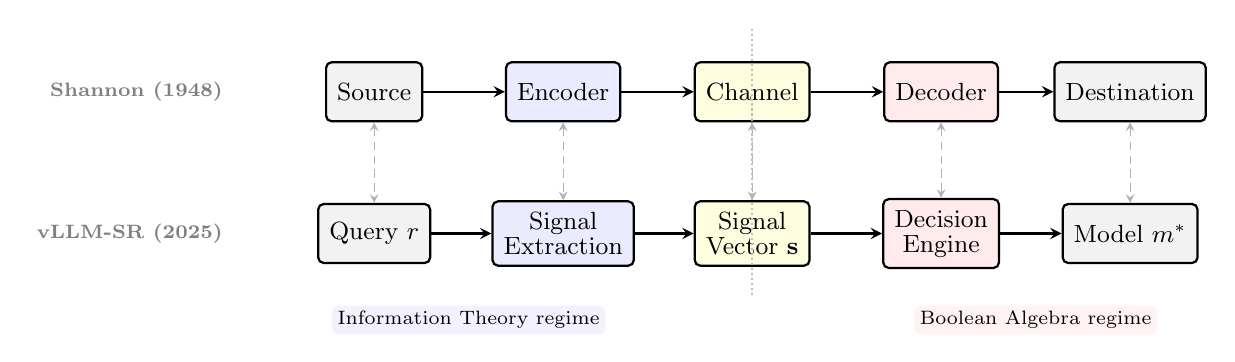
\begin{tikzpicture}[
    sbox/.style={rectangle, draw, thick, rounded corners=2pt,
                 minimum height=0.75cm, align=center, inner sep=4pt, font=\small},
    lbl/.style={font=\scriptsize, text=gray},
    arr/.style={->, >=stealth, thick},
    darr/.style={<->, >=stealth, densely dashed, gray!60, thin},
  ]

  % --- Shannon row (top) ---
  \node[lbl, anchor=east] at (-0.6, 1.8) {\textbf{Shannon (1948)}};
  \node[sbox, fill=black!5]  (src)  at (1.2, 1.8) {Source};
  \node[sbox, fill=blue!8]   (senc) at (3.6, 1.8) {Encoder};
  \node[sbox, fill=yellow!12] (ch)  at (6.0, 1.8) {Channel};
  \node[sbox, fill=red!8]    (sdec) at (8.4, 1.8) {Decoder};
  \node[sbox, fill=black!5]  (dst)  at (10.8, 1.8) {Destination};

  \draw[arr] (src) -- (senc);
  \draw[arr] (senc) -- (ch);
  \draw[arr] (ch) -- (sdec);
  \draw[arr] (sdec) -- (dst);

  % --- VSR row (bottom) ---
  \node[lbl, anchor=east] at (-0.6, 0) {\textbf{vLLM-SR (2025)}};
  \node[sbox, fill=black!5]  (qry) at (1.2, 0) {Query $r$};
  \node[sbox, fill=blue!8]   (sig) at (3.6, 0) {Signal\\[-2pt]Extraction};
  \node[sbox, fill=yellow!12] (sv)  at (6.0, 0) {Signal\\[-2pt]Vector $\mathbf{s}$};
  \node[sbox, fill=red!8]    (dec) at (8.4, 0) {Decision\\[-2pt]Engine};
  \node[sbox, fill=black!5]  (mdl) at (10.8, 0) {Model $m^*$};

  \draw[arr] (qry) -- (sig);
  \draw[arr] (sig) -- (sv);
  \draw[arr] (sv) -- (dec);
  \draw[arr] (dec) -- (mdl);

  % --- Correspondence arrows ---
  \draw[darr] (src.south)  -- (qry.north);
  \draw[darr] (senc.south) -- (sig.north);
  \draw[darr] (ch.south)   -- (sv.north);
  \draw[darr] (sdec.south) -- (dec.north);
  \draw[darr] (dst.south)  -- (mdl.north);

  % --- Regime labels ---
  \draw[densely dotted, gray!50, thick] (6.0, 2.6) -- (6.0, -0.8);
  \node[font=\scriptsize, fill=blue!5, rounded corners=2pt, inner sep=2pt]
    at (2.4, -1.1) {Information Theory regime};
  \node[font=\scriptsize, fill=red!5, rounded corners=2pt, inner sep=2pt]
    at (9.6, -1.1) {Boolean Algebra regime};

  \end{tikzpicture}%
}
  \caption{Structural correspondence between Shannon's communication system~\cite{shannon1948mathematical} and VSR's routing pipeline.
  The dotted line marks the boundary between the information-theoretic regime (signal extraction maximizes mutual information with the routing outcome) and the Boolean-algebraic regime (the decision engine synthesizes routing policies from signal conditions via $\{\wedge, \vee, \neg\}$~\cite{shannon1938symbolic}).}
  \label{fig:shannon_mapping}
\end{figure*}

\begin{figure*}[!ht]
  \centering
  \resizebox{\linewidth}{!}{%
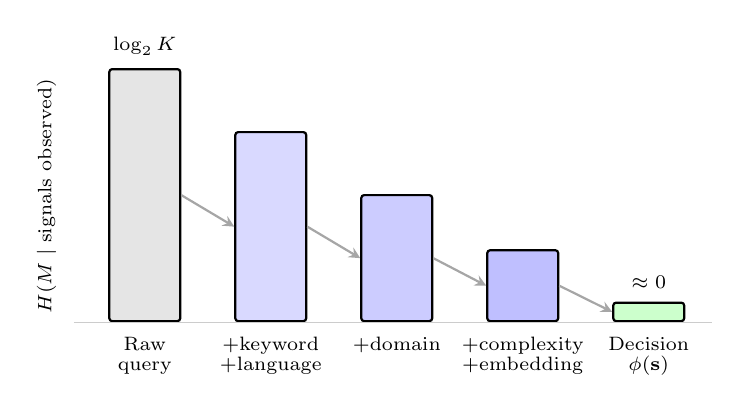
\begin{tikzpicture}[
    bar/.style={draw, thick, rounded corners=1pt, fill=#1, minimum width=0.9cm, anchor=south},
    lbl/.style={font=\scriptsize},
    arr/.style={->, >=stealth, thick, gray!70},
  ]

  % Bars (heights represent entropy)
  \node[bar=gray!20,   minimum height=3.2cm] (b0) at (0.8, 0) {};
  \node[bar=blue!15,   minimum height=2.4cm] (b1) at (2.4, 0) {};
  \node[bar=blue!20,   minimum height=1.6cm] (b2) at (4.0, 0) {};
  \node[bar=blue!25,   minimum height=0.9cm] (b3) at (5.6, 0) {};
  \node[bar=green!20,  minimum height=0.2cm] (b4) at (7.2, 0) {};

  % Bar labels (top)
  \node[lbl, above=1pt of b0] {$\log_2 K$};
  \node[lbl, above=1pt of b1] {};
  \node[lbl, above=1pt of b2] {};
  \node[lbl, above=1pt of b3] {};
  \node[lbl, above=1pt of b4] {$\approx 0$};

  % Bar labels (bottom)
  \node[lbl, below=2pt of b0, align=center] {Raw\\[-1pt]query};
  \node[lbl, below=2pt of b1, align=center] {+keyword\\[-1pt]+language};
  \node[lbl, below=2pt of b2, align=center] {+domain};
  \node[lbl, below=2pt of b3, align=center] {+complexity\\[-1pt]+embedding};
  \node[lbl, below=2pt of b4, align=center] {Decision\\[-1pt]$\phi(\mathbf{s})$};

  % Arrows between bars
  \draw[arr] (b0.east) -- (b1.west);
  \draw[arr] (b1.east) -- (b2.west);
  \draw[arr] (b2.east) -- (b3.west);
  \draw[arr] (b3.east) -- (b4.west);

  % Y-axis label
  \node[font=\scriptsize, rotate=90, anchor=south] at (-0.2, 1.6) {$H(M \mid \text{signals observed})$};

  % Baseline
  \draw[gray!40] (-0.1, 0) -- (8.0, 0);

  \end{tikzpicture}%
}
  \caption{Entropy collapse during signal extraction. Each additional signal reduces the routing uncertainty $H(M \mid \cdot\,)$ from the uniform prior $\log_2 K$ bits until the decision formula $\phi(\mathbf{s})$ yields a near-deterministic model selection.}
  \label{fig:entropy_collapse}
\end{figure*}

This problem is more nuanced than binary difficulty routing.
A production routing system must simultaneously consider:
\begin{itemize}[leftmargin=*]
  \item \textbf{Multi-dimensional signals}: Query domain, modality, complexity, language, user identity, and real-time performance metrics all inform the optimal routing decision.
  \item \textbf{Privacy and safety}: Prompt injection, PII leakage, and hallucinated responses must be detected and mitigated---often with \emph{different policies for different query types and user roles}.
  \item \textbf{Cost-effective model selection}: Algorithms must balance response quality against inference cost and latency, selecting from a heterogeneous pool of local and cloud-hosted models.
  \item \textbf{Deployment diversity}: The same routing framework must serve a privacy-regulated healthcare deployment (strict PII filtering, on-premise models only), a cost-optimized developer tool (aggressive caching, cheapest model first), and a multi-cloud enterprise (failover across providers)---through configuration, not code changes.
  \item \textbf{Multi-turn statefulness}: Routing decisions must be consistent across conversation turns, requiring stateful session management and context preservation.
\end{itemize}

Prior work on LLM routing has made significant progress on individual aspects.
RouteLLM~\cite{ong2024routellm} trains classifiers to route between two models based on query difficulty.
RouterDC~\cite{chen2024routerdc} learns query-model embeddings via dual contrastive learning.
AutoMix~\cite{aggarwal2023automix} formulates cascading as a POMDP.
However, these approaches address model selection in isolation, without integrating signal extraction, safety enforcement, multi-provider backend management, or plugin extensibility into a unified framework.

\subsection{Contributions}

We present \sysname{}, a signal-driven decision routing system whose central innovation is \textbf{composable signal orchestration}: heterogeneous signals are extracted, composed through Boolean rules into deployment-specific decisions, and executed through per-decision plugin chains---enabling a single architecture to serve diverse deployment scenarios.

Our contributions are:

\begin{enumerate}[leftmargin=*]
  \item \textbf{Composable Signal-Decision-Plugin Architecture} (\Cref{sec:architecture,sec:signal_engine,sec:decision_engine,sec:plugins}):
    A three-layer architecture where thirteen signal types are composed through Boolean decision rules into deployment-specific routing policies, with per-decision plugin chains for safety, caching, and augmentation. Different deployment scenarios (privacy-regulated, cost-optimized, multi-cloud) are expressed as different configurations over the same architecture.

  \item \textbf{Semantic Model Routing with Cost-Aware Selection} (\Cref{sec:model_selection}):
    A unified framework integrating thirteen model selection algorithms---rating-based, contrastive, cascading, classical ML, reinforcement learning, and latency-aware---that analyze request semantics to select the most cost-effective model while respecting per-decision privacy and safety constraints.

  \item \textbf{HaluGate: Gated Hallucination Detection} (\Cref{sec:halugate}):
    A three-stage pipeline---sentinel gating, token-level detection, NLI-based explanation---that avoids unnecessary verification on non-factual queries while providing span-level diagnostics when hallucination is detected.

  \item \textbf{Multi-Provider and Multi-Endpoint Routing} (\Cref{sec:extproc}):
    Native support for routing across heterogeneous backends (vLLM, OpenAI, Anthropic, Azure, Bedrock, Gemini, Vertex AI) with provider-specific protocol translation, a pluggable authorization factory for diverse auth mechanisms, weighted multi-endpoint load distribution, and full OpenAI Responses API support for stateful multi-turn conversations.

  \item \textbf{LoRA-Based Multi-Task Classification} (\Cref{sec:lora_mom,sec:ml_inference}):
    A memory-efficient architecture using Low-Rank Adaptation that serves $n$ classification tasks from a single base model with lightweight adapter heads, reducing aggregate model memory from $n$ full copies to one base plus negligible adapter overhead.

  \item \textbf{Episodic Conversation Memory with ReflectionGate} (\Cref{sec:memory_rag}):
    A lightweight memory system that stores raw conversational turns as episodic chunks (filtered by an entropy gate and capped at 16\,KB) rather than relying on LLM-based fact extraction, eliminating inference overhead at write time.
    At retrieval time, a multi-stage \emph{ReflectionGate} pipeline---safety block-pattern filtering, recency decay, Jaccard deduplication, and budget capping---refines retrieved chunks before injection as a separate context message, enabling personalized multi-turn routing without coupling memory quality to an external model.

  \item \textbf{Programmable Neural-Symbolic Configuration Language} (\Cref{sec:dsl}):
    A typed configuration language that serves as the instruction set of the routing inference engine, with a formal grammar parsed into a Boolean expression AST, three-level validation (syntax, reference, constraint), multi-target compilation (flat YAML, Kubernetes CRDs, Helm charts), and round-trip decompilation.
    We formalize the system as a \emph{programmable neural-symbolic inference engine}---neural signal extraction as a hybrid embedding layer, symbolic decision evaluation as Mixture-of-Experts gating---and show that the language's functional completeness enables LLM-based coding agents to synthesize routing policies from natural-language specifications.
\end{enumerate}

\subsection{Paper Organization}

\Cref{sec:architecture} presents the system architecture and composable orchestration model.
\Cref{sec:signal_engine,sec:decision_engine} formalize the signal extraction and decision evaluation layers.
\Cref{sec:plugins,sec:safety,sec:halugate} describe the plugin framework and safety subsystems.
\Cref{sec:lora_mom,sec:ml_inference} detail the LoRA-based classification architecture and multi-runtime inference design.
\Cref{sec:model_selection} surveys the semantic model selection algorithms.
\Cref{sec:extproc} describes the multi-provider request processing pipeline.
\Cref{sec:memory_rag,sec:observability,sec:deployment} cover memory, observability, and deployment.
\Cref{sec:evaluation} presents evaluation results.
\Cref{sec:dsl} specifies the programmable configuration language and develops the neural-symbolic inference engine perspective.
\Cref{sec:related_work} discusses related work, and \Cref{sec:conclusion} concludes.


% --- System Architecture ---
% sections/architecture.tex

\section{System Architecture}
\label{sec:architecture}

We formalize the routing problem and present the three-layer architecture that decomposes it into composable signal extraction, decision evaluation, and plugin execution---enabling a single framework to serve diverse deployment scenarios through configuration.

\subsection{Problem Formulation}

Let $\mathcal{M} = \{m_1, \ldots, m_K\}$ denote a set of $K$ available model backends, each characterized by capability profile, cost, and latency.
Each backend may be served by a different provider $p_k \in \mathcal{P}$ (e.g., local vLLM, OpenAI, Anthropic, Azure, Bedrock, Gemini), with provider-specific API protocols and authentication mechanisms.
A deployment may expose multiple endpoints $\mathcal{E} = \{e_1, \ldots, e_L\}$ with weighted load distribution across backends.

Given an incoming request $r$ (consisting of a message sequence, metadata, user identity, and headers), the routing problem is to:
\begin{enumerate}[leftmargin=*]
  \item Select a model $m^* \in \mathcal{M}$ that maximizes response quality while respecting cost and latency constraints;
  \item Apply deployment-specific safety and privacy transformations $\mathcal{T}(r)$ before and after model invocation;
  \item Route through the correct provider endpoint with appropriate authentication.
\end{enumerate}

Na\"ive approaches either fix $m^*$ statically or route based on a single dimension (e.g., estimated difficulty).
We argue that production routing requires reasoning over \emph{multiple orthogonal signal dimensions simultaneously}, with different \emph{policies} (safety thresholds, caching strategies, prompt augmentation, model pools) for different routing outcomes---and that these policies must be \emph{composable} to support diverse deployment scenarios without architectural changes.

\subsection{Composable Signal Orchestration}

The key architectural innovation is that the same signal extraction, decision evaluation, and plugin execution machinery can be \emph{composed differently} for different deployment scenarios:

\begin{definition}[Deployment Configuration]
A deployment configuration $\Gamma = (\mathcal{S}_\Gamma, \mathcal{D}_\Gamma, \Pi_\Gamma, \mathcal{E}_\Gamma)$ specifies which signal types $\mathcal{S}_\Gamma \subseteq \mathcal{S}$ are active, what decisions $\mathcal{D}_\Gamma$ are evaluated, which plugin chains $\Pi_\Gamma$ are attached, and which endpoints $\mathcal{E}_\Gamma$ are available.
\end{definition}

\noindent\textbf{Example configurations:}
\begin{itemize}[leftmargin=*]
  \item \emph{Privacy-regulated (healthcare)}: Active signals include domain, authz, and language. Decisions route sensitive queries to on-premise models only. Plugins enforce strict PII redaction with no caching.
  \item \emph{Cost-optimized (developer tool)}: Active signals include complexity, embedding, and keyword. Decisions cascade from cheap to expensive models. Plugins enable aggressive semantic caching.
  \item \emph{Multi-cloud enterprise}: Active signals include domain, modality, and authz. Decisions distribute across multiple provider endpoints using latency-aware model selection with weighted failover. Plugins inject provider-specific auth headers.
\end{itemize}

All three scenarios use the same architecture; only $\Gamma$ differs. This composability is the central design contribution.

\subsection{Three-Layer Architecture}

The architecture decomposes routing into three layers, each with a well-defined interface (\Cref{fig:architecture}):

\begin{figure*}[t]
  \centering
  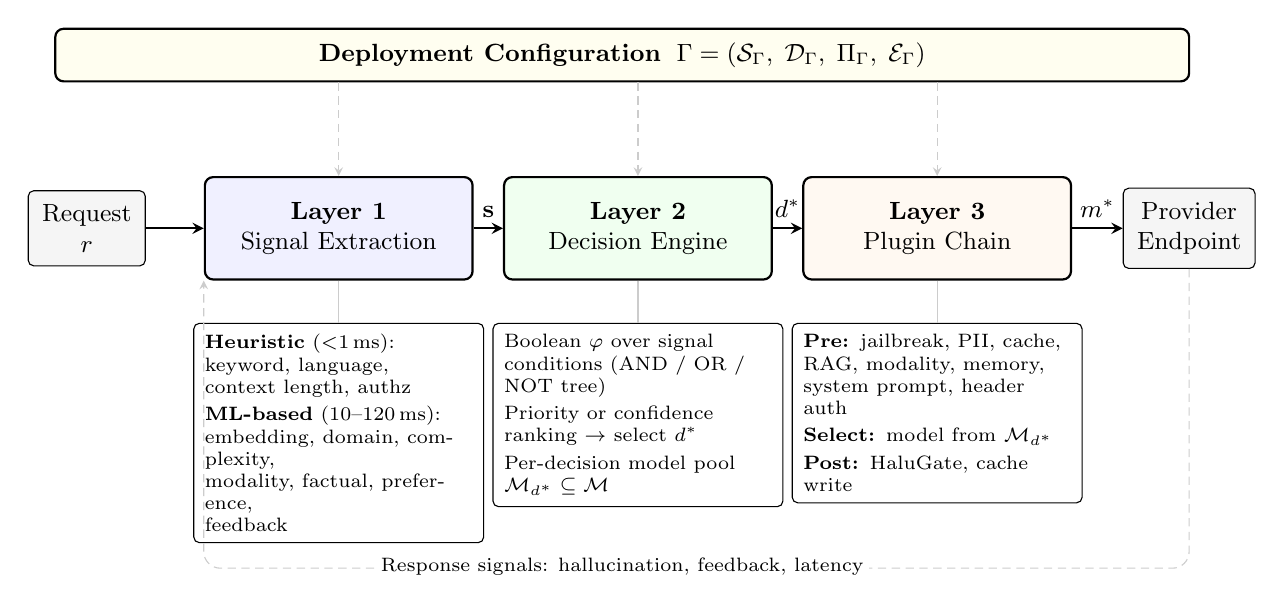
\begin{tikzpicture}[
    layer/.style={rectangle, draw, thick, rounded corners=3pt,
                  minimum height=1.3cm, minimum width=3.4cm, align=center,
                  inner sep=5pt, font=\small},
    io/.style={rectangle, draw, rounded corners=2pt, fill=black!4,
               font=\small, inner sep=5pt, align=center,
               minimum width=1.4cm},
    detail/.style={rectangle, draw, thin, rounded corners=2pt,
                   fill=white, font=\scriptsize, align=left,
                   text width=3.4cm, inner sep=4pt},
    arr/.style={->, >=stealth, thick},
    darr/.style={->, >=stealth, densely dashed, gray!40},
    lbl/.style={font=\small, above, midway},
  ]

  % Configuration bar
  \node[rectangle, draw, thick, rounded corners=3pt, fill=yellow!6,
        minimum width=14.4cm, inner sep=5pt, font=\small]
    (cfg) at (5.6, 3.0)
    {\textbf{Deployment Configuration}\;
     $\Gamma = (\mathcal{S}_\Gamma,\;
     \mathcal{D}_\Gamma,\;
     \Pi_\Gamma,\;
     \mathcal{E}_\Gamma)$};

  % Input
  \node[io] (req) at (-1.2, 0.8) {Request\\$r$};

  % Layer boxes
  \node[layer, fill=blue!6]   (L1) at (2.0,  0.8) {\textbf{Layer 1}\\Signal Extraction};
  \node[layer, fill=green!6]  (L2) at (5.8,  0.8) {\textbf{Layer 2}\\Decision Engine};
  \node[layer, fill=orange!5] (L3) at (9.6, 0.8) {\textbf{Layer 3}\\Plugin Chain};

  % Output
  \node[io] (out) at (12.8, 0.8) {Provider\\Endpoint};

  % Main flow arrows
  \draw[arr] (req)  -- (L1);
  \draw[arr] (L1)   -- node[lbl] {$\mathbf{s}$} (L2);
  \draw[arr] (L2)   -- node[lbl] {$d^*$} (L3);
  \draw[arr] (L3)   -- node[lbl] {$m^*$} (out);

  % Config arrows down
  \draw[darr] (cfg.south -| L1) -- (L1.north);
  \draw[darr] (cfg.south -| L2) -- (L2.north);
  \draw[darr] (cfg.south -| L3) -- (L3.north);

  % Detail boxes
  \node[detail, anchor=north] (d1) at (2.0, -0.4) {%
    \textbf{Heuristic} ({$<$}1\,ms):\\
    keyword, language,\\
    context length, authz\\[2pt]
    \textbf{ML-based} (10--120\,ms):\\
    embedding, domain, complexity,\\
    modality, factual, preference,\\
    feedback};

  \node[detail, anchor=north] (d2) at (5.8, -0.4) {%
    Boolean $\varphi$ over signal\\
    conditions (AND / OR / NOT tree)\\[2pt]
    Priority or confidence\\
    ranking $\to$ select $d^*$\\[2pt]
    Per-decision model pool\\
    $\mathcal{M}_{d^*} \subseteq \mathcal{M}$};

  \node[detail, anchor=north] (d3) at (9.6, -0.4) {%
    \textbf{Pre:} jailbreak, PII, cache,\\
    RAG, modality, memory,\\
    system prompt, header auth\\[2pt]
    \textbf{Select:} model from $\mathcal{M}_{d^*}$\\[2pt]
    \textbf{Post:} HaluGate, cache write};

  % Thin lines connecting layer boxes to detail boxes
  \draw[thin, gray!40] (L1.south) -- (d1.north);
  \draw[thin, gray!40] (L2.south) -- (d2.north);
  \draw[thin, gray!40] (L3.south) -- (d3.north);

  % Feedback loop
  \draw[darr, rounded corners=6pt]
    (out.south) -- ++(0,-3.8) -| (L1.south west);
  \node[font=\scriptsize, fill=white, inner sep=2pt]
    at (5.6, -3.5)
    {Response signals: hallucination, feedback, latency};

  \end{tikzpicture}
  \caption{Three-layer architecture with closed-loop feedback. A deployment configuration~$\Gamma$ selects which signals, decisions, and plugins are active. Layer~1 extracts a signal vector~$\mathbf{s}$ from the request. Layer~2 evaluates Boolean decision formulas to select~$d^*$. Layer~3 executes the per-decision plugin chain, selects a model from~$d^*$'s candidate set, and routes to the provider endpoint. Response-side signals feed back to enable adaptive routing.}
  \label{fig:architecture}
\end{figure*}

\textbf{Layer 1: Signal Extraction.}
The signal layer maps a request $r$ to a structured signal result $\mathbf{s}$, consisting of binary match indicators and real-valued confidences for each configured rule across eleven signal types.
Heuristic signals (keyword, language, context length, authorization) complete in sub-millisecond time.
ML-based signals (embedding similarity, domain classification, factual grounding, modality detection, complexity, preference, user feedback) require neural inference at 10--120\,ms.
Signals are evaluated in parallel, and only signal types referenced by at least one active decision are computed---a critical optimization for deployment configurations that use a subset of available signals.

\textbf{Layer 2: Decision Evaluation.}
The decision layer takes the signal result $\mathbf{s}$ and evaluates a set of decisions $\mathcal{D} = \{d_1, \ldots, d_M\}$, each defined as a Boolean formula over signal conditions.
The engine selects the best-matching decision $d^*$ using either priority-based or confidence-weighted ranking.
Each decision carries its own model candidate set $\mathcal{M}_{d^*} \subseteq \mathcal{M}$, enabling deployment-specific model pools (e.g., a privacy decision restricts candidates to on-premise models).

\textbf{Layer 3: Plugin Chain.}
Each decision $d^*$ carries a per-decision plugin configuration that defines:
(a)~\emph{pre-routing plugins} (jailbreak detection, PII filtering, semantic caching, RAG context injection, modality routing, memory retrieval, system prompt augmentation, header mutation for provider auth), executed before model invocation;
(b)~a \emph{semantic model selection algorithm} applied to $d^*$'s candidate model set $\mathcal{M}_{d^*}$ to find the best model cost-effectively;
(c)~\emph{post-routing plugins} (hallucination detection, cache updates), executed on the model response.

\subsection{Design Principles}

Four principles guide the architecture:

\textbf{Composability.}
Complex routing policies are expressed as compositions of simple primitives: Boolean combinations of signal conditions form decisions; sequences of typed plugins form execution chains; deployment scenarios are expressed as configuration profiles.
This avoids monolithic routing logic and enables the same system to serve fundamentally different deployment requirements.

\textbf{Orthogonality.}
Signals, decisions, and plugins are independent modules with a uniform interface boundary.
New signal types can be added by implementing a single evaluation function---the decision engine references signals solely by type and rule name, requiring no modification.
Likewise, new plugins and providers are registered independently.
The current eleven signal types are the built-in set; the framework is designed to be extended with domain-specific signals as deployment requirements evolve.

\textbf{Closed-loop adaptivity.}
The bidirectional signal flow described in \Cref{sec:signal_engine} enables the architecture to operate as a \emph{closed-loop control system}~\cite{astrom2008feedback}.
In control-theoretic terms, the signal--decision--plugin pipeline is the \emph{plant}, response-side signals (hallucination detection, user feedback, latency measurements) are the \emph{sensors}, and a policy adjustment mechanism is the \emph{controller} that updates decision parameters $\theta^{(t)}$ (priorities, model weights) based on observed response quality:
\begin{equation}
  \theta^{(t+1)} = \theta^{(t)} + \eta \,\nabla_\theta\, \mathbb{E}\bigl[Q\bigl(r,\, m^*(r;\theta^{(t)})\bigr)\bigr]
\end{equation}
where $Q(r, m^*)$ is a response quality metric and $\eta$ is a learning rate.
This formulation connects to the \emph{contextual bandit} framework~\cite{li2010contextual}: the signal vector $S(r)$ serves as the context, model selection is the action, and response quality is the reward.
Standard regret bounds from online learning theory~\cite{shalev2012online} guarantee that the cumulative routing quality of such an adaptive policy converges to that of the best fixed policy in hindsight at a rate of $O(\sqrt{T})$, providing formal performance guarantees for self-improving routing.

\textbf{Per-decision scoping.}
Safety thresholds, caching policies, model candidates, and auth mechanisms are scoped to individual decisions rather than applied globally.
A coding-focused decision can disable PII detection while a customer-support decision enforces strict filtering---using the same system configuration.

\textbf{Provider abstraction.}
The architecture abstracts over provider-specific protocols, authentication, and endpoint topologies.
Multi-endpoint routing with weighted distribution and failover is handled at the infrastructure layer, enabling decisions to reference models by capability rather than by provider-specific endpoint.


% --- Signal Extraction Engine ---
% sections/signal_engine.tex

\section{Signal Extraction Layer}
\label{sec:signal_engine}

The signal extraction layer maps an incoming request $r$ to a structured signal result that characterizes the request along eleven orthogonal dimensions.
We formalize the signal model and describe the extraction algorithms.

\subsection{Signal Model}

\begin{definition}[Signal Rule]
A \emph{signal rule} $\rho = (\tau, n, f)$ consists of a signal type $\tau \in \mathcal{T}$, a rule name $n$, and an evaluation function $f: \mathcal{R} \to \{0, 1\} \times [0, 1]$ that maps a request to a binary match indicator and a confidence score.
\end{definition}

\begin{definition}[Signal Result]
Given a rule set $\mathcal{R} = \{\rho_1, \ldots, \rho_N\}$, the signal result for request $r$ is:
\begin{equation}
  S(r) = \bigl\{ \bigl(\rho_i, \; \mathbf{1}[f_i(r)], \; c_i(r)\bigr) \mid \rho_i \in \mathcal{R} \bigr\}
\end{equation}
where $\mathbf{1}[f_i(r)]$ is the match indicator and $c_i(r) \in [0,1]$ is the confidence.
\end{definition}

The eleven signal types partition into \emph{heuristic} and \emph{learned} categories based on whether they require neural inference.

\subsection{Heuristic Signals}

Heuristic signals use deterministic or statistical algorithms with sub-millisecond latency:

\textbf{Keyword} ($\tau_\text{kw}$).
Rules are defined as pattern sets with Boolean combinators.
Each rule specifies a set of patterns $P = \{p_1, \ldots, p_k\}$ with a combinator $\in \{\textsc{and}, \textsc{or}, \textsc{nor}\}$ and a match mode $\in \{\text{exact}, \text{contains}, \text{regex}\}$.
For \textsc{and}: $f(r) = \bigwedge_{i} \text{match}(p_i, r)$; for \textsc{or}: $f(r) = \bigvee_{i} \text{match}(p_i, r)$.
Confidence is 1.0 on match.

\textbf{Context Length} ($\tau_\text{ctx}$).
Rules define token-count intervals $[l, u]$.
Given estimated token count $t(r)$, the rule matches iff $l \leq t(r) \leq u$.
This enables complexity-aware routing (e.g., short queries to fast models, long contexts to extended-context models).

\textbf{Language} ($\tau_\text{lang}$).
Rules bind detected language codes to named signals using statistical n-gram detection over 100+ languages.
Enables language-specific routing (e.g., CJK queries to multilingual-specialized models).

\textbf{Authorization} ($\tau_\text{authz}$).
Role-based access control signals extracted from request headers, supporting a pluggable authentication factory.
The authz signal layer abstracts over multiple identity providers (API key, OAuth2/OIDC, cloud IAM, custom JWT, LDAP) through provider-specific extractors that resolve user identities and group memberships from credentials.
Role bindings then map resolved identities to named signals, enabling per-role routing policies (e.g., premium users routed to higher-quality models, free-tier users restricted to cost-effective models).
This \emph{inbound} authorization (who is the user and what can they access?) is complementary to the \emph{outbound} authorization factory (\Cref{subsec:authz_factory}) that injects provider-specific credentials when forwarding to backends.

\subsection{Learned Signals}

Learned signals require neural inference, typically 10--100\,ms, using the LoRA-based classifiers described in \Cref{sec:lora_mom}:

\textbf{Embedding Similarity} ($\tau_\text{emb}$).
Each rule defines reference texts $\{t_1, \ldots, t_k\}$ and a similarity threshold $\theta$.
The request embedding $\mathbf{e}_r$ is computed via a shared embedding model, and the rule matches iff:
\begin{equation}
  \max_i \cos(\mathbf{e}_r, \mathbf{e}_{t_i}) \geq \theta
\end{equation}
The confidence equals the maximum cosine similarity.
This provides scalable semantic matching without per-rule model training.

\textbf{Domain Classification} ($\tau_\text{dom}$).
A LoRA-adapted classifier trained on MMLU categories maps requests to domain labels (STEM, humanities, code, creative writing, etc.).
The classification confidence serves as the signal confidence.

\textbf{Factual Grounding} ($\tau_\text{fact}$).
A binary classifier (the HaluGate Sentinel, \Cref{sec:halugate}) determines whether the query requires factual verification, distinguishing factual questions from creative or code-generation tasks.

\textbf{User Feedback} ($\tau_\text{fb}$).
A multi-class classifier detects satisfaction, dissatisfaction, clarification requests, and preference for alternatives, enabling feedback-driven routing adjustments.

\textbf{Modality} ($\tau_\text{mod}$).
A three-class classifier (autoregressive, diffusion, both) determines the appropriate model modality for the request, trained on mixed text-generation and image-generation datasets.

\textbf{Complexity} ($\tau_\text{cpx}$) and \textbf{Preference} ($\tau_\text{pref}$).
Additional learned signals for query difficulty estimation and personalized routing based on user interaction history.

\subsection{Parallel Evaluation with Lazy Computation}

A key optimization is \emph{demand-driven evaluation}: the engine computes only signal types referenced by at least one configured decision.
Let $\mathcal{T}_\text{used} = \bigcup_{d \in \mathcal{D}} \{\tau \mid \exists\, \text{condition in } d \text{ of type } \tau\}$.
Signal evaluators for types in $\mathcal{T}_\text{used}$ are launched as concurrent coroutines, with heuristic signals completing before learned signals due to their sub-millisecond latency.

This demand-driven approach avoids the cost of unused signal types.
In typical configurations with 3--5 active signal types out of eleven, this reduces total signal extraction latency by 50--70\% compared to exhaustive evaluation.

\subsection{Extensibility}

The eleven signal types described above represent the current built-in set; the framework is not limited to these.
The signal extraction layer defines a uniform interface---each signal type implements an evaluation function $f: \mathcal{R} \to \{0,1\} \times [0,1]$---and the decision engine references signals solely by type and rule name.
Adding a new signal type requires only implementing this interface and registering the type; no changes to the decision engine, plugin chain, or deployment infrastructure are needed.
This open architecture allows operators to introduce domain-specific signals (e.g., regulatory compliance classifiers, custom toxicity detectors) alongside the built-in types.

\subsection{Bidirectional Signal Flow}

Signals are not limited to the inbound request path.
The system also extracts signals from model \emph{responses}, enabling closed-loop routing policies that adapt based on output characteristics.
The primary example is \halugate{} (\Cref{sec:halugate}): the Sentinel classifier on the request path determines whether a query requires factual verification (the $\tau_\text{fact}$ signal), and if so, the Detector and Explainer stages analyze the model's response for unsupported claims---producing response-side detection results (confidence scores, hallucinated spans, NLI explanations) that are propagated via HTTP headers or body annotations.
This bidirectional flow---request signals gating which response analyses to perform, and response signals feeding back into observability and policy enforcement---enables adaptive quality assurance without imposing uniform overhead on all requests.

\subsection{Information-Theoretic Signal Analysis}

With $N$ signal types evaluated per request, a natural question is whether all signals contribute independently to routing quality or whether some carry redundant information.
Information theory provides the formal framework for this analysis~\cite{shannon1948mathematical}.

For a signal type $\tau_i$ and the routing outcome variable $Y$ (the selected model), the \emph{mutual information} $I(\tau_i; Y)$ quantifies the reduction in uncertainty about the routing decision provided by observing signal $\tau_i$.
The \emph{conditional mutual information} $I(\tau_i; Y \mid \tau_j)$ measures the additional information from $\tau_i$ given that $\tau_j$ is already observed.
When $I(\tau_i; Y \mid \tau_j) \approx 0$, signals $\tau_i$ and $\tau_j$ are redundant with respect to routing---observing both provides no more discriminative power than observing one.

This analysis enables two optimizations.
First, \emph{adaptive signal pruning}: in a given deployment configuration, signals with near-zero mutual information with the routing outcome can be disabled without affecting routing quality, reducing extraction latency beyond the demand-driven approach of \Cref{sec:signal_engine}.
Second, \emph{information-ordered evaluation}: evaluating high-$I(\tau_i; Y)$ signals first and short-circuiting when the decision outcome is already determined---analogous to early termination in decision trees---can reduce average per-request evaluation cost.
The minimum description length (MDL) principle~\cite{rissanen1978modeling} provides a complementary perspective: the optimal signal subset is the one that describes the routing policy with minimum total code length, balancing signal extraction cost against routing precision.

\paragraph{Contributors.}
Xunzhuo, Huamin Chen, Yossi Ovadia, Liav Weiss, yehudit1987, Xunzhuo, Yue Zhu, Noa Limoy, asaadbalum, abdallahsamabd, Srinivas A, Sophie888, Senan Zedan, Ryan Cook, R3hankhan, Qiping Pan, Nengxing Shen, Avishek Goswami, Avinash Changrani.


% --- Decision Engine ---
% sections/decision_engine.tex

\section{Decision Engine}
\label{sec:decision_engine}

The decision engine evaluates a set of routing decisions against the signal result and selects the best match.
In Shannon's 1938 master's thesis~\cite{shannon1938symbolic}, arbitrary switching-circuit behavior was shown to be representable and minimizable through Boolean algebra---any desired input--output relation over binary signals could be systematically synthesized from $\{\wedge, \vee, \neg\}$.
The decision engine applies this same principle to routing: each routing policy is expressed as a Boolean formula over binary signal conditions, and the functionally complete operator set guarantees that \emph{any} routing policy expressible as a function of the extracted signals can be realized---without modifying the signal layer or the execution layer.
We formalize the decision model, present the evaluation algorithm, and analyze the selection strategies.

\subsection{Decision Model}

\begin{definition}[Decision]
A \emph{decision} $d = (n, \phi, \mathcal{M}_d, \Pi_d, p)$ consists of a name $n$, a Boolean formula $\phi$ over signal conditions, a candidate model set $\mathcal{M}_d \subseteq \mathcal{M}$, a plugin configuration $\Pi_d$, and a priority $p \in \mathbb{Z}$.
\end{definition}

\begin{definition}[Rule Node --- Boolean Expression Tree]
A \emph{rule node} $\phi$ is defined recursively as one of two forms (\Cref{fig:rule_node_tree} illustrates example expression trees):
\begin{itemize}[nosep,leftmargin=1.5em]
  \item \textbf{Leaf} (signal reference): $\phi = \textsc{leaf}(\tau, n)$, referencing a signal type $\tau$ and rule name $n$.
  \item \textbf{Composite} (Boolean operator): $\phi = (\textsc{op}, [\phi_1, \ldots, \phi_k])$, where $\textsc{op} \in \{\textsc{and}, \textsc{or}, \textsc{not}\}$ and $\phi_1, \ldots, \phi_k$ are child rule nodes. $\textsc{not}$ is strictly unary ($k = 1$).
\end{itemize}
Evaluation proceeds by structural recursion:
\begin{equation}
  \text{eval}(\phi, S(r)) =
  \begin{cases}
    \mathbf{1}\bigl[\exists\, (\rho, 1, c) \in S(r) : \rho.\tau = \tau \wedge \rho.n = n\bigr]
      & \text{if } \phi = \textsc{leaf}(\tau, n) \\[4pt]
    \bigwedge_{i=1}^{k} \text{eval}(\phi_i, S(r))
      & \text{if } \textsc{op} = \textsc{and} \\[4pt]
    \bigvee_{i=1}^{k} \text{eval}(\phi_i, S(r))
      & \text{if } \textsc{op} = \textsc{or} \\[4pt]
    \neg\, \text{eval}(\phi_1, S(r))
      & \text{if } \textsc{op} = \textsc{not}
  \end{cases}
\end{equation}
\end{definition}

The recursive structure enables arbitrarily nested Boolean expressions.
Classical flat formulas---a single AND or OR over leaf conditions---are the depth-1 special case and remain the recommended form for simple routing policies.
When richer logic is needed, nesting expresses compound operators directly within a single decision:
$\textsc{nor}(A,B) = \textsc{not}(\textsc{or}(A,B))$;
$\textsc{nand}(A,B) = \textsc{not}(\textsc{and}(A,B))$;
$\textsc{xor}(A,B) = \textsc{or}(\textsc{and}(A, \textsc{not}(B)),\; \textsc{and}(\textsc{not}(A), B))$.
YAML's natural indentation mirrors the logical nesting, preserving readability and auditability even for complex formulas.
Priority-ordered decisions compose multiple such formulas into an ordered evaluation, providing conflict resolution and organizational structure for deployment-scale routing policies.

\begin{figure}[ht]
  \centering
  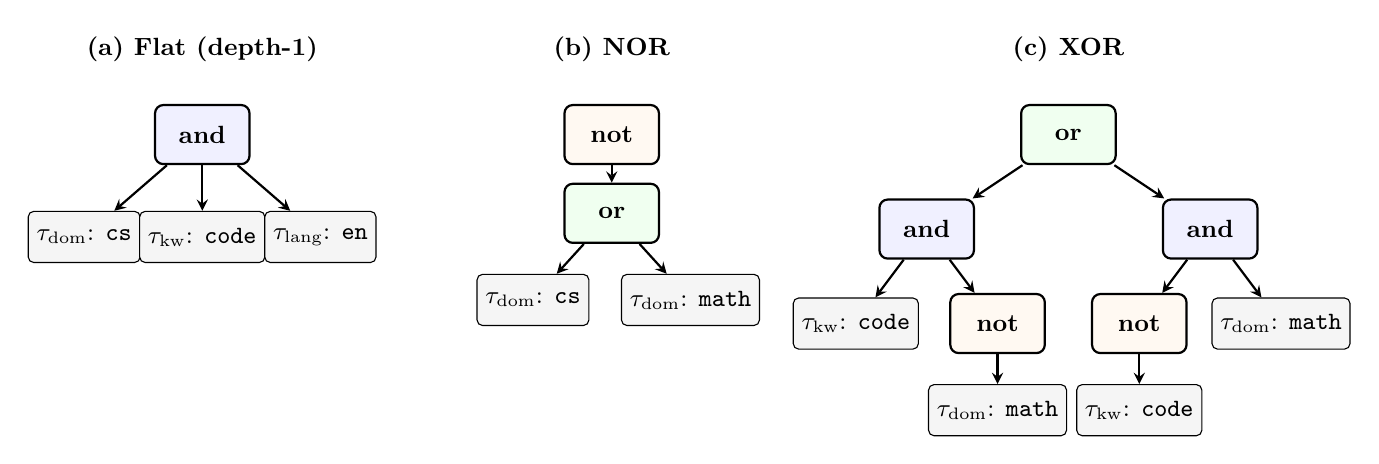
\begin{tikzpicture}[
    gate/.style={rectangle, draw, thick, rounded corners=3pt,
                 minimum height=0.75cm, minimum width=1.2cm,
                 align=center, inner sep=3pt, font=\small\bfseries},
    leaf/.style={rectangle, draw, rounded corners=2pt, fill=black!4,
                 minimum height=0.65cm, align=center,
                 inner sep=3pt, font=\small},
    arr/.style={->, >=stealth, thick},
    lbl/.style={font=\scriptsize, text=gray!70},
  ]

  % --- (a) Flat depth-1: AND(A, B, C) ---
  \node[font=\small\bfseries, anchor=south] at (0, 2.6) {(a) Flat (depth-1)};
  \node[gate, fill=blue!6] (and1) at (0, 1.8) {\textsc{and}};
  \node[leaf] (a1) at (-1.5, 0.5) {$\tau_\text{dom}$: \texttt{cs}};
  \node[leaf] (b1) at (0, 0.5) {$\tau_\text{kw}$: \texttt{code}};
  \node[leaf] (c1) at (1.5, 0.5) {$\tau_\text{lang}$: \texttt{en}};
  \draw[arr] (and1) -- (a1);
  \draw[arr] (and1) -- (b1);
  \draw[arr] (and1) -- (c1);

  % --- (b) NOR: NOT(OR(A, B)) ---
  \node[font=\small\bfseries, anchor=south] at (5.2, 2.6) {(b) NOR};
  \node[gate, fill=orange!5] (not2) at (5.2, 1.8) {\textsc{not}};
  \node[gate, fill=green!6] (or2) at (5.2, 0.8) {\textsc{or}};
  \node[leaf] (a2) at (4.2, -0.3) {$\tau_\text{dom}$: \texttt{cs}};
  \node[leaf] (b2) at (6.2, -0.3) {$\tau_\text{dom}$: \texttt{math}};
  \draw[arr] (not2) -- (or2);
  \draw[arr] (or2) -- (a2);
  \draw[arr] (or2) -- (b2);

  % --- (c) XOR: OR(AND(A, NOT(B)), AND(NOT(A), B)) ---
  \node[font=\small\bfseries, anchor=south] at (11.0, 2.6) {(c) XOR};
  \node[gate, fill=green!6] (or3) at (11.0, 1.8) {\textsc{or}};
  \node[gate, fill=blue!6] (and3l) at (9.2, 0.6) {\textsc{and}};
  \node[gate, fill=blue!6] (and3r) at (12.8, 0.6) {\textsc{and}};
  \draw[arr] (or3) -- (and3l);
  \draw[arr] (or3) -- (and3r);

  % Left branch: AND(A, NOT(B))
  \node[leaf] (a3) at (8.3, -0.6) {$\tau_\text{kw}$: \texttt{code}};
  \node[gate, fill=orange!5] (not3l) at (10.1, -0.6) {\textsc{not}};
  \node[leaf] (b3l) at (10.1, -1.7) {$\tau_\text{dom}$: \texttt{math}};
  \draw[arr] (and3l) -- (a3);
  \draw[arr] (and3l) -- (not3l);
  \draw[arr] (not3l) -- (b3l);

  % Right branch: AND(NOT(A), B)
  \node[gate, fill=orange!5] (not3r) at (11.9, -0.6) {\textsc{not}};
  \node[leaf] (a3r) at (11.9, -1.7) {$\tau_\text{kw}$: \texttt{code}};
  \node[leaf] (b3r) at (13.7, -0.6) {$\tau_\text{dom}$: \texttt{math}};
  \draw[arr] (and3r) -- (not3r);
  \draw[arr] (and3r) -- (b3r);
  \draw[arr] (not3r) -- (a3r);

  \end{tikzpicture}
  \caption{Rule-node expression trees at increasing depth. (a)~A flat depth-1 tree: AND over three leaf conditions. (b)~A NOR expression: $\textsc{not}(\textsc{or}(\text{cs},\text{math}))$, matching all non-STEM queries. (c)~An XOR expression composed from AND, OR, and NOT primitives, routing requests that match exactly one of two signals. Leaf nodes (gray) reference signal conditions; composite nodes use AND (\textcolor{blue!50}{blue}), OR (\textcolor{green!50}{green}), and NOT (\textcolor{orange!45}{orange}).}
  \label{fig:rule_node_tree}
\end{figure}

\subsection{Confidence Computation}

When a decision matches, we compute a confidence score as the mean confidence over satisfied conditions:

\begin{equation}
  \text{conf}(d, S(r)) = \frac{1}{|\Gamma_\text{sat}|} \sum_{\gamma_j \in \Gamma_\text{sat}} c_j(r)
  \label{eq:confidence}
\end{equation}

where $\Gamma_\text{sat} = \{\gamma_j \in \Gamma \mid \text{sat}(\gamma_j, S(r)) = 1\}$ and $c_j(r)$ is the signal confidence for condition $\gamma_j$.
For embedding signals, $c_j$ is the cosine similarity; for heuristic and binary ML signals, $c_j = 1.0$.

\subsection{Selection Strategies}

Given the set of matched decisions $\mathcal{D}_\text{match} = \{d \in \mathcal{D} \mid \text{eval}(\phi_d, S(r)) = 1\}$, two strategies select $d^*$:

\noindent\textbf{Priority Strategy.}
\begin{equation}
  d^* = \arg\max_{d \in \mathcal{D}_\text{match}} p_d
\end{equation}
This provides deterministic, administrator-controlled routing.
Ties are broken by insertion order.

\noindent\textbf{Confidence Strategy.}
\begin{equation}
  d^* = \arg\max_{d \in \mathcal{D}_\text{match}} \text{conf}(d, S(r))
\end{equation}
This enables data-driven routing where embedding similarity and classifier confidence drive selection.

The priority strategy is the default for production deployments where predictability is paramount.
The confidence strategy is preferred for experimental settings where the system should adapt to query characteristics.

\subsection{Evaluation Algorithm}

\begin{algorithm}[t]
\caption{Decision Evaluation}
\label{alg:decision_eval}
\begin{algorithmic}[1]
\REQUIRE Signal result $S(r)$, decisions $\mathcal{D}$, strategy $\sigma \in \{\text{priority}, \text{confidence}\}$
\ENSURE Selected decision $d^*$, confidence $c^*$
\STATE $\mathcal{D}_\text{match} \leftarrow \emptyset$
\FOR{$d \in \mathcal{D}$}
  \IF{$\text{eval}(\phi_d, S(r))$}
    \STATE $c_d \leftarrow \text{conf}(d, S(r))$
    \STATE $\mathcal{D}_\text{match} \leftarrow \mathcal{D}_\text{match} \cup \{(d, c_d)\}$
  \ENDIF
\ENDFOR
\IF{$\sigma = \text{priority}$}
  \STATE $(d^*, c^*) \leftarrow \arg\max_{(d, c) \in \mathcal{D}_\text{match}} p_d$
\ELSE
  \STATE $(d^*, c^*) \leftarrow \arg\max_{(d, c) \in \mathcal{D}_\text{match}} c$
\ENDIF
\RETURN $(d^*, c^*)$
\end{algorithmic}
\end{algorithm}

The algorithm runs in $O(M \cdot L_{\max})$ where $M = |\mathcal{D}|$ is the number of decisions and $L_{\max}$ is the maximum number of conditions per decision.
In practice, $M \leq 50$ and $L_{\max} \leq 10$, making decision evaluation negligible ($< 0.1$\,ms) relative to signal extraction.

\subsection{Expressiveness Analysis}

The recursive rule-node model can express common routing patterns with depth-1 trees (flat formulas) and richer patterns through nesting:

\begin{itemize}[leftmargin=*]
  \item \textbf{Domain routing}: A single leaf condition routes by classified domain.
  \item \textbf{Guarded routing}: AND of a domain condition and a complexity condition routes complex queries within a domain to a capable model.
  \item \textbf{Exclusion routing}: $\textsc{and}(\text{domain}, \textsc{not}(\text{complexity}))$ routes simple queries within a domain to a lightweight model, avoiding the cost of a full-capability model for straightforward requests.
  \item \textbf{Multi-signal routing}: AND of keyword, embedding, and language conditions provides precise routing for specific query patterns.
  \item \textbf{Fallback chains}: Multiple decisions with decreasing priority and progressively broader conditions implement fallback routing.
  \item \textbf{NOR routing} (blanket exclusion): $\textsc{not}(\textsc{or}(\text{cs}, \text{math}, \text{physics}))$ routes all non-STEM queries to a general-purpose model without enumerating every non-STEM domain.
  \item \textbf{NAND routing} (conditional exemption): $\textsc{not}(\textsc{and}(\text{zh}, \text{code}))$ matches all requests \emph{except} Chinese-language code queries, useful for compliance-based routing.
  \item \textbf{XOR routing} (mutual exclusion): $\textsc{or}(\textsc{and}(A, \textsc{not}(B)),\; \textsc{and}(\textsc{not}(A), B))$ routes requests matching exactly one of two signals, enabling exclusive specialization.
  \item \textbf{Nested multi-signal}: $\textsc{and}(\textsc{or}(\text{cs}, \text{math\_kw}),\; \text{en},\; \textsc{not}(\text{long\_ctx}))$ combines disjunctive, conjunctive, and negated sub-trees in a single decision for fine-grained routing.
\end{itemize}

\noindent\textbf{Functional completeness.}
The expressiveness of the recursive rule-node model rests on a classical result from Boolean algebra~\cite{huntington1904sets}: the operator set $\{\wedge, \vee, \neg\}$ is \emph{functionally complete}---any Boolean function $f: \{0,1\}^N \to \{0,1\}$ can be expressed as a formula over these operators.
Because each rule node may nest AND, OR, and NOT to arbitrary depth, a \emph{single} decision formula $\phi$ can already represent any Boolean function over the $N$ signal match indicators---no multi-decision composition is required for completeness.

\begin{proposition}[Single-decision completeness]
For any Boolean function $f: \{0,1\}^N \to \{0,1\}$ over signal match indicators, there exists a rule node $\phi$ using AND, OR, and NOT such that $\text{eval}(\phi, S(r)) = f(S(r))$ for all signal results $S(r)$.
\end{proposition}

\begin{proof}[Proof sketch]
Construct $\phi$ directly from the truth table of $f$.
For each minterm (input assignment where $f = 1$), form an AND-node over the corresponding literals (a leaf $\textsc{leaf}(\tau_i, n_i)$ when the $i$-th signal is 1, or $\textsc{not}(\textsc{leaf}(\tau_i, n_i))$ when it is 0).
Collect all such AND-nodes under a single OR-node.
Since $\{\wedge, \vee, \neg\}$ is functionally complete, the resulting tree evaluates to $f$.
\end{proof}

\begin{proposition}[Routing policy completeness]
For any routing policy $\pi: \{0,1\}^N \to \mathcal{M} \cup \{\bot\}$ mapping signal vectors to model selections, there exists a decision set $\mathcal{D}$ with recursive AND/OR/NOT formulas and priority ordering such that $\pi$ is realized by the evaluation algorithm (\Cref{alg:decision_eval}).
\end{proposition}

\begin{proof}[Proof sketch]
For each model $m_k$ in the range of $\pi$, construct a single decision $d_k$ whose rule node encodes the Boolean function $f_k(\mathbf{s}) = \mathbf{1}[\pi(\mathbf{s}) = m_k]$ using the single-decision completeness result above.
Assign priorities to resolve overlaps deterministically.
\end{proof}

This two-level universality guarantee---completeness within a single decision \emph{and} across a decision set---means the decision engine imposes \emph{no inherent limitation} on what routing policies can be configured.
Priority ordering across decisions is no longer required for expressiveness; it serves as an organizational and conflict-resolution mechanism, equivalent to a decision list~\cite{rivest1987learning} over Boolean features.

\noindent\textbf{Structural analogy to combinational logic circuits.}
The recursive rule-node model maps naturally onto the hierarchy of combinational logic circuits studied in digital design~\cite{brayton1984logic}.
The following table summarizes the correspondence at three levels of generality:

\begin{center}
\begin{tabular}{llp{4.2cm}}
\toprule
\textbf{Circuit Model} & \textbf{Routing System} & \textbf{Expressiveness} \\
\midrule
PLA (two-level)~\cite{fleisher1975introduction}
  & Flat decision (depth-1 tree)
  & Any two-level Boolean function \\
General combinational circuit
  & Recursive rule-node tree
  & Any Boolean function \\
Circuit array + priority encoder
  & Decision set + priority ordering
  & Any routing policy $\pi: \{0,1\}^N \!\to\! \mathcal{M}$ \\
\bottomrule
\end{tabular}
\end{center}

At the first level, a depth-1 rule node---a single AND or OR over leaf conditions---is structurally isomorphic to a \emph{Programmable Logic Array} (PLA)~\cite{fleisher1975introduction}: signal extractors correspond to input lines, leaf conditions to the AND-plane, and the top-level operator to the OR-plane.
At the second level, a recursive rule-node tree corresponds to a general combinational logic circuit---a directed acyclic graph of AND, OR, and NOT gates---where each decision is a complete circuit computing an arbitrary Boolean function.
At the third level, the priority-ordered decision set acts as an array of such circuits with a priority encoder selecting the output, realizing any routing policy.
\Cref{fig:circuit_analogy} illustrates this three-level correspondence.

\begin{figure*}[ht]
  \centering
  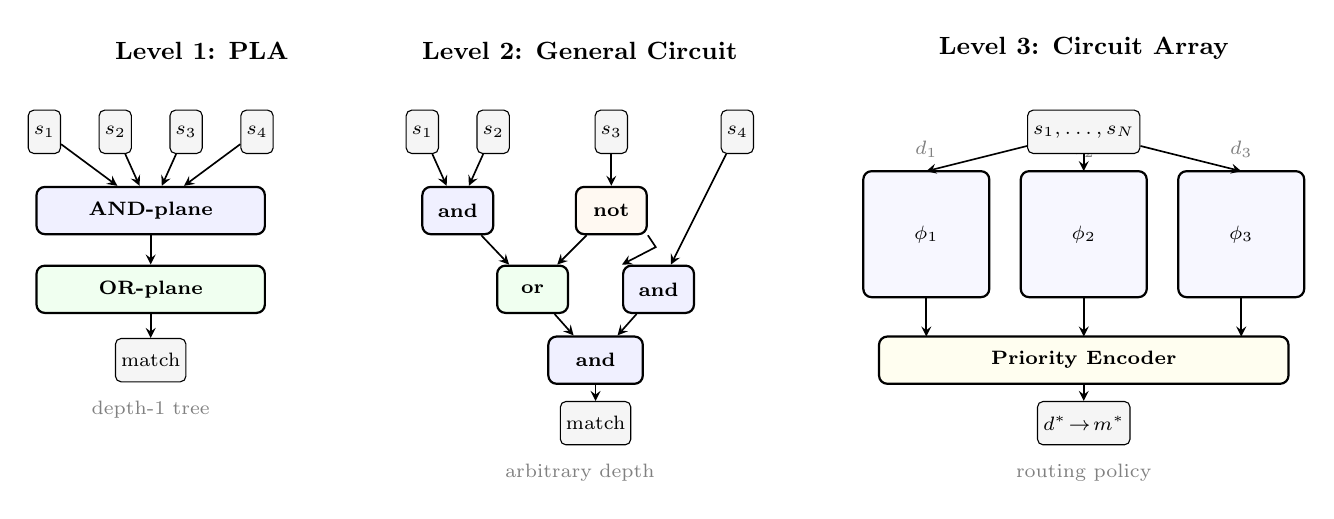
\begin{tikzpicture}[
    gate/.style={rectangle, draw, thick, rounded corners=3pt,
                 minimum height=0.6cm, minimum width=0.9cm,
                 align=center, inner sep=2pt, font=\scriptsize\bfseries},
    io/.style={rectangle, draw, rounded corners=2pt, fill=black!4,
               minimum height=0.55cm, align=center,
               inner sep=2pt, font=\scriptsize},
    prio/.style={rectangle, draw, thick, rounded corners=3pt, fill=yellow!6,
                 minimum height=0.6cm, align=center,
                 inner sep=3pt, font=\scriptsize\bfseries},
    arr/.style={->, >=stealth, semithick},
    darr/.style={->, >=stealth, densely dashed, gray!50},
    brace/.style={decorate, decoration={brace, amplitude=5pt, mirror}},
    titl/.style={font=\small\bfseries, anchor=south},
  ]

  % ===== Level 1: PLA (flat) =====
  \node[titl] at (1.8, 3.6) {Level 1: PLA};

  % Input signals
  \node[io] (s1a) at (-0.2, 2.8) {$s_1$};
  \node[io] (s2a) at (0.7, 2.8) {$s_2$};
  \node[io] (s3a) at (1.6, 2.8) {$s_3$};
  \node[io] (s4a) at (2.5, 2.8) {$s_4$};

  % AND-plane
  \node[gate, fill=blue!6, minimum width=2.9cm] (andp) at (1.15, 1.8) {AND-plane};
  % OR-plane
  \node[gate, fill=green!6, minimum width=2.9cm] (orp) at (1.15, 0.8) {OR-plane};
  % Output
  \node[io] (out1) at (1.15, -0.1) {match};

  \draw[arr] (s1a) -- (andp);
  \draw[arr] (s2a) -- (andp);
  \draw[arr] (s3a) -- (andp);
  \draw[arr] (s4a) -- (andp);
  \draw[arr] (andp) -- (orp);
  \draw[arr] (orp) -- (out1);

  \node[font=\scriptsize, text=gray, anchor=north] at (1.15, -0.5) {depth-1 tree};

  % ===== Level 2: General circuit (recursive) =====
  \node[titl] at (6.6, 3.6) {Level 2: General Circuit};

  % Input signals
  \node[io] (s1b) at (4.6, 2.8) {$s_1$};
  \node[io] (s2b) at (5.5, 2.8) {$s_2$};
  \node[io] (s3b) at (7.0, 2.8) {$s_3$};
  \node[io] (s4b) at (8.6, 2.8) {$s_4$};

  % Gate network
  \node[gate, fill=blue!6] (g1) at (5.05, 1.8) {\textsc{and}};
  \node[gate, fill=orange!5] (g2) at (7.0, 1.8) {\textsc{not}};
  \node[gate, fill=green!6] (g3) at (6.0, 0.8) {\textsc{or}};
  \node[gate, fill=blue!6] (g4) at (7.6, 0.8) {\textsc{and}};
  \node[gate, fill=blue!6, minimum width=1.2cm] (g5) at (6.8, -0.1) {\textsc{and}};

  \draw[arr] (s1b) -- (g1);
  \draw[arr] (s2b) -- (g1);
  \draw[arr] (s3b) -- (g2);
  \draw[arr] (g1) -- (g3);
  \draw[arr] (g2) -- (g3);
  \draw[arr] (g3) -- (g5);
  \draw[arr] (s4b) -- (g4);
  \draw[arr] (g2.south east) -- ++(0.1,-0.15) -- (g4.north west);
  \draw[arr] (g4) -- (g5);

  \node[io] (out2) at (6.8, -0.9) {match};
  \draw[arr] (g5) -- (out2);

  \node[font=\scriptsize, text=gray, anchor=north] at (6.6, -1.3) {arbitrary depth};

  % ===== Level 3: Circuit array + priority encoder =====
  \node[titl] at (13.0, 3.6) {Level 3: Circuit Array};

  % Decision circuits as boxes
  \node[gate, fill=blue!3, minimum width=1.6cm, minimum height=1.6cm,
        draw, thick, rounded corners=3pt] (d1) at (11.0, 1.5) {};
  \node[font=\scriptsize, anchor=center] at (11.0, 1.5) {$\phi_1$};
  \node[font=\scriptsize, text=gray, anchor=south] at (11.0, 2.35) {$d_1$};

  \node[gate, fill=blue!3, minimum width=1.6cm, minimum height=1.6cm,
        draw, thick, rounded corners=3pt] (d2) at (13.0, 1.5) {};
  \node[font=\scriptsize, anchor=center] at (13.0, 1.5) {$\phi_2$};
  \node[font=\scriptsize, text=gray, anchor=south] at (13.0, 2.35) {$d_2$};

  \node[gate, fill=blue!3, minimum width=1.6cm, minimum height=1.6cm,
        draw, thick, rounded corners=3pt] (d3) at (15.0, 1.5) {};
  \node[font=\scriptsize, anchor=center] at (15.0, 1.5) {$\phi_3$};
  \node[font=\scriptsize, text=gray, anchor=south] at (15.0, 2.35) {$d_3$};

  % Input signals shared
  \node[io] (sinp) at (13.0, 2.8) {$s_1, \ldots, s_N$};
  \draw[arr] (sinp) -- (11.0, 2.3);
  \draw[arr] (sinp) -- (13.0, 2.3);
  \draw[arr] (sinp) -- (15.0, 2.3);

  % Priority encoder
  \node[prio, minimum width=5.2cm] (pe) at (13.0, -0.1) {Priority Encoder};
  \draw[arr] (11.0, 0.7) -- (11.0, 0.2);
  \draw[arr] (13.0, 0.7) -- (13.0, 0.2);
  \draw[arr] (15.0, 0.7) -- (15.0, 0.2);

  % Output
  \node[io] (out3) at (13.0, -0.9) {$d^* \!\to\! m^*$};
  \draw[arr] (pe) -- (out3);

  \node[font=\scriptsize, text=gray, anchor=north] at (13.0, -1.3) {routing policy};

  \end{tikzpicture}
  \caption{Three-level correspondence between combinational logic circuits and the decision engine. \textbf{Level~1}: A PLA with AND-plane and OR-plane corresponds to a flat (depth-1) decision formula. \textbf{Level~2}: A general combinational circuit with arbitrarily nested AND, OR, and NOT gates corresponds to a recursive rule-node tree within a single decision. \textbf{Level~3}: An array of circuits with a priority encoder corresponds to the full decision set with priority-ordered evaluation, realizing any routing policy.}
  \label{fig:circuit_analogy}
\end{figure*}

In a PLA, logic is ``programmed'' by setting fuse connections; in a general circuit, by wiring gates; in our system, by YAML configuration whose indentation directly mirrors the gate-level nesting.
This correspondence provides a well-understood theoretical foundation: decades of results on logic minimization, hazard-free design, and testability~\cite{brayton1984logic} apply directly to reasoning about decision optimization and coverage analysis.

\noindent\textbf{Decision set verification and minimization.}
The combinational-logic correspondence makes formal analysis tools from logic synthesis directly applicable to routing configurations.
\emph{Coverage analysis} checks whether every reachable point in the signal space $\{0,1\}^N$ is matched by at least one decision, identifying dead zones where requests would receive no routing directive.
\emph{Conflict detection} identifies signal combinations where multiple decisions match but route to incompatible model pools, flagging ambiguities that priority ordering must resolve.
\emph{Decision minimization}, analogous to the Espresso heuristic for two-level logic optimization~\cite{brayton1984logic} and multi-level logic restructuring~\cite{brayton1984logic}, can reduce a decision set to a minimal equivalent form by merging decisions with compatible conditions and eliminating subsumed rules.
These standard logic-verification techniques become applicable to routing policy validation without adaptation, a direct consequence of the structural isomorphism.

\subsection{Generalization to Fuzzy Evaluation}

The Boolean decision model admits a natural generalization when signal confidence scores are continuous.
Rather than binarizing each signal's output before Boolean combination, we evaluate rule-node trees over the continuous confidence values directly, using fuzzy logic operators~\cite{zadeh1965fuzzy}.

\begin{definition}[Fuzzy Rule-Node Evaluation]
Given continuous signal confidences $c(r) \in [0,1]$ for each leaf condition, the fuzzy evaluation of a rule node $\phi$ is defined by structural recursion:
\begin{equation}
  \widetilde{\text{eval}}(\phi, S(r)) =
  \begin{cases}
    c_\phi(r)
      & \text{if } \phi = \textsc{leaf}(\tau, n) \\[6pt]
    \displaystyle\min_{i=1}^{k}\, \widetilde{\text{eval}}(\phi_i, S(r))
      & \text{if } \textsc{op} = \textsc{and} \\[6pt]
    \displaystyle\max_{i=1}^{k}\, \widetilde{\text{eval}}(\phi_i, S(r))
      & \text{if } \textsc{op} = \textsc{or} \\[6pt]
    1 - \widetilde{\text{eval}}(\phi_1, S(r))
      & \text{if } \textsc{op} = \textsc{not}
  \end{cases}
\end{equation}
where $c_\phi(r)$ is the confidence score of the signal matching leaf $\phi$.
\end{definition}

The operators $(\min, \max, 1{-}x)$ form the standard fuzzy complement triple and satisfy De~Morgan's laws at every level of the tree, preserving the algebraic properties of the crisp model~\cite{bellman1970decision}.
This fuzzy evaluation is a \emph{strict generalization}: when all confidences are binary ($c \in \{0,1\}$), $\min$ reduces to $\wedge$, $\max$ reduces to $\vee$, and $1{-}x$ reduces to $\neg$, so the evaluation coincides exactly with the crisp Boolean model.

The practical consequence is significant.
The current confidence strategy (\Cref{eq:confidence}) uses mean confidence as a tiebreaker \emph{after} binary matching.
Fuzzy evaluation incorporates confidence \emph{during} formula evaluation: a decision with three conditions matched at confidences $(0.95, 0.88, 0.72)$ yields a fuzzy AND score of $0.72$, while a decision with two conditions at $(0.99, 0.98)$ scores $0.98$---correctly preferring the more confident partial match even when both decisions pass binary evaluation.
The functional completeness result of the previous section extends directly: the fuzzy operator triple $(\min, \max, 1{-}x)$ is functionally complete over the continuous lattice $[0,1]$, so any monotone routing policy over continuous signal scores is realizable.

\subsection{Composable Decision Profiles}

The decision model directly enables \emph{composable signal orchestration}: different deployment scenarios are expressed as different decision sets $\mathcal{D}$ over the same signal infrastructure.
A healthcare deployment defines decisions with authz and domain conditions routing to compliant model pools; a developer-tool deployment defines decisions with complexity and keyword conditions routing to cost-optimized cascades; a multi-cloud deployment defines decisions with domain and modality conditions, using latency-aware model selection across provider endpoints.

Formally, switching deployment scenarios corresponds to loading a different decision profile $\mathcal{D}_\Gamma$, while the signal extraction layer $\mathcal{S}$ and plugin implementations $\Pi$ remain unchanged.
This separation of \emph{policy} (what decisions to evaluate) from \emph{mechanism} (how signals are computed and plugins execute) is the architectural basis for the composability claimed in \Cref{sec:architecture}.


\subsection{Interpretation as Mixture-of-Experts Gating}
\label{sec:disc_moe}

The priority-ordered decision evaluation admits a precise structural analogy to the \emph{Mixture-of-Experts} (MoE) gating mechanism~\cite{shazeer2017moe}.
In a standard MoE layer, a gating network $G(\mathbf{x})$ computes a sparse distribution over $K$ expert sub-networks, and the output is a weighted combination of the selected experts' outputs.
In our system:

\begin{itemize}
  \item The \textbf{signal vector} $\mathbf{s}$ plays the role of the shared representation that the gating network operates on.
  \item Each \textbf{decision block} $d_i$ with its Boolean formula $\phi_i(\mathbf{s})$ acts as an \emph{expert gate}---a binary function that determines whether expert~$i$ (a model pool with associated plugins) is activated.
  \item \textbf{Priority ordering} implements \emph{hard routing with early exit}: the first decision whose gate evaluates to true captures the request, analogous to top-1 expert selection in sparse MoE but with a deterministic, priority-based selection rule rather than a learned softmax.
\end{itemize}

\Cref{fig:moe_analogy} formalizes this correspondence.
Unlike standard MoE, the gates here are symbolic (Boolean formulas over interpretable signals) rather than learned softmax projections, which enables formal verifiability and compositional editability.

\begin{figure}[H]
  \centering
  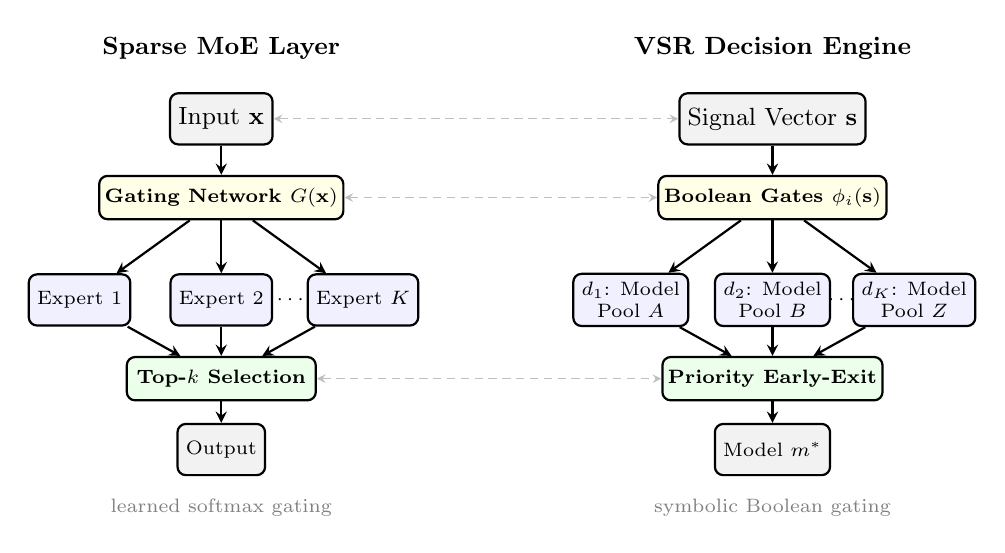
\begin{tikzpicture}[
    box/.style={rectangle, draw, thick, rounded corners=3pt,
                minimum height=0.65cm, align=center, inner sep=3pt, font=\small},
    gate/.style={rectangle, draw, thick, rounded corners=3pt,
                 minimum height=0.55cm, align=center, inner sep=2pt, font=\scriptsize\bfseries},
    arr/.style={->, >=stealth, thick},
    darr/.style={<->, >=stealth, densely dashed, gray!50, thin},
    lbl/.style={font=\scriptsize, text=gray},
  ]

  % === MoE (left) ===
  \node[font=\small\bfseries] at (3.0, 4.0) {Sparse MoE Layer};

  \node[box, fill=black!5] (mx) at (3.0, 3.1) {Input $\mathbf{x}$};
  \node[gate, fill=yellow!10, minimum width=2.4cm] (mg) at (3.0, 2.1) {Gating Network $G(\mathbf{x})$};

  \node[box, fill=blue!6, font=\scriptsize] (me1) at (1.2, 0.8) {Expert 1};
  \node[box, fill=blue!6, font=\scriptsize] (me2) at (3.0, 0.8) {Expert 2};
  \node[box, fill=blue!6, font=\scriptsize] (me3) at (4.8, 0.8) {Expert $K$};
  \node[font=\scriptsize] at (3.9, 0.8) {$\cdots$};

  \node[gate, fill=green!8, minimum width=2.4cm] (msel) at (3.0, -0.2) {Top-$k$ Selection};
  \node[box, fill=black!5, font=\scriptsize] (mout) at (3.0, -1.1) {Output};

  \draw[arr] (mx) -- (mg);
  \draw[arr] (mg) -- (me1);
  \draw[arr] (mg) -- (me2);
  \draw[arr] (mg) -- (me3);
  \draw[arr] (me1) -- (msel);
  \draw[arr] (me2) -- (msel);
  \draw[arr] (me3) -- (msel);
  \draw[arr] (msel) -- (mout);

  \node[lbl, anchor=north] at (3.0, -1.6) {learned softmax gating};

  % === VSR Decision Engine (right) ===
  \node[font=\small\bfseries] at (10.0, 4.0) {VSR Decision Engine};

  \node[box, fill=black!5] (vs) at (10.0, 3.1) {Signal Vector $\mathbf{s}$};
  \node[gate, fill=yellow!10, minimum width=2.4cm] (vg) at (10.0, 2.1) {Boolean Gates $\phi_i(\mathbf{s})$};

  \node[box, fill=blue!6, font=\scriptsize] (vd1) at (8.2, 0.8) {$d_1$: Model\\Pool $A$};
  \node[box, fill=blue!6, font=\scriptsize] (vd2) at (10.0, 0.8) {$d_2$: Model\\Pool $B$};
  \node[box, fill=blue!6, font=\scriptsize] (vd3) at (11.8, 0.8) {$d_K$: Model\\Pool $Z$};
  \node[font=\scriptsize] at (10.9, 0.8) {$\cdots$};

  \node[gate, fill=green!8, minimum width=2.4cm] (vsel) at (10.0, -0.2) {Priority Early-Exit};
  \node[box, fill=black!5, font=\scriptsize] (vout) at (10.0, -1.1) {Model $m^*$};

  \draw[arr] (vs) -- (vg);
  \draw[arr] (vg) -- (vd1);
  \draw[arr] (vg) -- (vd2);
  \draw[arr] (vg) -- (vd3);
  \draw[arr] (vd1) -- (vsel);
  \draw[arr] (vd2) -- (vsel);
  \draw[arr] (vd3) -- (vsel);
  \draw[arr] (vsel) -- (vout);

  \node[lbl, anchor=north] at (10.0, -1.6) {symbolic Boolean gating};

  % Correspondence arrows
  \draw[darr] (mx.east) -- (vs.west);
  \draw[darr] (mg.east) -- (vg.west);
  \draw[darr] (msel.east) -- (vsel.west);

  \end{tikzpicture}
  \caption{Structural analogy between Mixture-of-Experts gating and the VSR decision engine. \textbf{Left}: In a sparse MoE layer, a learned gating network selects top-$k$ experts via softmax. \textbf{Right}: In VSR, Boolean formulas over the signal vector act as symbolic expert gates, with priority ordering implementing deterministic early-exit selection. Dashed arrows mark the structural correspondence.}
  \label{fig:moe_analogy}
\end{figure}

\subsection{Layered Entropy-Folding Interpretation}
\label{sec:disc_entropy_folding}

The priority-ordered gate stack also admits an information-theoretic interpretation as a layered uncertainty-collapse process.
Let $g_\ell(\mathbf{s}) \in \{0,1\}$ denote the match outcome of the $\ell$-th gate under priority order, and let $Z_\ell = g_\ell(\mathbf{s})$.
Define routing uncertainty after $\ell$ evaluated gates as:
\begin{equation}
  U_\ell = H(M \mid \mathbf{s}, Z_{1:\ell})
\end{equation}
where $M$ is the final selected model random variable.
By the chain rule of mutual information:
\begin{equation}
  U_{\ell+1}
  = U_\ell - I\!\left(M;\, Z_{\ell+1}\mid \mathbf{s}, Z_{1:\ell}\right)
  \le U_\ell
\end{equation}
so each additional gate can only maintain or reduce uncertainty.
In this sense, priority depth is \emph{control depth}: a sequence of policy constraints that folds entropy toward a deterministic choice.

\begin{figure}[!ht]
  \centering
  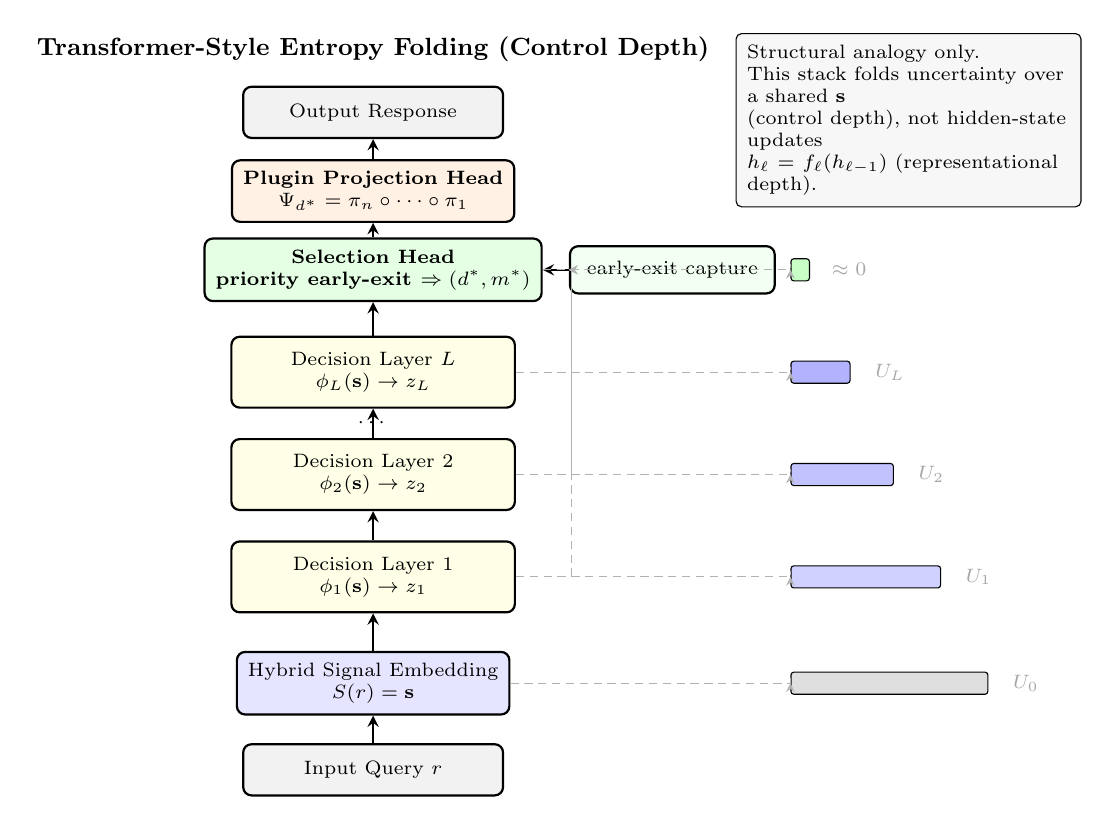
\begin{tikzpicture}[
    box/.style={rectangle, draw, thick, rounded corners=3pt,
                minimum height=0.65cm, minimum width=3.3cm,
                align=center, inner sep=4pt, font=\scriptsize},
    dlayer/.style={rectangle, draw, thick, rounded corners=3pt, fill=yellow!10,
                   minimum height=0.9cm, minimum width=3.6cm,
                   align=center, inner sep=4pt, font=\scriptsize},
    head/.style={rectangle, draw, thick, rounded corners=3pt, fill=green!10,
                 minimum height=0.7cm, minimum width=3.4cm,
                 align=center, inner sep=4pt, font=\scriptsize\bfseries},
    proj/.style={rectangle, draw, thick, rounded corners=3pt, fill=orange!10,
                 minimum height=0.7cm, minimum width=3.4cm,
                 align=center, inner sep=4pt, font=\scriptsize\bfseries},
    arr/.style={->, >=stealth, thick},
    darr/.style={->, >=stealth, densely dashed, gray!60},
    bar/.style={rectangle, draw, rounded corners=1pt, fill=#1, minimum height=0.28cm, anchor=west},
    lbl/.style={font=\scriptsize, text=gray!70},
    note/.style={rectangle, draw, rounded corners=2pt, fill=black!3,
                 text width=4.1cm, align=left, font=\scriptsize, inner sep=4pt}
  ]

  % Title
  \node[font=\small\bfseries] at (3.1, 9.75) {Transformer-Style Entropy Folding (Control Depth)};

  % Main vertical stack
  \node[box, fill=black!5] (inp) at (3.1, 0.6) {Input Query $r$};
  \node[box, fill=blue!10] (emb) at (3.1, 1.7) {Hybrid Signal Embedding\\$S(r)=\mathbf{s}$};

  \node[dlayer] (d1) at (3.1, 3.05) {Decision Layer 1\\$\phi_1(\mathbf{s}) \rightarrow z_1$};
  \node[dlayer] (d2) at (3.1, 4.35) {Decision Layer 2\\$\phi_2(\mathbf{s}) \rightarrow z_2$};
  \node[dlayer] (dL) at (3.1, 5.65) {Decision Layer $L$\\$\phi_L(\mathbf{s}) \rightarrow z_L$};
  \node[font=\scriptsize] at (3.1, 5.0) {$\cdots$};

  \node[head] (sel) at (3.1, 6.95) {Selection Head\\priority early-exit $\Rightarrow (d^*, m^*)$};
  \node[proj] (ph) at (3.1, 7.95) {Plugin Projection Head\\$\Psi_{d^*} = \pi_n \circ \cdots \circ \pi_1$};
  \node[box, fill=black!5] (out) at (3.1, 8.95) {Output Response};

  \draw[arr] (inp) -- (emb);
  \draw[arr] (emb) -- (d1);
  \draw[arr] (d1) -- (d2);
  \draw[arr] (d2) -- (dL);
  \draw[arr] (dL) -- (sel);
  \draw[arr] (sel) -- (ph);
  \draw[arr] (ph) -- (out);

  % Early-exit side path
  \node[box, fill=green!5, minimum width=2.6cm, minimum height=0.6cm] (exit) at (6.9, 6.95) {early-exit capture};
  \draw[darr] (d1.east) -- ++(0.7,0) |- (exit.west);
  \draw[darr] (d2.east) -- ++(0.7,0) |- (exit.west);
  \draw[darr] (dL.east) -- ++(0.7,0) |- (exit.west);
  \draw[arr] (exit.west) -- (sel.east);

  % Entropy folding track
  \node[lbl, font=\scriptsize\bfseries] at (9.6, 7.95) {Entropy Folding};
  \node[bar=gray!25, minimum width=2.5cm] (u0) at (8.4, 1.7) {};
  \node[bar=blue!18, minimum width=1.9cm] (u1) at (8.4, 3.05) {};
  \node[bar=blue!24, minimum width=1.3cm] (u2) at (8.4, 4.35) {};
  \node[bar=blue!30, minimum width=0.75cm] (u3) at (8.4, 5.65) {};
  \node[bar=green!22, minimum width=0.18cm] (uf) at (8.4, 6.95) {};
  \node[lbl, anchor=west] at (11.1, 1.7) {$U_0$};
  \node[lbl, anchor=west] at (10.5, 3.05) {$U_1$};
  \node[lbl, anchor=west] at (9.9, 4.35) {$U_2$};
  \node[lbl, anchor=west] at (9.35, 5.65) {$U_L$};
  \node[lbl, anchor=west] at (8.8, 6.95) {$\approx 0$};
  \draw[darr] (emb.east) -- ++(0.55,0) -| (u0.west);
  \draw[darr] (d1.east) -- ++(0.55,0) -| (u1.west);
  \draw[darr] (d2.east) -- ++(0.55,0) -| (u2.west);
  \draw[darr] (dL.east) -- ++(0.55,0) -| (u3.west);
  \draw[darr] (sel.east) -- ++(0.55,0) -| (uf.west);

  % Boundary note
  \node[note] at (9.9, 8.85)
    {Structural analogy only.\\
     This stack folds uncertainty over a shared $\mathbf{s}$\\
     (control depth), not hidden-state updates\\
     $h_\ell = f_\ell(h_{\ell-1})$ (representational depth).};

  \end{tikzpicture}
  \caption{Transformer-style visualization of layered control depth in VSR.
  Signal extraction constructs a shared embedding $\mathbf{s}$; stacked decision layers apply Boolean gates $\phi_\ell(\mathbf{s})$ that progressively reduce routing uncertainty $U_\ell$; selection resolves $(d^*,m^*)$ via priority early-exit; plugin composition $\Psi_{d^*}$ acts as an output-side projection head over request/response behavior.}
  \label{fig:entropy_folding_layers}
\end{figure}

The MoE analogy also clarifies what the system is \emph{not}: it is not a Transformer in the sequential sense.
Transformer blocks transform the representation layer by layer---each block's output is the next block's input.
In our architecture, all decision blocks operate on the \emph{same} shared signal vector~$\mathbf{s}$; there is no inter-decision information flow.
The priority ordering is an \emph{early-exit mechanism} over parallel evaluations, not a sequential transformation pipeline.
This distinction is important: it means that adding or removing decisions does not affect the behavior of other decisions (modulo priority reordering), a composability property that sequential architectures lack.


% --- Plugin Framework ---
% sections/plugins.tex

\section{Plugin Framework}
\label{sec:plugins}

The plugin layer provides a composable middleware architecture where each matched decision activates an independent chain of typed transformations.
We describe the plugin model and three core infrastructure plugins; safety plugins are covered in \Cref{sec:safety,sec:halugate}, and memory retrieval and RAG injection are covered in \Cref{sec:memory_rag}.

\subsection{Plugin Execution Model}

Formally, a plugin $\pi$ is a typed transformation on the request-response pair:
\begin{equation}
  \pi: (\text{Request}, \text{Context}, \text{Config}_\pi) \to (\text{Request}', \text{Response}') \cup \{\bot\}
\end{equation}
where $\bot$ denotes early termination (e.g., a cache hit returning immediately or a safety violation blocking the request).

Plugins execute in a fixed pipeline order within each decision's chain.
On the \emph{request path}: jailbreak $\to$ PII $\to$ cache $\to$ RAG $\to$ modality $\to$ memory $\to$ system prompt $\to$ header mutation.
On the \emph{response path}: hallucination detection $\to$ cache write.
Each plugin is independently enabled per decision, and its configuration (thresholds, modes, policies) is scoped to that decision.

This per-decision scoping is a key architectural distinction from systems that apply safety and caching globally: it allows differentiated policies for different routing outcomes within the same deployment.

\subsection{Semantic Cache}

The semantic cache exploits the observation that semantically similar queries often produce equivalent responses, avoiding redundant model invocations.

\textbf{Similarity model.}
Given a query $q$ extracted from request $r$, the cache searches for an entry $e$ such that:
\begin{equation}
  \cos(\mathbf{e}_q, \mathbf{e}_e) \geq \theta_d
\end{equation}
where $\mathbf{e}_q, \mathbf{e}_e$ are embeddings computed by the shared embedding model and $\theta_d$ is the per-decision similarity threshold.
On hit, the cached response is returned immediately, bypassing model invocation entirely.

\textbf{Write-through protocol.}
On cache miss, a pending entry is registered before forwarding to the model.
Upon receiving the response, the entry is completed with the response content.
This ensures that concurrent identical queries observe the pending state rather than triggering redundant model calls.

\textbf{Backend abstraction.}
Four backends provide different latency-persistence tradeoffs:
(1)~in-memory HNSW for single-node low-latency deployments;
(2)~Redis for distributed persistent caching;
(3)~Milvus for large-scale approximate nearest neighbor search;
(4)~a hybrid two-tier design combining in-memory HNSW (fast path) with Milvus (persistent store).

\subsection{System Prompt Injection}

Per-decision system prompt injection enables different routing paths to carry different instructions.
Two composition modes are defined:
\begin{itemize}[leftmargin=*]
  \item \textbf{Replace}: Substitutes the entire system message, providing complete control over the model's behavioral context.
  \item \textbf{Insert}: Prepends the decision's prompt to the existing system message, augmenting without overriding user-provided instructions.
\end{itemize}

This enables patterns such as injecting domain-specific instructions for expert routing or safety preambles for sensitive query categories.

\subsection{Header Mutation}

Header mutation enables metadata propagation to downstream model backends via HTTP header modifications (add, update, delete).
This supports use cases including:
backend-specific authentication injection,
routing decision metadata propagation for downstream observability,
and custom signaling to model-serving frameworks (e.g., LoRA adapter selection via headers).

\paragraph{Contributors.}
cryo, Huamin Chen, Xunzhuo, shown, Xunzhuo, Alex Wang, yehudit1987, wangxiaolei, asaadbalum, Yue Zhu, UiJong (Jace) Yang, Srinivas A, Ryan Cook, QIN2DIM, Nengxing Shen, Liav Weiss, Avishek Goswami.


% --- Programmable Neural-Symbolic Configuration Language ---
% sections/dsl_specification.tex

\section{Programmable Neural-Symbolic Configuration Language}
\label{sec:dsl}

While the YAML configuration format described in preceding sections is sufficient for direct human authorship, it conflates two concerns: the \emph{logical specification} of routing policy (signals, decisions, plugins) and the \emph{deployment target} (flat YAML, Kubernetes CRDs, Helm charts).
We introduce a programmable configuration language---the instruction set of the neural-symbolic inference engine (formalized in \Cref{sec:disc_agent})---that separates these concerns, providing a concise, human-readable, and machine-parseable surface syntax for routing policies that compiles to multiple deployment targets through a shared internal representation.

\subsection{Design Goals}

The DSL is designed around four principles:

\begin{enumerate}
  \item \textbf{Conciseness}: Routing policies should read as close to natural language as possible, minimizing syntactic noise relative to YAML.
  \item \textbf{Type safety}: Signal references in Boolean expressions are resolved at compile time; undefined or misspelled signal names produce diagnostics before deployment.
  \item \textbf{Multi-target emission}: A single DSL source compiles to flat YAML (for local development), Kubernetes \texttt{SemanticRouter} CRDs (for operator-based deployment), or Helm \texttt{values.yaml} (for chart-based deployment).
  \item \textbf{Round-trip fidelity}: An existing \texttt{RouterConfig} can be \emph{decompiled} back to DSL source, enabling migration from YAML to DSL and ``round-trip'' editing workflows.
\end{enumerate}

\subsection{Concrete Syntax}
\label{sec:dsl_syntax}

The DSL defines five top-level block types: \texttt{SIGNAL}, \texttt{ROUTE}, \texttt{PLUGIN}, \texttt{BACKEND}, and \texttt{GLOBAL}.
\Cref{fig:dsl_example} shows a representative configuration.

\begin{figure}[!htbp]
\centering
\footnotesize
\begin{verbatim}
SIGNAL domain math { mmlu_categories: ["math"] }
SIGNAL keyword urgent { operator: "any", keywords: ["urgent","asap"] }

PLUGIN safe_pii pii { enabled: true, pii_types_allowed: [] }

ROUTE math_route (description = "Math") {
  PRIORITY 100
  WHEN domain("math")
  MODEL "qwen2.5:3b" (reasoning = true, effort = "high")
  PLUGIN safe_pii
}
ROUTE urgent_ai {
  PRIORITY 200
  WHEN keyword("urgent") AND NOT domain("math")
  MODEL "qwen3:70b" (reasoning = true),
        "qwen2.5:3b" (reasoning = false)
  ALGORITHM confidence { threshold: 0.5 }
}

BACKEND vllm_endpoint ollama { address: "127.0.0.1", port: 11434 }
GLOBAL { default_model: "qwen2.5:3b", strategy: "priority" }
\end{verbatim}
\caption{A representative DSL configuration defining two signals, a reusable plugin template, two routes with Boolean decision logic, a backend endpoint, and global settings.}
\label{fig:dsl_example}
\end{figure}

Each \texttt{SIGNAL} block declares a named signal of a specific type (one of 12 supported types: \texttt{keyword}, \texttt{embedding}, \texttt{domain}, \texttt{fact\_check}, \texttt{user\_feedback}, \texttt{preference}, \texttt{language}, \texttt{context}, \texttt{complexity}, \texttt{modality}, \texttt{authz}, \texttt{jailbreak}, \texttt{pii}).
Each \texttt{ROUTE} block defines a decision with a priority, a Boolean \texttt{WHEN} clause over signal references, one or more model references with optional per-model parameters (reasoning mode, effort level, LoRA adapter, weight), an optional selection algorithm, and zero or more plugin attachments.
\texttt{PLUGIN} blocks at the top level define reusable templates that routes reference by name; inline plugin blocks within routes define route-specific configurations.

\subsection{Grammar and Parsing}
\label{sec:dsl_grammar}

The lexer and parser are implemented using the \texttt{participle} parser-generator library~\cite{participle2024}.
The lexer defines 12 token classes (identifiers, integers, floats, strings, booleans, braces, parentheses, brackets, colon, comma, equals, comments) via regular expressions.
The parser uses a PEG-style grammar with lookahead~3 to resolve ambiguities between signal references and other identifier uses.

The Boolean expression grammar for \texttt{WHEN} clauses follows standard precedence:

\begin{align}
  \textit{BoolExpr} &::= \textit{AndTerm} \;(\texttt{OR}\; \textit{AndTerm})^* \label{eq:bool_or} \\
  \textit{AndTerm} &::= \textit{Factor} \;(\texttt{AND}\; \textit{Factor})^* \label{eq:bool_and} \\
  \textit{Factor} &::= \texttt{NOT}\; \textit{Factor} \mid \texttt{(}\;\textit{BoolExpr}\;\texttt{)} \mid \textit{SignalRef} \label{eq:bool_factor} \\
  \textit{SignalRef} &::= \textit{type}\;\texttt{(}\;\textit{``name''}\;\texttt{)} \label{eq:signal_ref}
\end{align}

This grammar is parsed into a recursive AST (\texttt{BoolAnd}, \texttt{BoolOr}, \texttt{BoolNot}, \texttt{SignalRefExpr} nodes) that the compiler flattens into the \texttt{RuleCombination} tree consumed by the decision engine (\Cref{sec:decision_engine}).
\Cref{fig:bool_ast} illustrates the AST for a representative Boolean expression.

\begin{figure}[!ht]
  \centering
  \resizebox{\linewidth}{!}{%
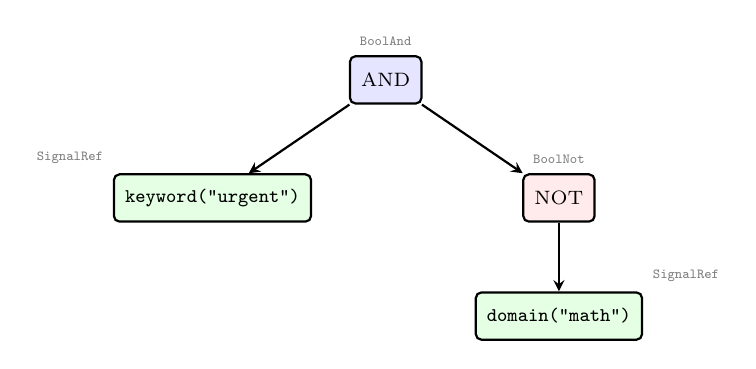
\begin{tikzpicture}[
    tnode/.style={rectangle, draw, thick, rounded corners=2pt,
                  minimum height=0.6cm, align=center, inner sep=4pt, font=\scriptsize},
    arr/.style={->, >=stealth, thick},
    lbl/.style={font=\tiny, text=gray},
  ]

  % Root: AND
  \node[tnode, fill=blue!10] (and) at (0, 0) {AND};
  \node[lbl, anchor=south] at (and.north) {\texttt{BoolAnd}};

  % Left child: keyword("urgent")
  \node[tnode, fill=green!10] (kw) at (-2.2, -1.5) {\texttt{keyword("urgent")}};
  \node[lbl, anchor=south east] at (kw.north west) {\texttt{SignalRef}};

  % Right child: NOT
  \node[tnode, fill=red!8] (not) at (2.2, -1.5) {NOT};
  \node[lbl, anchor=south] at (not.north) {\texttt{BoolNot}};

  % NOT's child: domain("math")
  \node[tnode, fill=green!10] (dom) at (2.2, -3.0) {\texttt{domain("math")}};
  \node[lbl, anchor=south west] at (dom.north east) {\texttt{SignalRef}};

  % Edges
  \draw[arr] (and) -- (kw);
  \draw[arr] (and) -- (not);
  \draw[arr] (not) -- (dom);

  \end{tikzpicture}%
}
  \caption{Boolean expression AST for \texttt{WHEN keyword("urgent") AND NOT domain("math")}. Each leaf is a \texttt{SignalRefExpr} referencing a named signal; internal nodes are Boolean operators (\texttt{BoolAnd}, \texttt{BoolNot}). The compiler flattens this tree into a \texttt{RuleCombination} structure for the decision engine.}
  \label{fig:bool_ast}
\end{figure}

Error recovery is block-granular: if parsing a top-level block fails, the parser splits the input at block boundaries and attempts to parse remaining blocks independently, accumulating partial results alongside error diagnostics.
This enables IDE-like incremental feedback during authoring.

\subsection{Compilation Pipeline}
\label{sec:dsl_compilation}

The compilation pipeline (\Cref{fig:dsl_pipeline}) transforms DSL source through four stages:

\begin{enumerate}
  \item \textbf{Lexing}: The source is tokenized into a stream of typed tokens with position tracking for diagnostic reporting.
  \item \textbf{Parsing}: The token stream is parsed into a \emph{raw parse tree} (participle-generated structs), then lowered to a \emph{resolved AST} (\texttt{Program} $\to$ \texttt{SignalDecl}, \texttt{RouteDecl}, \texttt{PluginDecl}, \texttt{BackendDecl}, \texttt{GlobalDecl}) with desugared values and resolved positions.
  \item \textbf{Compilation}: The AST is compiled to the internal \texttt{RouterConfig} structure. This involves: (a) mapping each \texttt{SIGNAL} block to the appropriate signal configuration (keyword rules, embedding rules, domain categories, etc.); (b) flattening the Boolean expression tree in each \texttt{WHEN} clause into a \texttt{RuleCombination} tree with \texttt{AND}/\texttt{OR}/\texttt{NOT} operators; (c) resolving plugin references against top-level templates with field-level merge semantics (route-local fields override template defaults); and (d) mapping \texttt{BACKEND} blocks to endpoint, provider profile, embedding model, or semantic cache configurations based on the backend type keyword.
  \item \textbf{Emission}: The \texttt{RouterConfig} is serialized to one of three target formats.
\end{enumerate}

\begin{figure*}[!ht]
  \centering
  \resizebox{\linewidth}{!}{%
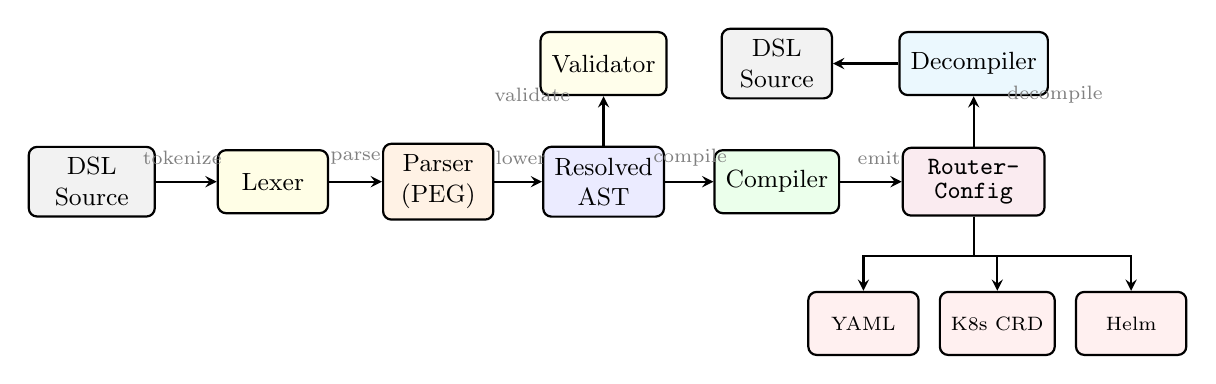
\begin{tikzpicture}[
    box/.style={rectangle, draw, thick, rounded corners=3pt,
                minimum height=0.8cm, align=center, inner sep=4pt, font=\small},
    arr/.style={->, >=stealth, thick},
    lbl/.style={font=\scriptsize, text=gray},
  ]

  % Source
  \node[box, fill=black!5, minimum width=1.6cm] (src) at (0, 0) {DSL\\Source};

  % Lex
  \node[box, fill=yellow!10, minimum width=1.4cm] (lex) at (2.3, 0) {Lexer};

  % Parse
  \node[box, fill=orange!10, minimum width=1.4cm] (parse) at (4.4, 0) {Parser\\(PEG)};

  % AST
  \node[box, fill=blue!8, minimum width=1.4cm] (ast) at (6.5, 0) {Resolved\\AST};

  % Compile
  \node[box, fill=green!8, minimum width=1.5cm] (comp) at (8.7, 0) {Compiler};

  % RouterConfig
  \node[box, fill=purple!8, minimum width=1.8cm] (cfg) at (11.2, 0) {\texttt{Router-}\\[-2pt]\texttt{Config}};

  % Emitters (branching)
  \node[box, fill=red!6, font=\scriptsize, minimum width=1.4cm] (eyaml) at (9.8, -1.8) {YAML};
  \node[box, fill=red!6, font=\scriptsize, minimum width=1.4cm] (ecrd) at (11.5, -1.8) {K8s CRD};
  \node[box, fill=red!6, font=\scriptsize, minimum width=1.4cm] (ehelm) at (13.2, -1.8) {Helm};

  % Decompiler (reverse)
  \node[box, fill=cyan!8, minimum width=1.5cm] (decomp) at (11.2, 1.5) {Decompiler};
  \node[box, fill=black!5, minimum width=1.4cm] (dsout) at (8.7, 1.5) {DSL\\Source};

  % Validator
  \node[box, fill=yellow!8, minimum width=1.4cm] (valid) at (6.5, 1.5) {Validator};

  % Arrows
  \draw[arr] (src) -- (lex);
  \draw[arr] (lex) -- (parse);
  \draw[arr] (parse) -- (ast);
  \draw[arr] (ast) -- (comp);
  \draw[arr] (comp) -- (cfg);

  \draw[arr] (cfg.south) -- ++(0,-0.5) -| (eyaml.north);
  \draw[arr] (cfg.south) -- ++(0,-0.5) -| (ecrd.north);
  \draw[arr] (cfg.south) -- ++(0,-0.5) -| (ehelm.north);

  \draw[arr] (cfg.north) -- (decomp.south);
  \draw[arr] (decomp.west) -- (dsout.east);

  \draw[arr] (ast.north) -- (valid.south);

  % Labels
  \node[lbl] at (1.15, 0.3) {tokenize};
  \node[lbl] at (3.35, 0.3) {parse};
  \node[lbl] at (5.45, 0.3) {lower};
  \node[lbl] at (7.6, 0.3) {compile};
  \node[lbl] at (10.0, 0.3) {emit};
  \node[lbl, anchor=west] at (11.5, 1.1) {decompile};
  \node[lbl, anchor=east] at (6.2, 1.1) {validate};

  \end{tikzpicture}%
}
  \caption{The DSL compilation pipeline. Source text is lexed, parsed into a resolved AST, and compiled to the internal \texttt{RouterConfig}. From this representation, three emitters produce deployment-specific formats (flat YAML, Kubernetes CRD, Helm values). The decompiler reverses the pipeline, reconstructing DSL source from an existing \texttt{RouterConfig}, enabling round-trip editing. The validator operates on the AST directly, producing three-level diagnostics.}
  \label{fig:dsl_pipeline}
\end{figure*}

\subsection{Multi-Target Emission}
\label{sec:dsl_emission}

The shared \texttt{RouterConfig} representation enables three emission targets from a single DSL source:

\begin{itemize}
  \item \textbf{Flat YAML} (\texttt{EmitYAML}): Direct marshaling of \texttt{RouterConfig} for local development and testing. An alternative \texttt{EmitUserYAML} variant restructures the output into the nested \texttt{signals}/\texttt{providers} format expected by the CLI tooling.
  \item \textbf{Kubernetes CRD} (\texttt{EmitCRD}): Wraps the routing logic in a \texttt{SemanticRouter} custom resource (\texttt{vllm.ai/v1alpha1}), mapping backend definitions to \texttt{spec.vllmEndpoints} and routing configuration to \texttt{spec.config}. Signal rules that the CRD schema does not model are preserved as extra fields for ConfigMap-based deployment compatibility.
  \item \textbf{Helm values} (\texttt{EmitHelm}): Nests the \texttt{RouterConfig} under a \texttt{config:} key compatible with the Helm chart's ConfigMap template, pruning zero-value infrastructure sections for clean output.
\end{itemize}

This separation means that infrastructure teams can change deployment targets without modifying the routing policy, and routing engineers can evolve policies without understanding Kubernetes manifests.

\subsection{Decompilation and Round-Trip Editing}
\label{sec:dsl_decompile}

The decompiler reconstructs DSL source text from an existing \texttt{RouterConfig}:

\begin{enumerate}
  \item \textbf{Plugin template extraction}: Plugins used by multiple routes are automatically factored into top-level \texttt{PLUGIN} templates; route-local plugins remain inline.
  \item \textbf{Rule tree reconstruction}: The \texttt{RuleCombination} tree in each decision is walked recursively to reconstruct the Boolean expression with proper \texttt{AND}/\texttt{OR}/\texttt{NOT} operators and parenthesization.
  \item \textbf{Signal type inference}: Signal references in rule nodes are matched against the configuration's signal lists to recover the original signal type keywords.
\end{enumerate}

This enables a migration path: existing YAML configurations can be decompiled to DSL, edited in the more concise syntax, and recompiled to any target format.
The round-trip property ($\text{DSL} \xrightarrow{\text{compile}} \texttt{RouterConfig} \xrightarrow{\text{decompile}} \text{DSL} \xrightarrow{\text{compile}} \texttt{RouterConfig}' \equiv \texttt{RouterConfig}$) is validated by extensive test suites including idempotency and double-round-trip tests.

\subsection{Three-Level Validation}
\label{sec:dsl_validation}

The validator operates on the resolved AST (before compilation) and produces diagnostics at three severity levels:

\begin{enumerate}
  \item \textbf{Error} (Level~1): Syntax errors detected during parsing---malformed blocks, unexpected tokens, missing delimiters. The block-granular error recovery ensures that errors in one block do not prevent analysis of subsequent blocks.
  \item \textbf{Warning} (Level~2): Reference resolution issues---a \texttt{WHEN} clause references a signal name not defined in any \texttt{SIGNAL} block, or a \texttt{PLUGIN} reference has no matching template. The validator performs fuzzy matching on undefined signal names and suggests corrections via \texttt{QuickFix} annotations (e.g., ``did you mean \texttt{math}?'' for a reference to \texttt{mth}).
  \item \textbf{Constraint} (Level~3): Semantic constraint violations---embedding thresholds outside $[0,1]$, port numbers outside valid ranges, negative route priorities, unknown algorithm or signal types. These catch logical errors that are syntactically valid but semantically incorrect.
\end{enumerate}

\Cref{fig:validation_levels} illustrates the three-level diagnostic architecture.
This scheme provides IDE-like progressive feedback, enabling both batch validation (CLI \texttt{validate} command) and interactive authoring with incremental diagnostics.

\begin{figure}[!ht]
  \centering
  \resizebox{\linewidth}{!}{%
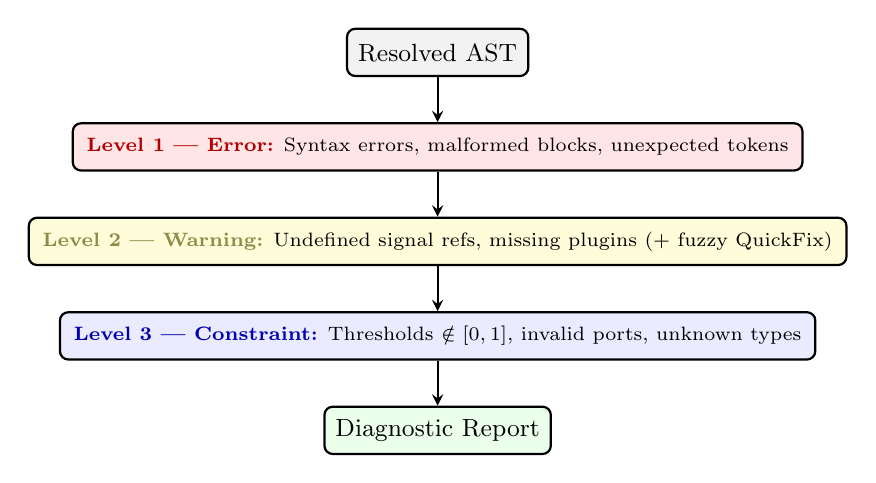
\begin{tikzpicture}[
    box/.style={rectangle, draw, thick, rounded corners=3pt,
                minimum height=0.6cm, minimum width=7.5cm, align=left, inner sep=5pt, font=\scriptsize},
    arr/.style={->, >=stealth, thick},
    lbl/.style={font=\scriptsize\bfseries},
  ]

  % AST input
  \node[rectangle, draw, thick, rounded corners=3pt, fill=black!5,
        minimum height=0.6cm, align=center, inner sep=4pt, font=\small] (ast) at (0, 3.6) {Resolved AST};

  % Level 1
  \node[box, fill=red!10] (l1) at (0, 2.4)
    {\textcolor{red!70!black}{\textbf{Level 1 --- Error:}} Syntax errors, malformed blocks, unexpected tokens};

  % Level 2
  \node[box, fill=yellow!15] (l2) at (0, 1.2)
    {\textcolor{yellow!50!black}{\textbf{Level 2 --- Warning:}} Undefined signal refs, missing plugins (+ fuzzy QuickFix)};

  % Level 3
  \node[box, fill=blue!8] (l3) at (0, 0)
    {\textcolor{blue!70!black}{\textbf{Level 3 --- Constraint:}} Thresholds $\notin [0,1]$, invalid ports, unknown types};

  \draw[arr] (ast) -- (l1);
  \draw[arr] (l1) -- (l2);
  \draw[arr] (l2) -- (l3);

  % Output
  \node[rectangle, draw, thick, rounded corners=3pt, fill=green!8,
        minimum height=0.6cm, align=center, inner sep=4pt, font=\small] (out) at (0, -1.2) {Diagnostic Report};
  \draw[arr] (l3) -- (out);

  \end{tikzpicture}%
}
  \caption{Three-level validation architecture. The validator processes the resolved AST through progressively deeper analysis: syntactic errors (Level~1), reference resolution with fuzzy-matched QuickFix suggestions (Level~2), and semantic constraint checking (Level~3). Diagnostics at all levels are accumulated into a unified report.}
  \label{fig:validation_levels}
\end{figure}

\subsection{DSL as Instruction Set and Agent-Based Policy Synthesis}
\label{sec:disc_agent}

The configuration language can be understood as the \emph{instruction set} of the neural-symbolic inference engine.
Just as a CPU's instruction set defines the space of programs that can execute on the hardware, the DSL defines the space of routing policies that can be instantiated on the signal-decision-plugin architecture.
The functional completeness result of \Cref{sec:decision_engine} guarantees that this instruction set is \emph{universal}: any routing policy $\pi: \{0,1\}^N \to \mathcal{M}$ is expressible.

This framing transforms the problem of \emph{configuring} the router into a \emph{program synthesis} problem (\Cref{fig:agent_synthesis}): given a natural-language specification of routing requirements (``route math queries to the math model, enforce PII filtering for healthcare queries''), synthesize a valid DSL configuration that implements the specification.
This is precisely the class of problems that code-generation agents---LLMs fine-tuned or prompted for program synthesis---are designed to solve.

The DSL's formal grammar and type-safe compilation make it particularly suitable as the target language: the structured syntax---with explicit keywords, typed blocks, and a finite set of signal types---constrains the generation space far more tightly than free-form YAML, reducing the probability of syntactically valid but semantically incorrect configurations.
The three-level validator provides immediate, machine-readable feedback that a coding agent can use to iteratively refine generated configurations.

\begin{figure*}[!ht]
  \centering
  \resizebox{\linewidth}{!}{%
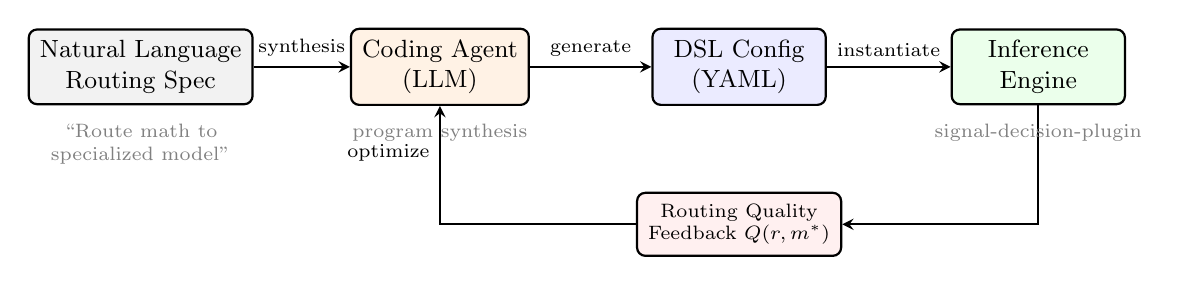
\begin{tikzpicture}[
    box/.style={rectangle, draw, thick, rounded corners=3pt,
                minimum height=0.8cm, align=center, inner sep=4pt, font=\small},
    arr/.style={->, >=stealth, thick},
    lbl/.style={font=\scriptsize, text=gray},
  ]

  % Natural language spec
  \node[box, fill=black!5, minimum width=2.2cm] (nl) at (0, 0) {Natural Language\\Routing Spec};

  % Coding Agent
  \node[box, fill=orange!10, minimum width=2.2cm] (agent) at (3.8, 0) {Coding Agent\\(LLM)};

  % DSL Config
  \node[box, fill=blue!8, minimum width=2.2cm] (dsl) at (7.6, 0) {DSL Config\\(YAML)};

  % Inference Engine
  \node[box, fill=green!8, minimum width=2.2cm] (engine) at (11.4, 0) {Inference\\Engine};

  % Feedback loop
  \node[box, fill=red!6, minimum width=2.0cm, font=\scriptsize] (fb) at (7.6, -2.0) {Routing Quality\\Feedback $Q(r, m^*)$};

  \draw[arr] (nl) -- node[above, font=\scriptsize] {synthesis} (agent);
  \draw[arr] (agent) -- node[above, font=\scriptsize] {generate} (dsl);
  \draw[arr] (dsl) -- node[above, font=\scriptsize] {instantiate} (engine);
  \draw[arr] (engine.south) |- (fb.east);
  \draw[arr] (fb.west) -| node[left, font=\scriptsize, pos=0.8] {optimize} (agent.south);

  % Labels
  \node[lbl, anchor=north] at (0, -0.6) {``Route math to};
  \node[lbl, anchor=north] at (0, -0.9) {specialized model''};
  \node[lbl, anchor=north] at (3.8, -0.6) {program synthesis};
  \node[lbl, anchor=north] at (11.4, -0.6) {signal-decision-plugin};

  \end{tikzpicture}%
}
  \caption{Agent-based policy synthesis pipeline. A coding agent (LLM) translates natural-language routing specifications into DSL configurations, which are instantiated on the inference engine. Routing quality feedback closes the loop, enabling iterative policy refinement. The DSL's functional completeness guarantees that any expressible routing policy is reachable by the synthesis process.}
  \label{fig:agent_synthesis}
\end{figure*}

The connection to reinforcement learning is direct: the coding agent's policy $\pi_\theta(\text{config} \mid \text{spec})$ can be optimized via RLHF or rule-based reward~\cite{zhang2025routerr1}, where the reward signal is the downstream routing quality $Q(r, m^*)$ aggregated over a traffic distribution.
This operates at a \emph{meta-level} compared to prior work on RL-based routing~\cite{zhang2025routerr1}: rather than learning to route individual requests, the agent learns to \emph{write routing policies} that generalize across request distributions.
The DSL provides the structured action space that makes this meta-learning tractable---the agent generates a finite, syntactically constrained configuration rather than an arbitrary neural network.

\subsection{Synthesis: A Programmable Neural-Symbolic Inference Engine}

Taken together, the signal extraction layer (\Cref{sec:signal_engine}), decision engine (\Cref{sec:decision_engine}), and configuration language characterize the system as a \textbf{programmable neural-symbolic inference engine}:

\begin{enumerate}
  \item \textbf{Neural front-end}: The signal extraction layer uses both heuristic and learned (neural) methods to produce a structured representation---analogous to a hybrid embedding layer (\Cref{sec:disc_embedding}).
  \item \textbf{Symbolic back-end}: The decision engine applies Boolean logic over the structured representation---analogous to symbolic expert gating with formal verifiability (\Cref{sec:disc_moe}).
  \item \textbf{Programmable interface}: The DSL configuration is the ``program'' that specifies the inference behavior, and the functional completeness of the Boolean decision model guarantees universality of the program space.
  \item \textbf{Agent-compilable}: The structured DSL enables LLM-based coding agents to serve as ``compilers'' from natural-language specifications to executable routing policies, with RL-based optimization closing the loop.
\end{enumerate}

This perspective unifies the Shannon-theoretic foundation (information reduction + Boolean synthesis) with the modern ML landscape (embeddings + MoE gating + agent-based program synthesis), and suggests that the architecture occupies a principled point in the design space between fully neural routing systems (which sacrifice interpretability and editability) and fully manual rule systems (which sacrifice adaptivity and scalability).



% --- Safety: Jailbreak + PII ---
% sections/safety.tex

\section{Request-Time Safety: Jailbreak and PII Detection}
\label{sec:safety}

Request-time safety plugins detect adversarial inputs and sensitive information before queries reach model backends.
Both operate as gating plugins that can terminate request processing with an immediate rejection.

\subsection{Jailbreak Detection}

Jailbreak attacks~\cite{jain2023promptguard} attempt to override model safety instructions through adversarial prompt construction.
Our detection pipeline addresses this as a binary classification problem with per-decision sensitivity control.

\textbf{Formulation.}
Given a text input $x$ (the user's latest message, or the full conversation history when context-aware detection is enabled), a classifier $g_\text{jb}$ produces:
\begin{equation}
  g_\text{jb}(x) = (y, c) \in \{\textsc{benign}, \textsc{injection}, \textsc{jailbreak}\} \times [0, 1]
\end{equation}
The request is blocked iff $y \neq \textsc{benign}$ and $c \geq \theta_d$, where $\theta_d$ is the per-decision threshold.

\textbf{Classifier architecture.}
We support four inference backends with varying context-length and deployment characteristics:
(1)~BERT with LoRA adapters (standard context);
(2)~ModernBERT~\cite{warner2024modernbert} with Flash Attention;
(3)~mmBERT-32K with YaRN RoPE for 32K-token contexts;
(4)~external vLLM-served guardrail models for decoupled scaling.
All local backends use the LoRA adapter architecture (\Cref{sec:lora_mom}), reducing model memory footprint.

\textbf{Per-decision sensitivity.}
Different decisions configure different thresholds: a public-facing endpoint might use $\theta = 0.7$ for aggressive detection, while an internal developer tool uses $\theta = 0.95$ to minimize false positives.
History inclusion is also per-decision: some decisions analyze only the latest message (low latency), while others analyze the full conversation (higher recall for multi-turn attacks).

\subsection{PII Detection}

PII detection identifies personally identifiable information at the token level and enforces configurable allow/deny policies.

\textbf{Formulation.}
A token classifier $g_\text{pii}$ operates on the input sequence $x = (x_1, \ldots, x_T)$ and produces BIO-tagged predictions:
\begin{equation}
  g_\text{pii}(x) = \bigl\{(i, j, \ell, c) \mid \text{span } x_i \ldots x_j \text{ is PII type } \ell \text{ with confidence } c\bigr\}
\end{equation}
where $\ell \in \{\textsc{person}, \textsc{email}, \textsc{phone}, \textsc{ssn}, \textsc{credit\_card}, \ldots\}$.

\textbf{Policy model.}
Detected PII entities are evaluated against a per-decision policy:
\begin{equation}
  \text{allowed}(\ell) =
  \begin{cases}
    \ell \notin \mathcal{L}_\text{deny} & \text{if allow-by-default} \\
    \ell \in \mathcal{L}_\text{allow} & \text{otherwise}
  \end{cases}
\end{equation}
If any entity $(\cdot, \cdot, \ell, c)$ satisfies $c \geq \theta_d$ and $\neg\text{allowed}(\ell)$, the request is blocked.

This two-mode policy (allow-by-default with deny list, or deny-by-default with allow list) provides flexible control: a medical application might allow \textsc{person} while blocking \textsc{ssn}, whereas a general chatbot might block all PII types.

\subsection{Safety Pipeline Ordering}

Jailbreak detection executes before PII detection, ensuring that adversarial inputs designed to bypass PII detection are caught first.
Both use the LoRA adapter architecture (\Cref{sec:lora_mom}), and when run concurrently via parallel goroutines, the wall-clock time is dominated by the slower of the two classifiers rather than their sum.

\paragraph{Contributors.}
Xunzhuo, Xunzhuo, Huamin Chen, Jintao Zhang, yehudit1987, shown, cryo, Jared, asaadbalum, Noa Limoy, Liav Weiss.


% --- HaluGate ---
% sections/halugate.tex

\section{HaluGate: Gated Hallucination Detection}
\label{sec:halugate}

Hallucination---generating plausible but unsupported content---is a fundamental limitation of autoregressive language models~\cite{manakul2023selfcheckgpt,min2023factscore}.
We introduce \halugate{}, a three-stage pipeline that addresses a key efficiency challenge: most queries (creative writing, code generation, brainstorming) do not require factual verification, yet na\"ive hallucination detection incurs overhead on every response.

\subsection{Design Rationale}

Existing approaches apply hallucination detection uniformly to all responses~\cite{manakul2023selfcheckgpt} or require multiple response samples~\cite{min2023factscore}.
\halugate{} introduces two innovations:
(1)~a \emph{gating stage} that skips verification for non-factual queries, amortizing detection cost over the query distribution; and
(2)~a \emph{span-level} detection and explanation pipeline that identifies \emph{which} tokens are hallucinated and \emph{why}, rather than providing only a binary judgment.

\subsection{Three-Stage Pipeline}

\textbf{Stage 1: Sentinel (Gating).}
A lightweight binary classifier $g_\text{sent}$ determines whether the query warrants factual verification:
\begin{equation}
  g_\text{sent}(q) \in \{\textsc{needs\_fact\_check}, \textsc{no\_fact\_check}\}
\end{equation}
If $g_\text{sent}(q) = \textsc{no\_fact\_check}$, Stages 2--3 are skipped entirely.
The Sentinel operates on the request text and is implemented as a LoRA-adapted classifier sharing the base model with other signal extractors.
In practice, 40--60\% of queries are classified as non-factual, proportionally reducing the average detection cost.

The Sentinel also serves dual duty as the \texttt{fact\_check} signal in the signal extraction layer (\Cref{sec:signal_engine}), enabling decisions to incorporate factual grounding into routing logic.

\textbf{Stage 2: Detector (Span Identification).}
A token-level classifier $g_\text{det}$ identifies hallucinated spans in the model response:
\begin{equation}
  g_\text{det}(q, \mathbf{c}, a) = \bigl\{(i, j, c_{ij}) \mid a_i \ldots a_j \text{ is unsupported by context } \mathbf{c}\bigr\}
\end{equation}
where $q$ is the user query, $\mathbf{c}$ is the grounding context (user-provided context and tool-call results), $a$ is the assistant's response, and $(i, j, c_{ij})$ denotes a flagged span with confidence.

When tool-calling is present, tool execution results provide high-quality ground truth: database query results, API responses, and calculations serve as authoritative context $\mathbf{c}$, substantially improving detection precision.

\textbf{Stage 3: Explainer (NLI Classification).}
For each flagged span $(i, j)$, a Natural Language Inference (NLI) model~\cite{williams2018mnli} classifies the relationship between the span and the grounding context:
\begin{equation}
  g_\text{nli}(a_{i:j}, \mathbf{c}) \in \{\textsc{entailment}, \textsc{contradiction}, \textsc{neutral}\}
\end{equation}
This distinguishes between content that \emph{contradicts} the context (definitive hallucination) and content that is merely \emph{unsupported} (potential hallucination), providing actionable diagnostics.

\subsection{Cost Analysis}

Let $p_\text{factual}$ be the fraction of queries requiring factual verification, $C_\text{sent}$, $C_\text{det}$, $C_\text{nli}$ be the costs of each stage, and $\bar{k}$ be the average number of flagged spans.
The expected cost per query is:
\begin{equation}
  \mathbb{E}[\text{Cost}] = C_\text{sent} + p_\text{factual} \cdot \bigl(C_\text{det} + \bar{k} \cdot C_\text{nli}\bigr)
\end{equation}

Since the Sentinel is a lightweight LoRA-adapted classifier (\Cref{sec:lora_mom}) that runs concurrently with other signal extractors, its wall-clock cost is largely hidden behind other ML signals.
For a workload with $p_\text{factual} = 0.5$, the gating stage reduces the expected Detector and Explainer cost by approximately 50\% compared to applying full detection to all responses.

\subsection{Action Policies}

\halugate{} supports four configurable response actions:

\begin{table}[h]
\centering
\caption{\halugate{} action policies upon hallucination detection}
\label{tab:halugate_actions}
\begin{tabular}{lp{8cm}}
\toprule
\textbf{Action} & \textbf{Semantics} \\
\midrule
\texttt{block}  & Reject the response; return an error to the client. Appropriate for high-stakes factual applications. \\
\texttt{header} & Propagate detection metadata via HTTP headers, enabling downstream policy enforcement by the client or API gateway. \\
\texttt{body}   & Prepend a warning to the response body, alerting users to potential inaccuracies. \\
\texttt{none}   & Log detection results without modifying the response. Useful for monitoring and threshold calibration. \\
\bottomrule
\end{tabular}
\end{table}

The progressive architecture enables incremental deployment: organizations begin with Sentinel-only gating (signal-layer integration at minimal cost), add the Detector for span-level monitoring, and enable the Explainer for full diagnostic output.

\paragraph{Contributors.}
Huamin Chen, Xunzhuo, Yossi Ovadia, yehudit1987, Yue Zhu, Xunzhuo, shown, OneZero-Y, abdallahsamabd.


% --- Modular LoRA + MoM Family ---
% sections/lora_mom.tex

\section{LoRA-Based Multi-Task Classification and MoM Model Family}
\label{sec:lora_mom}

Signal-driven routing requires multiple classification tasks on the critical path of every request.
Na\"ively, each task requires a separate fine-tuned model, creating a memory scaling problem.
We describe the LoRA-based architecture that addresses this and the purpose-built model family trained for semantic routing.

\subsection{Problem: Linear Memory Scaling}

Let $n$ denote the number of active classification tasks (domain, jailbreak, PII, fact-check, feedback, modality).
With independently fine-tuned models, the total model memory is:
\begin{equation}
  M_\text{indep} = n \cdot |\theta_\text{base}|
\end{equation}
where $|\theta_\text{base}|$ is the parameter count of a single base model.
For $n = 6$ tasks with a 150M-parameter base model, this requires storing and loading six full model copies ($\sim$900M parameters total)---a significant memory burden, especially in GPU-constrained environments.

Additionally, managing $n$ independent model checkpoints complicates deployment, versioning, and updates.

\subsection{Solution: Single Base Model with LoRA Adapters}

Low-Rank Adaptation (LoRA)~\cite{hu2022lora} represents task-specific weight modifications as low-rank decompositions:
\begin{equation}
  W'_i = W + \Delta W_i = W + B_i A_i, \quad B_i \in \mathbb{R}^{d \times r}, \; A_i \in \mathbb{R}^{r \times d}
\end{equation}
where $W$ is the shared base weight, $r \ll d$ is the adapter rank, and $B_i A_i$ is the task-specific perturbation.

The aggregate model memory becomes:
\begin{equation}
  M_\text{LoRA} = |\theta_\text{base}| + \sum_{i=1}^{n} 2 r d = |\theta_\text{base}| + n \cdot 2rd
\end{equation}

With rank $r = 32$ and hidden dimension $d = 768$, each adapter adds $2 \times 32 \times 768 = 49{,}152$ parameters ($\sim$0.02\% of the base model).
For $n = 6$, total adapter overhead is $\sim$295K parameters---negligible compared to the 150M-parameter base.

\noindent\textbf{Memory reduction.}
\begin{equation}
  \frac{M_\text{LoRA}}{M_\text{indep}} = \frac{|\theta_\text{base}| + n \cdot 2rd}{n \cdot |\theta_\text{base}|} \approx \frac{1}{n} \quad \text{for } 2nrd \ll |\theta_\text{base}|
\end{equation}
At $n = 6$, this yields $\sim$6$\times$ memory reduction: one 150M-parameter model plus six tiny adapters instead of six full copies.

\subsection{Inference Architecture}

Each classification task proceeds as a full forward pass through the base model with the task-specific LoRA perturbation applied (\Cref{fig:lora_arch}):

\begin{enumerate}
  \item \textbf{Load}: A single base model is loaded into GPU/CPU memory at startup. Each LoRA adapter (a pair of small matrices per adapted layer) is loaded alongside it.
  \item \textbf{Inference}: For each classification task $i$, the base model runs a forward pass with adapter $i$'s weights merged: $W'_i = W + B_i A_i$. Each task still requires its own forward pass.
  \item \textbf{Parallelism}: Multiple classification tasks execute concurrently via parallel threads/goroutines. Wall-clock time is determined by the slowest classifier, not the sum.
\end{enumerate}

\begin{figure}[ht]
    \centering
    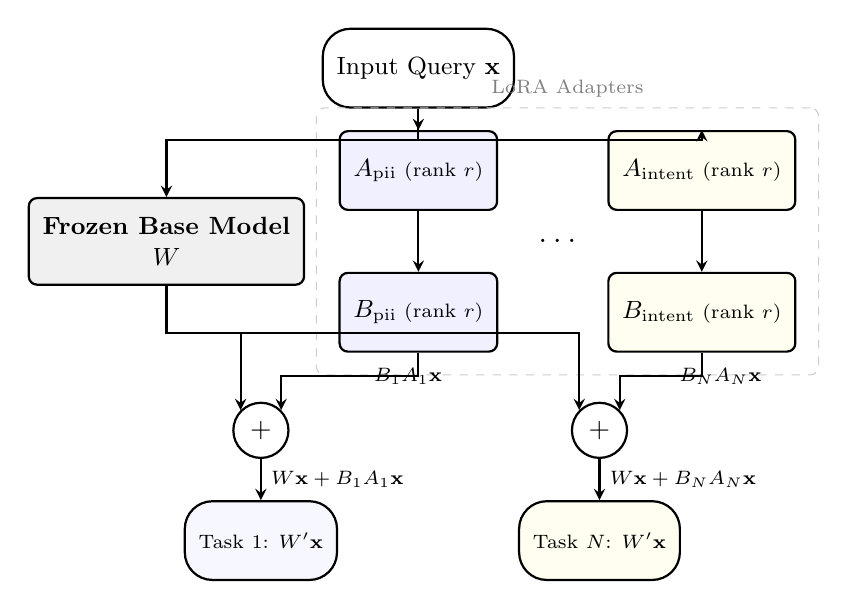
\begin{tikzpicture}[
      box/.style={rectangle, draw, thick, rounded corners=3pt,
                  minimum height=1cm, align=center, inner sep=5pt, font=\small},
      adapter/.style={box, minimum width=1.8cm},
      sum/.style={circle, draw, thick, inner sep=0pt, minimum size=0.7cm,
                  font=\normalsize},
      outbox/.style={box, rounded corners=10pt},
      arr/.style={->, >=stealth, thick},
      lbl/.style={font=\scriptsize, midway},
    ]

    % Input
    \node[outbox] (input) at (3.2, 5.2) {Input Query $\mathbf{x}$};

    % Frozen base model
    \node[box, fill=black!6, minimum width=2.6cm, thick,
          minimum height=1.1cm] (base) at (0, 3)
      {\textbf{Frozen Base Model}\\$W$};

    % Adapter group 1 (PII) -- left
    \node[adapter, fill=blue!6] (a1) at (3.2, 3.9) {$A_{\text{pii}}$\;\scriptsize(rank $r$)};
    \node[adapter, fill=blue!6] (b1) at (3.2, 2.1) {$B_{\text{pii}}$\;\scriptsize(rank $r$)};

    % Dots
    \node[font=\large] at (5.0, 3) {\dots};

    % Adapter group N (intent) -- right
    \node[adapter, fill=yellow!6] (an) at (6.8, 3.9) {$A_{\text{intent}}$\;\scriptsize(rank $r$)};
    \node[adapter, fill=yellow!6] (bn) at (6.8, 2.1) {$B_{\text{intent}}$\;\scriptsize(rank $r$)};

    % Adapters bounding box
    \node[rectangle, draw, dashed, gray!40, rounded corners=3pt,
          fit=(a1)(bn)(an), inner sep=8pt, label={[font=\scriptsize,gray]above:LoRA Adapters}] {};

    % Sum nodes
    \node[sum] (s1) at (1.2, 0.6) {$+$};
    \node[sum] (sn) at (5.5, 0.6) {$+$};

    % Outputs
    \node[outbox, fill=blue!3] (o1) at (1.2, -0.8) {\scriptsize Task 1: $W'\mathbf{x}$};
    \node[outbox, fill=yellow!6] (on) at (5.5, -0.8) {\scriptsize Task $N$: $W'\mathbf{x}$};

    % Arrows: input to base and adapters
    \draw[arr] (input.south) -- ++(0,-0.4) -| (base.north);
    \draw[arr] (input) -- (a1);
    \draw[arr] (input.south) -- ++(0,-0.4) -| (an.north);

    % Arrows: A to B within adapters
    \draw[arr] (a1) -- (b1);
    \draw[arr] (an) -- (bn);

    % Arrows: base to sum nodes
    \draw[arr] (base.south) -- ++(0,-0.6) -| (s1.north west);
    \draw[arr] (base.south) -- ++(0,-0.6) -| (sn.north west);

    % Arrows: adapters to sum nodes
    \draw[arr] (b1.south) -- ++(0,-0.3) -|
      node[lbl, right, pos=0.2] {\scriptsize $B_1 A_1 \mathbf{x}$} (s1.north east);
    \draw[arr] (bn.south) -- ++(0,-0.3) -|
      node[lbl, right, pos=0.2] {\scriptsize $B_N A_N \mathbf{x}$} (sn.north east);

    % Arrows: sum to output
    \draw[arr] (s1) -- node[lbl, right] {\scriptsize $W\mathbf{x} + B_1 A_1 \mathbf{x}$} (o1);
    \draw[arr] (sn) -- node[lbl, right] {\scriptsize $W\mathbf{x} + B_N A_N \mathbf{x}$} (on);

    \end{tikzpicture}
    \caption{LoRA-based MoM inference architecture. The input query~$\mathbf{x}$ is processed by a single frozen base model~($W$). Each task-specific LoRA adapter pair ($A_i$, $B_i$) computes a low-rank perturbation $B_i A_i \mathbf{x}$. The base output and adapter perturbation are summed to produce task-specific classifications, enabling multi-task support with minimal memory overhead.}
    \label{fig:lora_arch}
\end{figure}

Note that LoRA does \emph{not} eliminate the per-task forward pass---each adapter requires a full inference through the modified model.
The primary benefit is \textbf{memory efficiency}: deploying six classifiers requires the memory footprint of approximately one model rather than six, and all adapters can be updated independently without reloading the base model.

\subsection{MoM Model Family}

We train a family of purpose-built models (MoM: Mixture-of-Models) optimized for routing classification tasks:

\begin{table}[h]
\centering
\caption{MoM model family.
All models share a common base (ModernBERT~\cite{warner2024modernbert} or mmBERT-32K) and are distributed as LoRA adapters.}
\label{tab:mom_family}
\begin{tabular}{lll}
\toprule
\textbf{Model} & \textbf{Task} & \textbf{Training Data} \\
\midrule
\texttt{mom-domain}         & Domain classification     & MMLU categories \\
\texttt{mom-pii}            & PII token classification  & Presidio-annotated corpora \\
\texttt{mom-jailbreak}      & Prompt injection detection & Adversarial prompt datasets \\
\texttt{mom-sentinel}       & Fact-check gating         & Factual vs.\ creative queries \\
\texttt{mom-detector}       & Hallucination detection   & Annotated LLM outputs \\
\texttt{mom-explainer}      & NLI explanation           & NLI benchmarks \\
\texttt{mom-feedback}       & User feedback analysis    & Conversation annotations \\
\texttt{mom-modality}       & Modality classification   & DiffusionDB + text corpora \\
\texttt{mom-embedding}      & Semantic embeddings       & Contrastive pre-training \\
\texttt{mom-toolcall}       & Tool selection            & Function-calling datasets \\
\texttt{mom-intent} & User intent classification & Customer support dialogues \\
\bottomrule
\end{tabular}
\end{table}

The key benefit of distributing these as LoRA adapters rather than independent models is \textbf{operational simplicity}: a single base model binary serves all ten tasks, adapters can be hot-swapped without reloading the base, and new tasks can be added by training a new adapter without retraining or redistributing the base model.

\subsection{Training Methodology}

All LoRA adapters are trained using PEFT~\cite{mangrulkar2022peft} with the following protocol:
\begin{itemize}[leftmargin=*]
  \item \textbf{Base model}: ModernBERT or mmBERT-32K (for long-context tasks).
  \item \textbf{Adapter configuration}: Rank $r \in \{16, 32, 64\}$, applied to query and value projection matrices.
  \item \textbf{Training}: Task-specific datasets with standard cross-entropy loss.
  \item \textbf{Export}: Both LoRA-only (separate adapter files for hot-swapping) and merged (single model file for simplified deployment) formats.
\end{itemize}

The modality classifier, for instance, is trained on a balanced mixture of DiffusionDB (image generation prompts), OASST2, Alpaca, and Dolly (text generation), achieving three-class classification (autoregressive, diffusion, both) with $\sim$0.02\% trainable parameters relative to the base model.


% --- Model Selection Algorithms ---
% sections/model_selection.tex

\section{Semantic Model Selection}
\label{sec:model_selection}

The core routing innovation is \emph{semantic model selection}: once the decision engine matches a routing decision $d^*$, the system analyzes the request's semantic content---its embedding, domain, complexity, and interaction history---to select the most cost-effective model from the decision's candidate set.
Unlike static routing or single-criterion difficulty classifiers, semantic selection operates over the full signal context produced by the signal engine, enabling cost-quality optimization that respects per-decision privacy and safety constraints.

We integrate thirteen algorithms within a unified interface, enabling systematic comparison and hybrid combinations across deployment scenarios.

\subsection{Problem Setting}

Given query embedding $\mathbf{e}_q \in \mathbb{R}^d$, domain category $z \in \{1, \ldots, C\}$, candidate models $\mathcal{M}_{d^*} = \{m_1, \ldots, m_K\}$ with associated costs $\{c_1, \ldots, c_K\}$, and quality estimators, the semantic selection problem is:
\begin{equation}
  m^* = \arg\max_{m_k \in \mathcal{M}_{d^*}} \; \text{Quality}(\mathbf{e}_q, z, m_k; \Theta) - \lambda \cdot \text{Cost}(m_k)
\end{equation}
where $\lambda \geq 0$ is a cost-sensitivity parameter and $\Theta$ represents algorithm-specific parameters.
The per-decision candidate set $\mathcal{M}_{d^*}$ is critical: privacy-constrained decisions restrict candidates to compliant models, while cost-optimized decisions include a broader pool with aggressive cost weighting.
We categorize algorithms into families based on their selection mechanism (\Cref{fig:selection_taxonomy}).

\begin{figure}[t]
\centering
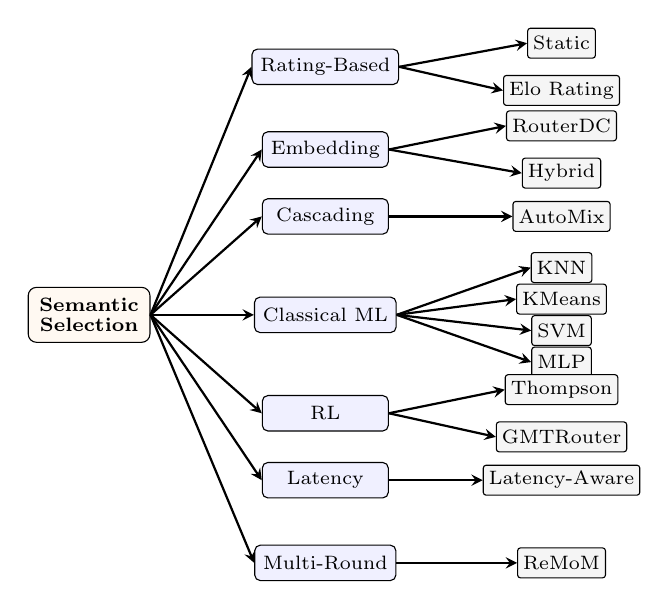
\begin{tikzpicture}[
    node distance=0.2cm,
    fam/.style={rectangle, draw, rounded corners=2pt, fill=blue!6,
                minimum height=0.45cm, minimum width=1.6cm,
                align=left, font=\scriptsize, inner sep=3pt},
    alg/.style={rectangle, draw, rounded corners=1pt, fill=black!4,
                minimum height=0.38cm, align=left,
                font=\scriptsize, inner sep=2pt},
    root/.style={rectangle, draw, rounded corners=3pt, fill=orange!5,
                 minimum height=0.5cm, align=center,
                 font=\scriptsize\bfseries, inner sep=4pt},
    edge from parent/.style={draw, thick, ->, >=stealth},
    level 1/.style={sibling distance=1.05cm, level distance=2.6cm},
  ]
  % Root
  \node[root] (rt) at (0, 0) {Semantic\\[-1pt]Selection};

  % Families (y positions)
  \node[fam] (f1) at (3.0, 3.15) {Rating-Based};
  \node[fam] (f2) at (3.0, 2.1) {Embedding};
  \node[fam] (f3) at (3.0, 1.25) {Cascading};
  \node[fam] (f4) at (3.0, 0.0) {Classical ML};
  \node[fam] (f5) at (3.0, -1.25) {RL};
  \node[fam] (f6) at (3.0, -2.1) {Latency};
  \node[fam] (f7) at (3.0, -3.15) {Multi-Round};

  % Algorithms
  \node[alg] (a1) at (6.0, 3.45) {Static};
  \node[alg] (a2) at (6.0, 2.85) {Elo Rating};
  \node[alg] (a3) at (6.0, 2.4) {RouterDC};
  \node[alg] (a4) at (6.0, 1.8) {Hybrid};
  \node[alg] (a5) at (6.0, 1.25) {AutoMix};
  \node[alg] (a6) at (6.0, 0.6) {KNN};
  \node[alg] (a7) at (6.0, 0.2) {KMeans};
  \node[alg] (a8) at (6.0, -0.2) {SVM};
  \node[alg] (a9) at (6.0, -0.6) {MLP};
  \node[alg] (a10) at (6.0, -0.95) {Thompson};
  \node[alg] (a11) at (6.0, -1.55) {GMTRouter};
  \node[alg] (a12) at (6.0, -2.1) {Latency-Aware};
  \node[alg] (a13) at (6.0, -3.15) {ReMoM};

  % Root → Families
  \foreach \f in {f1,f2,f3,f4,f5,f6,f7}
    \draw[thick, ->, >=stealth] (rt.east) -- (\f.west);

  % Families → Algorithms
  \draw[thick, ->, >=stealth] (f1.east) -- (a1.west);
  \draw[thick, ->, >=stealth] (f1.east) -- (a2.west);
  \draw[thick, ->, >=stealth] (f2.east) -- (a3.west);
  \draw[thick, ->, >=stealth] (f2.east) -- (a4.west);
  \draw[thick, ->, >=stealth] (f3.east) -- (a5.west);
  \draw[thick, ->, >=stealth] (f4.east) -- (a6.west);
  \draw[thick, ->, >=stealth] (f4.east) -- (a7.west);
  \draw[thick, ->, >=stealth] (f4.east) -- (a8.west);
  \draw[thick, ->, >=stealth] (f4.east) -- (a9.west);
  \draw[thick, ->, >=stealth] (f5.east) -- (a10.west);
  \draw[thick, ->, >=stealth] (f5.east) -- (a11.west);
  \draw[thick, ->, >=stealth] (f6.east) -- (a12.west);
  \draw[thick, ->, >=stealth] (f7.east) -- (a13.west);
\end{tikzpicture}
\caption{Taxonomy of thirteen semantic model selection algorithms organized by selection mechanism.  Families span from lightweight rating-based methods (Static, Elo) to learned approaches (RouterDC, Classical ML, RL), adaptive cascading (AutoMix), real-time latency tracking, and multi-round synthesis (ReMoM).}
\label{fig:selection_taxonomy}
\end{figure}

\subsection{Rating-Based Selection}

\noindent\textbf{Static.}
Each model carries a pre-configured quality score $s_k$; selection is $m^* = \arg\max_k s_k$.
Serves as a deterministic baseline.

\noindent\textbf{Elo Rating} (adapted from RouteLLM~\cite{ong2024routellm}).
Models maintain Elo ratings $R_k$ updated from pairwise user preference feedback.
Selection probability follows the Bradley-Terry model:
\begin{equation}
  P(m_i \succ m_j) = \frac{1}{1 + 10^{(R_j - R_i)/400}}
\end{equation}
Models are sampled proportional to their expected win rate against the candidate pool.
Ratings are updated online as user feedback arrives.

\subsection{Embedding-Based Selection}

\noindent\textbf{RouterDC}~\cite{chen2024routerdc}.
Dual contrastive learning trains query and model encoders to produce embeddings in a shared space.
Selection maximizes cosine similarity:
\begin{equation}
  m^* = \arg\max_{m_k \in \mathcal{M}_{d^*}} \cos(\mathbf{e}_q, \mathbf{e}_{m_k})
\end{equation}
The contrastive training objective encourages queries to be close to their best-performing model's embedding and distant from poorly-performing models.

\noindent\textbf{Hybrid}~\cite{hu2024routerbench}.
Combines Elo ratings, embedding similarity, and cost in a weighted score:
\begin{equation}
  \text{score}(m_k) = \alpha \cdot \tilde{R}_k + \beta \cdot \cos(\mathbf{e}_q, \mathbf{e}_{m_k}) + \gamma \cdot (1 - \tilde{c}_k)
\end{equation}
where $\tilde{R}_k$ and $\tilde{c}_k$ are normalized ratings and costs, and $\alpha + \beta + \gamma = 1$ are configurable weights.

\subsection{Cascading Selection}

\noindent\textbf{AutoMix}~\cite{aggarwal2023automix}.
Formulated as a Partially Observable Markov Decision Process (POMDP).
Models are ordered by capability $m_1 \prec m_2 \prec \cdots \prec m_K$.
The cascade:
\begin{enumerate}
  \item Generate response $a_k$ with current model $m_k$ (starting from $k=1$, the cheapest).
  \item Self-verify: estimate response quality $\hat{q}_k$ using $m_k$ itself.
  \item If $\hat{q}_k \geq \tau_k$, accept $a_k$; otherwise, escalate to $m_{k+1}$.
\end{enumerate}
The expected cost is:
\begin{equation}
  \mathbb{E}[C] = \sum_{k=1}^{K} C_k \cdot \prod_{j=1}^{k-1}(1 - P(\hat{q}_j \geq \tau_j))
\end{equation}
where $P(\hat{q}_j \geq \tau_j)$ is the probability that model $m_j$ passes self-verification.
This naturally trades off cost against quality.

\subsection{Classical ML Selection}

These methods train on routing records $\{(\mathbf{e}_q^{(i)}, z^{(i)}, m^{*(i)}, q^{(i)})\}$ where $q^{(i)}$ is a quality score.
Feature vectors combine embeddings and domain information:
\begin{equation}
  \mathbf{f} = [\mathbf{e}_q \in \mathbb{R}^d; \; \text{onehot}(z) \in \{0,1\}^C]
\end{equation}

\noindent\textbf{KNN.}
$k$-nearest neighbor search with Ball Tree indexing.
Quality-weighted majority voting:
\begin{equation}
  m^* = \arg\max_m \sum_{i \in \text{kNN}(\mathbf{f})} \mathbf{1}[m^{*(i)} = m] \cdot q^{(i)}
\end{equation}

\noindent\textbf{KMeans.}
Assigns queries to pre-computed clusters; selects the best model for the assigned cluster based on a combined quality-latency score:
\begin{equation}
  m^* = \arg\max_m \bigl(\alpha \cdot \text{quality}(m, z_\text{cluster}) - (1-\alpha) \cdot \text{latency}(m)\bigr)
\end{equation}

\noindent\textbf{SVM.}
Multi-class SVM with RBF or linear kernel, trained to classify feature vectors directly into model selections.

\noindent\textbf{MLP.}
A feed-forward neural network (two hidden layers with ReLU activation) mapping $\mathbf{f}$ to a softmax distribution over candidate models:
\begin{equation}
  P(m_k \mid \mathbf{f}) = \text{softmax}\bigl(W_2 \cdot \text{ReLU}(W_1 \mathbf{f} + b_1) + b_2\bigr)_k
\end{equation}
The MLP is implemented in the GPU-accelerated Candle runtime for low-latency inference.

\subsection{Reinforcement Learning Selection}

\noindent\textbf{Thompson Sampling}~\cite{thompson1933likelihood}.
Each model maintains a Beta prior:
\begin{equation}
  \theta_k \sim \text{Beta}(\alpha_k, \beta_k)
\end{equation}
Selection samples from each posterior and picks the maximum: $m^* = \arg\max_k \theta_k$.
Parameters $(\alpha_k, \beta_k)$ are updated from user preference feedback, naturally balancing exploration and exploitation.

\noindent\textbf{GMTRouter}~\cite{xie2025gmtrouter}.
Models multi-turn user-query-model interactions as a heterogeneous graph.
Graph neural network message passing captures complex interaction patterns:
\begin{equation}
  \mathbf{h}_v^{(l+1)} = \text{AGG}\bigl(\{\mathbf{h}_u^{(l)} \mid u \in \mathcal{N}(v)\}\bigr)
\end{equation}
where nodes represent users, queries, and models, and edges encode historical routing outcomes.

\subsection{Latency-Aware Selection}

\noindent\textbf{Latency-Aware.}
Selects the model with the best observed latency using percentile-based Time-per-Output-Token (TPOT) and Time-to-First-Token (TTFT) statistics collected at runtime.
For each candidate model $m_k$, the selector computes a normalized latency score:
\begin{equation}
  s_k = \frac{1}{|P|} \sum_{p \in P} \frac{\text{perc}_p(m_k)}{\min_{j}\, \text{perc}_p(m_j)}
\end{equation}
where $P \subseteq \{\text{TPOT}, \text{TTFT}\}$ is the set of configured performance metrics and $\text{perc}_p(m_k)$ is the observed percentile value for model $m_k$ on metric $p$.
Selection minimizes this score: $m^* = \arg\min_k s_k$.
This enables adaptive routing that responds to real-time backend performance degradation without requiring explicit latency thresholds as signal conditions.

\subsection{Multi-Round Reasoning (ReMoM)}

The ReMoM (Reasoning for Mixture of Models) strategy extends single-shot selection to multi-round parallel reasoning with LLM-driven synthesis.
Inspired by PaCoRe~\cite{pacore2025} but generalized to heterogeneous model pools, ReMoM executes a \emph{breadth schedule} of decreasing parallelism across rounds, where each subsequent round synthesizes the outputs of the previous round via prompted LLM calls (\Cref{fig:remom_flow}).

\begin{figure}[t]
\centering
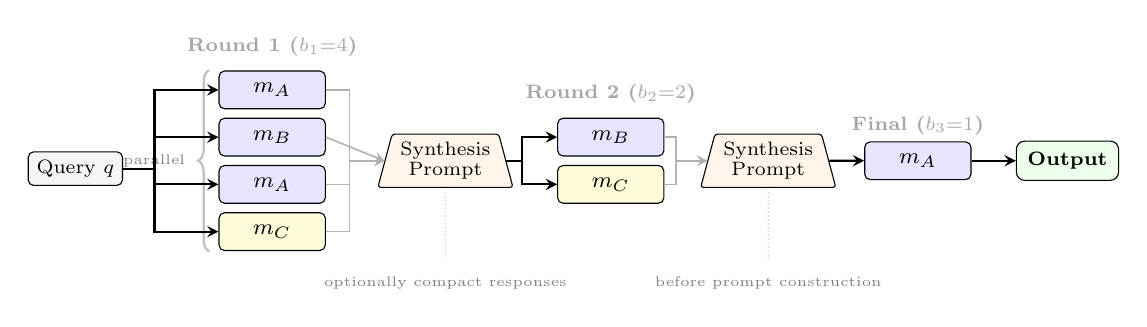
\begin{tikzpicture}[
    node distance=0.3cm,
    call/.style={rectangle, draw, rounded corners=2pt,
                 minimum height=0.48cm, minimum width=1.35cm,
                 align=center, font=\scriptsize, inner sep=2pt},
    synth/.style={trapezium, draw, trapezium angle=75, rounded corners=1pt,
                  fill=orange!8, minimum height=0.5cm,
                  align=center, font=\scriptsize, inner sep=3pt},
    query/.style={rectangle, draw, rounded corners=2pt, fill=black!4,
                  font=\scriptsize, inner sep=3pt, align=center},
    outbox/.style={rectangle, draw, rounded corners=3pt, fill=green!8,
                   font=\scriptsize\bfseries, inner sep=4pt, align=center},
    roundlbl/.style={font=\scriptsize\bfseries, text=gray!70},
    arr/.style={->, >=stealth, thick},
    arrs/.style={->, >=stealth, semithick, gray!60},
  ]

  % === Query ===
  \node[query] (q) at (0, 0) {Query $q$};

  % === Round 1: b_1 = 4 ===
  \node[roundlbl] at (2.5, 1.55) {Round 1 ($b_1{=}4$)};
  \node[call, fill=blue!10]   (r1c1) at (2.5, 1.0)  {\footnotesize $m_A$};
  \node[call, fill=blue!10]   (r1c2) at (2.5, 0.4)  {\footnotesize $m_B$};
  \node[call, fill=blue!10]   (r1c3) at (2.5, -0.2) {\footnotesize $m_A$};
  \node[call, fill=yellow!15] (r1c4) at (2.5, -0.8) {\footnotesize $m_C$};

  % Parallel bracket
  \draw[decorate, decoration={brace, amplitude=4pt, mirror}, thick, gray!50]
    (1.7, 1.25) -- (1.7, -1.05) node[midway, left=5pt, font=\tiny, text=gray] {parallel};

  % Query → Round 1
  \draw[arr] (q.east) -- ++(0.4,0) |- (r1c1.west);
  \draw[arr] (q.east) -- ++(0.4,0) |- (r1c2.west);
  \draw[arr] (q.east) -- ++(0.4,0) |- (r1c3.west);
  \draw[arr] (q.east) -- ++(0.4,0) |- (r1c4.west);

  % === Synthesis 1 ===
  \node[synth] (s1) at (4.7, 0.1) {Synthesis\\[-1pt]Prompt};

  % Round 1 → Synthesis 1
  \draw[arrs] (r1c1.east) -- ++(0.3,0) |- (s1.west);
  \draw[arrs] (r1c2.east) -- (s1.west);
  \draw[arrs] (r1c3.east) -- ++(0.3,0) |- (s1.west);
  \draw[arrs] (r1c4.east) -- ++(0.3,0) |- (s1.west);

  % === Round 2: b_2 = 2 ===
  \node[roundlbl] at (6.8, 0.95) {Round 2 ($b_2{=}2$)};
  \node[call, fill=blue!10]   (r2c1) at (6.8, 0.4)  {\footnotesize $m_B$};
  \node[call, fill=yellow!15] (r2c2) at (6.8, -0.2) {\footnotesize $m_C$};

  % Synthesis 1 → Round 2
  \draw[arr] (s1.east) -- ++(0.2,0) |- (r2c1.west);
  \draw[arr] (s1.east) -- ++(0.2,0) |- (r2c2.west);

  % === Synthesis 2 ===
  \node[synth] (s2) at (8.8, 0.1) {Synthesis\\[-1pt]Prompt};

  % Round 2 → Synthesis 2
  \draw[arrs] (r2c1.east) -- ++(0.15,0) |- (s2.west);
  \draw[arrs] (r2c2.east) -- ++(0.15,0) |- (s2.west);

  % === Round 3: b_3 = 1 (final) ===
  \node[roundlbl] at (10.7, 0.55) {Final ($b_3{=}1$)};
  \node[call, fill=blue!10] (r3c1) at (10.7, 0.1) {\footnotesize $m_A$};

  % Synthesis 2 → Round 3
  \draw[arr] (s2.east) -- (r3c1.west);

  % === Output ===
  \node[outbox] (out) at (12.6, 0.1) {Output};
  \draw[arr] (r3c1.east) -- (out.west);

  % === Compaction annotation ===
  \node[font=\tiny, text=gray, anchor=north] at (4.7, -1.25)
    {optionally compact responses};
  \draw[densely dotted, gray!40] (4.7, -1.15) -- (s1.south);
  \draw[densely dotted, gray!40] (8.8, -1.15) -- (s2.south);
  \node[font=\tiny, text=gray, anchor=north] at (8.8, -1.25)
    {before prompt construction};

\end{tikzpicture}
\caption{ReMoM execution flow with breadth schedule $\mathbf{b} = [4, 2]$.
Round~1 distributes 4~parallel calls across models ($m_A$, $m_B$, $m_C$); responses are (optionally compacted and) assembled into a synthesis prompt.
Round~2 sends 2~parallel synthesis calls.
A final round ($b_3 = 1$, auto-appended) produces the single output.
Each synthesis prompt includes the original query and all previous-round responses as numbered references, delegating quality judgment to the synthesizing LLM.}
\label{fig:remom_flow}
\end{figure}

\noindent\textbf{Breadth schedule.}
The operator specifies a breadth schedule $\mathbf{b} = [b_1, b_2, \ldots, b_R]$ defining the number of parallel model calls per round.
A final synthesis round with $b_{R+1} = 1$ is automatically appended, yielding a total of $R+1$ rounds.
For example, $\mathbf{b} = [32, 4]$ produces three rounds: 32 parallel calls, then 4 parallel calls each synthesizing the 32 responses, then a single final call synthesizing the 4 responses.

\noindent\textbf{Model distribution.}
At each round, $b_r$ calls are distributed among the candidate models $\mathcal{M}_{d^*}$ according to one of three strategies:
(1)~\emph{equal}: calls are distributed evenly across all candidates with round-robin remainder allocation;
(2)~\emph{weighted}: calls are distributed proportionally to model weights (currently equivalent to equal distribution);
(3)~\emph{first\_only}: all $b_r$ calls target a single model with different random seeds, providing PaCoRe-compatible single-model diversity.
Calls within each round execute concurrently with configurable concurrency limits.

\noindent\textbf{LLM-driven synthesis.}
After collecting responses from round $r$, the system constructs a synthesis prompt for round $r+1$ using a configurable Go \texttt{text/template}.
The default template presents the original query alongside all previous-round responses as numbered references, instructing the next-round model(s) to \emph{``analyze these references and provide your own comprehensive solution.''}
When reasoning content is available (e.g., from models supporting extended thinking), the template additionally includes each reference's chain-of-thought reasoning.
This approach delegates quality judgment entirely to the synthesizing LLM rather than relying on explicit scoring or weighted aggregation.

\noindent\textbf{Response compaction.}
To manage prompt length across rounds, responses can be compacted before inclusion in synthesis prompts.
Two strategies are supported: \emph{full} (no compaction, the default) and \emph{last\_n\_tokens} (retaining only the final $N$ tokens, estimated at $\sim$4 characters per token).
This is particularly important for high-breadth schedules where concatenating all responses would exceed context limits.

\noindent\textbf{Execution flow.}
The complete algorithm proceeds as:
\begin{enumerate}
  \item \textbf{Schedule construction}: Append $[1]$ to the user-specified breadth schedule $\mathbf{b}$.
  \item \textbf{Round~1 (parallel generation)}: Distribute $b_1$ calls across candidate models; execute concurrently with temperature $T$ (default 1.0) for response diversity.
  \item \textbf{Rounds~$2 \ldots R{+}1$ (synthesis)}: For each subsequent round, build a synthesis prompt from the previous round's (optionally compacted) responses, distribute $b_r$ calls, and execute concurrently.
  \item \textbf{Final output}: Return the single response from the final round ($b_{R+1} = 1$).
\end{enumerate}

ReMoM is particularly effective when model capabilities are uncertain or when the task benefits from diverse perspectives (e.g., complex reasoning, multi-faceted analysis).
The breadth schedule provides fine-grained control over the cost--quality tradeoff: higher initial breadth increases diversity at the cost of additional LLM calls, while the funneling structure ensures convergence to a single synthesized answer.

\subsection{Unified Selection Interface}

All thirteen algorithms implement a common interface:
\begin{equation}
  \text{Select}: (\mathbf{e}_q, z, \mathcal{M}, \Theta) \to (m^*, c)
\end{equation}
returning the selected model and a confidence score.
This uniformity enables:
(1)~per-decision algorithm selection---different routing decisions can use different selection algorithms, allowing cost-optimized decisions to use cascading (AutoMix) while quality-sensitive decisions use embedding-based (RouterDC) selection;
(2)~A/B testing across algorithms on live traffic;
(3)~ensemble methods that combine multiple selectors.

\subsection{Cost-Aware Selection in Multi-Provider Settings}

In multi-endpoint deployments where the same logical model may be served by different providers at different price points, the selection algorithms operate in conjunction with the endpoint router (\Cref{subsec:multi_endpoint}).
The selection algorithm chooses the best \emph{model} based on semantic analysis, and the endpoint router resolves it to the most cost-effective \emph{provider endpoint}.
This two-stage process separates quality optimization (which model is best for this query?) from cost optimization (which provider endpoint offers the best price for this model?), enabling fine-grained cost management across heterogeneous multi-cloud deployments.


% --- ML Inference Bindings ---
% sections/ml_inference.tex

\section{Multi-Runtime ML Inference}
\label{sec:ml_inference}

The routing system requires low-latency ML inference for signal extraction, classification, and embedding computation---all on the critical path of every request.
We describe the multi-runtime architecture that addresses the tension between inference speed, hardware flexibility, and model diversity.

\subsection{Design Constraints}

Three constraints shape the inference architecture:
\begin{enumerate}
  \item \textbf{Latency}: Signal extraction must complete within the tail latency budget of the routing system (target: $<$100\,ms for all signals combined).
  \item \textbf{Hardware heterogeneity}: Deployments range from GPU-equipped data centers to CPU-only edge nodes.
  \item \textbf{Model diversity}: Different tasks require different model architectures (sequence classification, token classification, NLI, embeddings, MLP).
\end{enumerate}

\subsection{Three-Runtime Architecture}

We implement three inference runtimes, each optimized for different hardware and task profiles, all exposed to the routing layer via C FFI:

\begin{table}[h]
\centering
\caption{Inference runtime characteristics}
\label{tab:runtimes}
\begin{tabular}{llll}
\toprule
\textbf{Runtime} & \textbf{Target Hardware} & \textbf{Tasks} & \textbf{Framework} \\
\midrule
Candle   & GPU (CUDA), CPU & Classification, LoRA, MLP & HF Candle~\cite{candleml2024} \\
Linfa    & CPU only        & KNN, KMeans, SVM         & Linfa~\cite{linfa2024} \\
ONNX RT  & CPU, GPU        & Embeddings               & ONNX Runtime~\cite{onnxruntime2024} \\
\bottomrule
\end{tabular}
\end{table}

All runtimes are compiled as Rust shared libraries and linked to the Go routing process via CGo.
This eliminates Python runtime overhead, GIL contention, and inter-process communication latency that would arise from serving models in separate Python processes.

\subsection{Candle Runtime: GPU-Accelerated Classification}

The Candle runtime handles all transformer-based classification tasks, including LoRA adapter loading and inference (\Cref{sec:lora_mom}).

\textbf{Supported architectures.}
BERT~\cite{devlin2019bert}, ModernBERT~\cite{warner2024modernbert} (with Flash Attention and GeGLU), mmBERT-32K (YaRN RoPE for 32K context), DeBERTa v3 (NLI), and feed-forward MLPs (model selection).

\textbf{Optimization features.}
Flash Attention 2 kernels reduce attention memory from $O(n^2)$ to $O(n)$ and improve throughput.
Optional Intel MKL integration for CPU deployments.
LoRA adapter hot-loading enables runtime model updates without restart.

\subsection{Linfa Runtime: CPU ML Inference}

Classical ML model selection algorithms (KNN, KMeans, SVM) are served by the Linfa runtime.
These algorithms operate on pre-computed feature vectors and do not require GPU acceleration, making Linfa's lightweight CPU implementation ideal.

\textbf{Training-inference split.}
Models are trained in Python (scikit-learn, custom implementations) and serialized to JSON.
The Rust runtime loads serialized models at startup and performs inference-only computation.
This decouples the training environment (Python, GPU-optional) from the inference environment (Rust, CPU-only), enabling simpler deployment.

\subsection{ONNX Runtime: Efficient Embeddings}

Embedding computation is served by ONNX Runtime, optimized for the mmBERT-Embed-32K model with 2D Matryoshka representation learning~\cite{kusupati2022matryoshka}.

\textbf{2D Matryoshka trade-offs.}
The architecture supports two-dimensional quality-latency trade-offs:
\begin{itemize}[leftmargin=*]
  \item \textbf{Layer early-exit}: Extract embeddings from intermediate layers (6, 11, 16, or 22 out of 22), achieving $\sim$3--4$\times$ speedup at layer 6 with modest quality degradation.
  \item \textbf{Dimension truncation}: Reduce embedding dimension from 768 to 64, 128, 256, or 512, reducing memory and computation for similarity search.
\end{itemize}

For the $\sim$150M parameter embedding model, CPU inference with 2D Matryoshka (layer 11, dimension 256) achieves latency comparable to GPU inference on the full model, making GPU optional for embedding computation.

\subsection{Runtime Selection Strategy}

The routing system selects runtimes based on deployment configuration:
\begin{itemize}[leftmargin=*]
  \item \textbf{GPU available}: Candle (classification + LoRA) + ONNX (embeddings) + Linfa (ML selection).
  \item \textbf{CPU only}: Candle with MKL (classification) + ONNX with early-exit (embeddings) + Linfa (ML selection).
  \item \textbf{Minimal}: ONNX (embeddings) + Linfa (ML selection), with classification delegated to external vLLM-served models.
\end{itemize}

\paragraph{Contributors.}
Huamin Chen, yehudit1987, Xunzhuo, abdallahsamabd, Yue Zhu, OneZero-Y, shown, Yossi Ovadia, cryo, Xunzhuo, aias00, Wilson Wu, Tien Nguyen, Srinivas A, Qiping Pan, Nengxing Shen, Liav Weiss, GuanMu, ERIK.


% --- ExtProc Pipeline ---
% sections/extproc_pipeline.tex

\section{Request Processing Pipeline}
\label{sec:extproc}

We implement the routing system as an Envoy External Processor (ExtProc)~\cite{envoyextproc2024}, enabling transparent interception of LLM API traffic without client-side modifications.
This section describes the pipeline architecture, multi-provider routing, the Responses API integration, and the pluggable authorization factory.

\subsection{Transparent Interception via ExtProc}

The Envoy ExtProc protocol~\cite{envoyextproc2024} establishes a bidirectional gRPC stream between the proxy and the routing service for each HTTP request.
Envoy invokes the processor at four phases---request headers, request body, response headers, response body---and the processor responds with mutations (header modifications, body rewrites) or immediate responses (short-circuiting the backend).

This architecture provides two key advantages:
(1)~\emph{transparency}: clients send standard OpenAI-compatible API requests to the proxy endpoint with no awareness of the routing layer; and
(2)~\emph{composability}: the router coexists with other Envoy filters (rate limiting, authentication, load balancing) in the standard filter chain.

\subsection{Request Body Pipeline}

The request body phase implements the core routing logic as a sequential pipeline:

\begin{equation}
  r \xrightarrow{\text{parse}} r' \xrightarrow{\text{signals}} S(r') \xrightarrow{\text{decide}} d^* \xrightarrow{\Pi_\text{pre}} \xrightarrow{\text{select}} m^* \xrightarrow{\text{route}} e^*
\end{equation}

The stages execute in strict order:
(1)~API translation (Responses API $\to$ Chat Completions if applicable, see \Cref{subsec:responses_api});
(2)~request parsing and provider detection;
(3)~signal extraction and decision evaluation (\Cref{sec:signal_engine,sec:decision_engine});
(4)~jailbreak detection (\Cref{sec:safety});
(5)~PII detection (\Cref{sec:safety});
(6)~semantic cache lookup (\Cref{sec:plugins})---cache hits terminate the pipeline with an immediate response;
(7)~RAG context injection (\Cref{sec:memory_rag});
(8)~modality routing (text vs.\ diffusion);
(9)~memory retrieval (\Cref{sec:memory_rag});
(10)~model selection (\Cref{sec:model_selection}), system prompt injection, and header mutation;
(11)~multi-endpoint resolution and provider-specific auth injection (\Cref{subsec:multi_endpoint,subsec:authz_factory}).

\subsection{Multi-Endpoint and Multi-Provider Routing}
\label{subsec:multi_endpoint}

Production deployments often span multiple model backends across different providers and geographic regions.
The system supports \emph{multi-endpoint routing} as a first-class concept:

\begin{definition}[Endpoint Topology]
An endpoint topology $\mathcal{E} = \{(e_i, w_i, p_i, \alpha_i)\}_{i=1}^{L}$ defines $L$ endpoints, each with a weight $w_i \in (0, 1]$ (normalized: $\sum_i w_i = 1$), a provider type $p_i \in \mathcal{P}$, and an auth profile $\alpha_i$.
\end{definition}

Once semantic model selection identifies a target model $m^*$, the endpoint router resolves $m^*$ to a concrete endpoint $e^*$ from the set of endpoints serving that model.
Weighted random selection with sticky session affinity distributes load proportionally.
Failover cascades to the next-weighted endpoint on backend errors.

Each endpoint may use a different provider (e.g., the same logical model ``gpt-4o'' served by both OpenAI and Azure OpenAI).
The system performs \emph{provider-specific protocol translation} transparently:

\begin{itemize}[leftmargin=*]
  \item \textbf{OpenAI / Azure OpenAI}: Native Chat Completions and Responses API formats.
  \item \textbf{Anthropic}: Translation between OpenAI message schema and Anthropic Messages API (system prompt handling, tool use mapping).
  \item \textbf{Bedrock / Vertex AI}: Cloud-provider-specific request wrapping, authentication (SigV4 for AWS, OAuth for GCP), and response unwrapping.
  \item \textbf{Gemini}: Conversion between OpenAI function-calling schema and Gemini tool declarations.
  \item \textbf{vLLM / Local}: Direct OpenAI-compatible passthrough to self-hosted vLLM instances.
\end{itemize}

This abstraction allows routing decisions to reference models by capability (``best coding model'') rather than by provider-specific endpoint, and allows the same decision configuration to operate across different deployment topologies.

\subsection{OpenAI Responses API Support}
\label{subsec:responses_api}

The system provides full support for the OpenAI Responses API, which extends Chat Completions with stateful multi-turn conversation management.

The Responses API introduces \texttt{previous\_response\_id} chaining: each response carries a unique identifier, and subsequent requests can reference it to maintain conversation context without the client retransmitting the full message history.
The routing system handles this by:

\begin{enumerate}[leftmargin=*]
  \item \textbf{Inbound translation}: Responses API requests (with \texttt{input} field and \texttt{previous\_response\_id}) are normalized to Chat Completions format for signal extraction and decision evaluation, which operate on the unified internal representation.
  \item \textbf{State management}: Conversation history is stored in the persistent memory layer (\Cref{sec:memory_rag}), keyed by response ID, enabling context retrieval across turns.
  \item \textbf{Outbound translation}: Chat Completions responses from backends are wrapped in Responses API format (with \texttt{id}, \texttt{output} array, \texttt{usage} breakdown) before returning to the client.
  \item \textbf{Routing consistency}: The decision engine can optionally pin conversation turns to the same model to avoid mid-conversation quality shifts.
\end{enumerate}

This translation layer is transparent to both the signal engine and the downstream model backends, enabling all routing, safety, and caching features to operate identically on Responses API and Chat Completions traffic.

\subsection{Authorization Factory}
\label{subsec:authz_factory}

Multi-provider deployments require diverse authentication mechanisms.
The system implements a \emph{pluggable authorization factory} that abstracts auth concerns from routing logic:

\begin{definition}[Auth Provider]
An auth provider $\alpha: (\text{Request}, \text{Endpoint}) \to \text{Headers}'$ is a function that enriches outbound request headers with provider-appropriate credentials.
\end{definition}

The factory supports multiple auth provider types:

\begin{itemize}[leftmargin=*]
  \item \textbf{API Key}: Static bearer tokens or API keys, optionally per-endpoint, with header name customization (e.g., \texttt{Authorization}, \texttt{x-api-key}, \texttt{api-key}).
  \item \textbf{OAuth2 / OIDC}: Token acquisition with automatic refresh, supporting client credentials and authorization code flows.
  \item \textbf{Cloud IAM}: AWS SigV4 signing for Bedrock, Google service account tokens for Vertex AI, Azure AD tokens for Azure OpenAI.
  \item \textbf{Passthrough}: Forwarding the client's original credentials to the backend, used for deployments where the client authenticates directly.
  \item \textbf{Custom}: User-defined auth plugins registered at startup, enabling integration with enterprise identity providers (LDAP, SAML, custom JWT issuers).
\end{itemize}

The auth factory is invoked \emph{after} decision evaluation and model selection, injecting provider-specific credentials into the outbound request headers.
This separation ensures that routing decisions are auth-agnostic: the decision engine selects models based on capability and cost, and the auth layer handles the mechanics of reaching each provider's endpoint.

The \texttt{authz} signal type in the signal engine (\Cref{sec:signal_engine}) is complementary but distinct: it performs \emph{inbound} authorization (verifying that the requesting user or API key has permission to access specific models or decisions), while the auth factory handles \emph{outbound} authentication (proving the router's identity to backend providers).

\subsection{Response Body Pipeline}

The response path performs:
(1)~token usage extraction for cost accounting;
(2)~format translation (provider-specific $\to$ OpenAI format);
(3)~streaming metrics computation (TTFT, TPOT);
(4)~hallucination detection via HaluGate (\Cref{sec:halugate});
(5)~semantic cache writes for cache misses;
(6)~Responses API translation (Chat Completions $\to$ Responses API format, if applicable).

\subsection{Concurrency Model}

Each gRPC stream (one per HTTP request) runs in an independent goroutine, processing its four phases sequentially.
Within a request, signal extraction launches parallel coroutines for independent classifiers.
Shared state (classifier models, cache backends, configuration, auth token caches) is read concurrently by all active streams, with synchronization limited to cache writes, auth token refreshes, and metric updates.

\paragraph{Contributors.}
Xunzhuo, Huamin Chen, Jintao Zhang, Xunzhuo, asaadbalum, OneZero-Y, Noa Limoy, Liav Weiss, yehudit1987, shown, Yossi Ovadia, Alex Wang, cryo, abdallahsamabd, Senan Zedan, R3hankhan, Fang Han, samzong, aeft, Srinivas A, Sanjeev Rampal, Qiping Pan, Nengxing Shen, Jared, Avishek Goswami, Avinash Changrani, AkisAya.


% --- Memory + RAG ---
% sections/memory_rag.tex

\section{Memory and Retrieval-Augmented Generation}
\label{sec:memory_rag}

Production routing systems must support multi-turn conversations with persistent context and knowledge-augmented responses.
We describe the memory and RAG subsystems that operate as plugins within the routing pipeline.

\subsection{Persistent Memory}

The memory system maintains user-scoped knowledge across conversation sessions, enabling personalized routing and context-aware responses.
\Cref{fig:memory_lifecycle} illustrates the full memory lifecycle.

\textbf{Memory extraction.}
An LLM-based extractor analyzes conversation turns to identify user-specific facts, classified into three types:
\emph{semantic} (factual knowledge: preferences, background),
\emph{procedural} (workflows, how-to knowledge), and
\emph{episodic} (specific events and interactions).

\textbf{Deduplication.}
Before storage, extracted facts undergo similarity-based deduplication against existing memories, preventing redundant entries that would degrade retrieval precision.

\textbf{Retrieval gating.}
Not every query benefits from memory retrieval.
A lightweight heuristic determines whether memory search is warranted by filtering out general fact-check queries, tool-augmented requests, and simple greetings, avoiding unnecessary embedding lookups and reducing latency for queries where personal context is irrelevant.

\textbf{Retrieval.}
At query time, relevant memories are retrieved via embedding similarity search over the user's memory store, formatted as context, and injected into the system message.
An optional query-rewriting step reformulates the user's query for improved retrieval recall.

\textbf{Retention scoring and pruning.}
Memory stores grow unbounded without lifecycle management.
We adopt an exponential decay model inspired by the Ebbinghaus forgetting curve~\cite{zhong2023memorybank}:
\begin{equation}
  R = e^{-t/S}, \quad S = S_0 + n_{\text{access}}
\end{equation}
where $t$ is the time in days since last retrieval, $S_0$ is the initial strength (default 30 days), and $n_{\text{access}}$ is the cumulative access count.
Each retrieval reinforces the memory by incrementing $n_{\text{access}}$, slowing future decay.
Memories falling below a retention threshold $R < \delta$ become pruning candidates.
An optional per-user capacity limit evicts the lowest-scoring entries when the store exceeds a configurable maximum.

\begin{figure}[H]
\centering
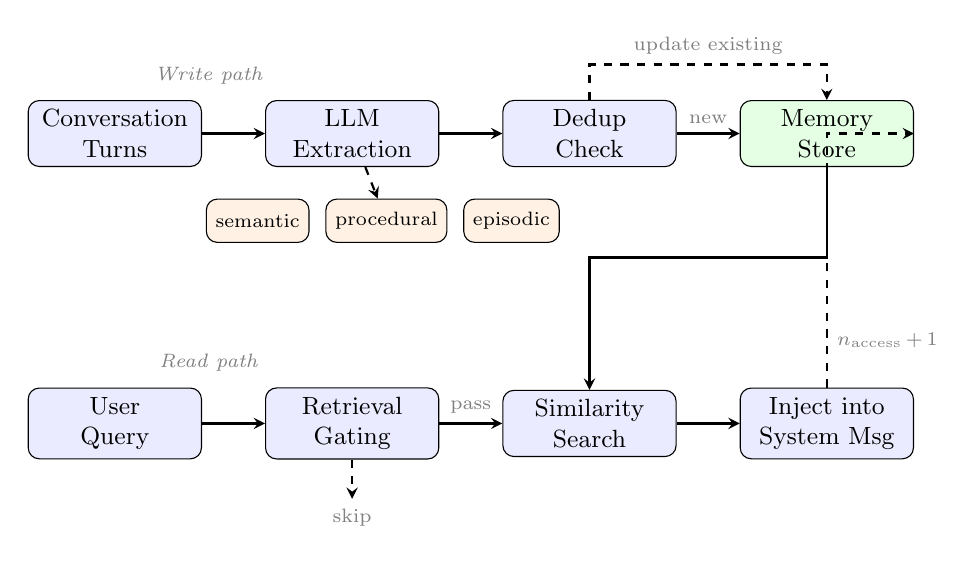
\begin{tikzpicture}[
    node distance=0.6cm and 0.8cm,
    box/.style={draw, rounded corners, fill=blue!8, minimum width=2.2cm,
                minimum height=0.8cm, align=center, font=\small},
    storebox/.style={draw, rounded corners, fill=green!10, minimum width=2.2cm,
                minimum height=0.8cm, align=center, font=\small},
    typebox/.style={draw, rounded corners, fill=orange!10,
                minimum height=0.55cm, align=center, font=\scriptsize},
    arr/.style={->, >=stealth, thick},
    darr/.style={->, >=stealth, thick, dashed},
    lbl/.style={font=\scriptsize, text=gray}
]

% --- Write path (top row) ---
\node[box] (conv) {Conversation\\Turns};
\node[box, right=of conv] (extract) {LLM\\Extraction};
\node[box, right=of extract] (dedup) {Dedup\\Check};
\node[storebox, right=of dedup] (store) {Memory\\Store};

\draw[arr] (conv) -- (extract);
\draw[arr] (extract) -- (dedup);
\draw[arr] (dedup) -- node[above, lbl] {new} (store);

% Memory types below extraction
\node[typebox, below=0.4cm of extract, xshift=-1.2cm] (sem) {semantic};
\node[typebox, right=0.2cm of sem] (proc) {procedural};
\node[typebox, right=0.2cm of proc] (epis) {episodic};
\draw[darr] (extract) -- (proc);

% Dedup "update existing" loops back above store
\draw[darr] (dedup.north) -- ++(0,0.45) -| node[above, lbl, pos=0.25] {update existing} (store.north);

% --- Read path (bottom row) ---
\node[box, below=2.8cm of conv] (query) {User\\Query};
\node[box, right=of query] (gate) {Retrieval\\Gating};
\node[box, right=of gate] (retrieve) {Similarity\\Search};
\node[box, right=of retrieve] (inject) {Inject into\\System Msg};

\draw[arr] (query) -- (gate);
\draw[arr] (gate) -- node[above, lbl] {pass} (retrieve);
\draw[arr] (retrieve) -- (inject);

% Store feeds into retrieval
\draw[arr] (store.south) -- ++(0,-1.15) -| (retrieve.north);

% Skip arrow from gate
\draw[darr] (gate.south) -- ++(0,-0.5) node[below, lbl] {skip};

% Retrieval reinforces memory (feedback arrow on the right)
\draw[darr] (inject.north) -- ++(0,0.6) node[right, lbl] {$n_{\text{access}}$\,+\,1} |- (store.east);

% --- Path labels ---
\node[lbl, above=0.08cm of conv, xshift=1.2cm] {\textit{Write path}};
\node[lbl, above=0.08cm of query, xshift=1.2cm] {\textit{Read path}};

\end{tikzpicture}
\caption{Memory lifecycle. The write path extracts facts from conversations, deduplicates against existing entries, and stores new memories. The read path gates retrieval, searches by embedding similarity, and injects context. Each retrieval increments $n_{\text{access}}$, reinforcing the memory's retention score.}
\label{fig:memory_lifecycle}
\end{figure}

\subsection{Retrieval-Augmented Generation}

The RAG plugin retrieves relevant documents from vector stores and injects them as context before model invocation.

\textbf{Indexing pipeline.}
Documents are chunked (configurable size and overlap), embedded using the shared embedding model (\Cref{sec:ml_inference}), and indexed in a vector store.

\textbf{Retrieval.}
For each request, the query embedding is computed and the top-$k$ most similar chunks are retrieved via approximate nearest neighbor search.
Retrieved chunks are formatted and injected into the prompt as additional context.

\textbf{Backend abstraction.}
Vector stores are accessed through a common interface supporting in-memory (development), Milvus~\cite{wang2021milvus} (production), and file-based (persistent, no external dependencies) backends.

\subsection{Stateful Conversations (Response API)}

The system supports the OpenAI Responses API for stateful multi-turn conversations:

\textbf{Conversation chaining.}
Each response is stored with a unique ID.
Subsequent requests reference \texttt{previous\_response\_id} to reconstruct the full conversation history.
A bidirectional translator converts between the Response API format and Chat Completions format for backend model invocation.

\textbf{Routing continuity.}
Stored responses include routing metadata (decision, model selection, signal results), enabling consistent routing across conversation turns and providing context for feedback-driven model selection.

\textbf{State backends.}
Conversation state is persisted via in-memory (development), Redis (distributed), or Milvus (semantic retrieval) backends.

\subsection{Integration with Signal-Decision Architecture}

Both memory and RAG operate as per-decision plugins.
Different decisions can activate different RAG configurations (different vector stores, different $k$ values, different chunk strategies) or disable retrieval entirely.
This enables, for example, a ``research assistant'' decision that activates RAG with a technical knowledge base while a ``casual chat'' decision disables retrieval.


% --- Observability ---
% sections/observability.tex

\section{Observability}
\label{sec:observability}

Intelligent routing introduces a new observability surface: beyond standard model serving metrics, operators must monitor signal extraction quality, decision matching patterns, plugin effectiveness, and model selection outcomes.

\subsection{Metrics Taxonomy}

We instrument four metric categories using Prometheus~\cite{prometheus2024}:

\noindent\textbf{Model performance.}
Per-model request counts, token usage, estimated cost, completion latency, Time-to-First-Token (TTFT), and Time-per-Output-Token (TPOT).
These metrics enable real-time cost monitoring and performance regression detection across the model fleet.

\noindent\textbf{Routing behavior.}
Routing modification counts (original model vs.\ selected model), reason codes (which signal types triggered which decisions), and routing latency (overhead of the routing pipeline itself).
These metrics answer the question: \emph{how is the router changing traffic patterns?}

\noindent\textbf{Signal and decision quality.}
Per-signal-type extraction counts and match rates, per-decision match frequencies and confidence distributions, and per-plugin execution counts and outcomes.
These metrics enable calibration: if a signal type rarely matches, its threshold may need adjustment; if a decision matches too broadly, its conditions may be under-specified.

\noindent\textbf{Safety and cache effectiveness.}
PII violation rates by entity type, jailbreak detection rates, hallucination detection latency, cache hit rates, and cache operation latency.
These metrics quantify the value delivered by the plugin chain.

\subsection{Distributed Tracing}

We implement OpenTelemetry~\cite{opentelemetry2024} tracing with a hierarchical span model:
\begin{itemize}[leftmargin=*]
  \item \textbf{Root span}: Covers the full request lifecycle from receipt to response.
  \item \textbf{Signal spans}: Individual spans for each signal type evaluation, capturing latency and results.
  \item \textbf{Decision span}: Decision evaluation with the matched decision and confidence.
  \item \textbf{Plugin spans}: Per-plugin execution with type-specific attributes (cache hit/miss, PII types detected, hallucination spans found).
  \item \textbf{Upstream span}: Backend model invocation, with W3C Trace Context propagation enabling end-to-end tracing through vLLM~\cite{kwon2023vllm} and other inference frameworks.
\end{itemize}

This span hierarchy enables operators to diagnose routing latency (``which signal is slow?''), understand routing decisions (``why was this query routed to model X?''), and correlate routing behavior with model serving performance.


% --- Deployment ---
% sections/deployment.tex

\section{Deployment}
\label{sec:deployment}

We describe the deployment architecture that enables the routing system to operate from single-node development to production Kubernetes clusters.

\subsection{Deployment Modes}

\textbf{Local development.}
A single command (\texttt{pip install vllm-sr \&\& vllm-sr serve}) bootstraps the complete stack: router, Envoy proxy, and dashboard.
This lowers the barrier to experimentation with routing configurations.

\textbf{Kubernetes: Standalone mode.}
Envoy runs as a sidecar container alongside the router in the same pod.
The ExtProc filter connects via localhost gRPC.
Deployed via Helm charts with configurable replicas, resource limits, cache backends, and autoscaling.

\textbf{Kubernetes: Gateway mode.}
The router runs as an independent service behind an existing Istio or Envoy Gateway deployment, referenced via the gateway's ExtProc configuration.
This mode shares the gateway infrastructure across multiple services.

\subsection{Kubernetes Operator}

A custom operator manages the lifecycle of routing deployments through a \texttt{SemanticRouter} Custom Resource Definition (CRD).
The reconciliation loop manages: service accounts, configuration (ConfigMap or CRD-sourced), persistent storage, gateway/route resources, Envoy configuration, deployments, services, and horizontal pod autoscalers.

\textbf{Backend discovery.}
The operator discovers model backends via three mechanisms:
KServe InferenceService resources (for managed model serving),
label-based Llama Stack discovery, and
direct Kubernetes Service references.

\subsection{Dashboard}

A web console (React frontend, Go backend) provides:
configuration editing with live validation,
topology visualization of routing flows,
an interactive playground for testing routing decisions,
embedded Grafana/Prometheus/Jaeger dashboards for monitoring and tracing, and
an evaluation framework for benchmarking routing quality.


% --- Evaluation ---
% sections/evaluation.tex

\section{Evaluation}
\label{sec:evaluation}

We evaluate the routing system across three dimensions: signal extraction efficiency, LoRA multi-task scaling, and end-to-end routing correctness.

\subsection{Signal Extraction Latency}

\Cref{tab:signal_latency} reports median and p99 latencies for each signal type on an NVIDIA A100 GPU with ModernBERT base model.

\begin{table}[h]
\centering
\caption{Signal extraction latency by type}
\label{tab:signal_latency}
\begin{tabular}{lrrl}
\toprule
\textbf{Signal Type} & \textbf{Median} & \textbf{p99} & \textbf{Requires ML} \\
\midrule
Keyword      & $< 0.1$\,ms & $< 0.5$\,ms  & No \\
Context      & $< 0.1$\,ms & $< 0.5$\,ms  & No \\
Language     & $< 0.5$\,ms & $< 1$\,ms    & No \\
Authorization & $< 0.1$\,ms & $< 0.5$\,ms & No \\
\midrule
Embedding    & $15$\,ms    & $45$\,ms     & Yes \\
Domain       & $60$\,ms    & $120$\,ms    & Yes \\
Fact-check   & $55$\,ms    & $110$\,ms    & Yes \\
Modality     & $50$\,ms    & $100$\,ms    & Yes \\
Feedback     & $55$\,ms    & $115$\,ms    & Yes \\
Complexity   & $50$\,ms    & $105$\,ms    & Yes \\
Preference   & $55$\,ms    & $110$\,ms    & Yes \\
\bottomrule
\end{tabular}
\end{table}

Heuristic signals complete in sub-millisecond time, while ML signals range from 15--120\,ms.
With parallel evaluation, the wall-clock time is dominated by the slowest active signal ($\sim$120\,ms for domain classification) rather than the sum.

\subsection{LoRA Memory Efficiency}

\Cref{tab:lora_memory} shows the memory advantage of serving classifiers via LoRA adapters versus independent fine-tuned models.

\begin{table}[h]
\centering
\caption{Model memory: independent fine-tuned models vs.\ LoRA adapters (ModernBERT base, 150M params)}
\label{tab:lora_memory}
\begin{tabular}{lrr}
\toprule
\textbf{Tasks ($n$)} & \textbf{Independent (MB)} & \textbf{LoRA (MB)} \\
\midrule
1 & 573   & 573 \\
3 & 1{,}719 & 574 \\
6 & 3{,}438 & 575 \\
\bottomrule
\end{tabular}
\end{table}

At $n = 6$, the LoRA architecture requires $\sim$6$\times$ less model memory (one base model + six $\sim$0.2\,MB adapters vs.\ six full model copies).
Each task still requires its own forward pass; latency reduction comes from \emph{parallel execution} of classifiers rather than from LoRA itself (\Cref{sec:lora_mom}).

\subsection{Decision Engine Overhead}

Decision evaluation adds negligible latency:
$< 0.1$\,ms for 10 decisions with 3 conditions each;
$< 0.5$\,ms for 100 decisions with 5 conditions each.
This confirms that the $O(M \cdot L_\text{max})$ complexity is dominated by signal extraction.

\subsection{Composable Orchestration Across Deployment Scenarios}

A key claim of this work is that the same architecture serves diverse deployment scenarios through configuration.
\Cref{tab:deployment_scenarios} demonstrates how different signal-decision-plugin compositions address different requirements:

\begin{table}[h]
\centering
\caption{Composable signal orchestration across deployment scenarios. Each scenario activates a different subset of the eleven signal types, selection algorithms, and plugin chains---using the same system binary and architecture.}
\label{tab:deployment_scenarios}
\begin{tabular}{p{2.5cm}p{3cm}p{2.5cm}p{3.5cm}}
\toprule
\textbf{Scenario} & \textbf{Active Signals} & \textbf{Selection} & \textbf{Key Plugins} \\
\midrule
Privacy-regulated (healthcare) & authz, domain, language & Static (compliant models only) & Strict PII redaction, no caching, audit logging \\
Cost-optimized (developer tool) & complexity, embedding, keyword & AutoMix cascade & Aggressive semantic cache, header mutation for LoRA adapter \\
Multi-cloud enterprise & domain, modality, authz & Latency-aware & Multi-endpoint failover, provider auth factory, system prompt injection \\
Multi-turn assistant & embedding, feedback, preference & Elo with session pin & Responses API state, memory retrieval, RAG injection \\
\bottomrule
\end{tabular}
\end{table}

\subsection{End-to-End Routing Correctness}

The end-to-end test framework validates routing behavior across eight scenario profiles:

\begin{table}[h]
\centering
\caption{End-to-end test profiles}
\label{tab:e2e_profiles}
\begin{tabular}{lp{8cm}}
\toprule
\textbf{Profile} & \textbf{Validated Behavior} \\
\midrule
Multi-endpoint      & Multi-provider routing with weighted distribution and failover across heterogeneous backends \\
Multi-provider auth & Provider-specific auth injection (API key, OAuth2, cloud IAM) via authorization factory \\
AuthZ-RBAC          & Role-based model access (admin/premium/free tiers) with authz signal \\
ML model selection  & KNN, KMeans, SVM, MLP selection accuracy on held-out queries \\
Keyword routing     & Keyword signal matching with AND/OR/NOR combinators \\
Embedding routing   & Embedding similarity thresholds and confidence-based decision selection \\
RAG + Responses API & Context retrieval, injection, and stateful multi-turn via Responses API \\
Routing strategies  & Static, Elo, RouterDC, AutoMix, Hybrid algorithm comparison \\
\bottomrule
\end{tabular}
\end{table}

Each profile validates correct model selection, safety enforcement (jailbreak blocked, PII detected), cache behavior (hits after similar queries), multi-provider routing (correct endpoint resolution and auth injection), and header propagation.

\subsection{Semantic Cache Effectiveness}

At a similarity threshold $\theta = 0.92$:
exact-match queries achieve 100\% hit rate with $< 5$\,ms lookup latency;
paraphrased queries achieve 60--80\% hit rate depending on paraphrase distance.
Cache hits eliminate backend model invocation entirely, reducing per-request cost to embedding computation only.

\subsection{Unified MoM Evaluation Framework}

To ensure the robustness of the Mixture of Models (MoM) collection, we developed a unified evaluation pipeline capable of assessing both merged models and LoRA adapters across diverse tasks (Text and Token Classification).

The framework, illustrated in \Cref{fig:eval_pipeline}, addresses the heterogeneity of the 10+ active models by standardizing the evaluation flow.Key architectural features include:

\begin{itemize}
    \item \textbf{Dynamic Data Alignment:} Specialized data loaders normalize inputs from diverse sources, including MMLU-Pro for intent classification and synthetic Presidio data for PII detection, while automatically filtering samples by language (e.g., distinguishing between \texttt{es}, \texttt{fr}, \texttt{zh}) to validate cross-lingual performance.
    \item \textbf{LoRA vs. Merged Comparison:} The pipeline supports toggleable evaluation between full fine-tuned checkpoints and LoRA adapters loaded onto the \texttt{ModernBERT-base} backbone, ensuring that the memory efficiency gains described in \Cref{tab:lora_memory} do not come at the cost of predictive quality.
    \item \textbf{Robust Parallel Inference:} To handle large-scale benchmarks, the system utilizes \texttt{ProcessPoolExecutor} for parallel model evaluation with built-in OOM (Out-Of-Memory) recovery and exponential backoff strategies for network reliability.
\end{itemize}

We report comprehensive metrics including accuracy, weighted F1-score, and per-class precision/recall, alongside p50/p99 latency profiling to verify that model quality meets production standards before deployment.

\begin{figure}[h]
    \centering
    \includegraphics[width=\linewidth]{figures/evaluation_flow.svg}
    \caption{The Unified MoM Evaluation Pipeline. The system parallelizes evaluation across the model registry, handling dynamic dataset loading (Presidio, MMLU-Pro), language filtering, and comparative metrics generation for both Merged and LoRA model variants.}
    \label{fig:eval_pipeline}
\end{figure}

\paragraph{Contributors.}
Senan Zedan, Xunzhuo, yehudit1987, abdallahsamabd, Noa Limoy, Yossi Ovadia, Liav Weiss, Huamin Chen, samzong, Jintao Zhang, asaadbalum, Xunzhuo, Srinivas A, Marina Koushnir, Chever John, Chaojun Zhang, Avishek Goswami, Zohaib Hassnain.




% --- Related Work ---
% sections/related_work.tex

\section{Related Work}
\label{sec:related_work}

\subsection{LLM Routing and Model Selection}

\textbf{Binary routing.}
RouteLLM~\cite{ong2024routellm} pioneered preference-data-driven routing between a strong and weak model, training BERT, MLP, and causal LLM classifiers to estimate query difficulty.
Our work extends this to multi-model, multi-signal routing with per-decision plugin chains.

\textbf{Contrastive selection.}
RouterDC~\cite{chen2024routerdc} learns shared query-model embeddings via dual contrastive learning.
We integrate RouterDC as one of thirteen selection algorithms and extend it with signal-conditioned features (domain category, complexity).

\textbf{Cascading.}
AutoMix~\cite{aggarwal2023automix} formulates model cascading as a POMDP with self-verification.
We integrate AutoMix within our plugin-aware framework, where safety checks and caching can prevent unnecessary escalation.

\textbf{Benchmarking.}
RouterBench~\cite{hu2024routerbench} proposed a benchmark for multi-LLM routing with hybrid scoring.
Our Hybrid selector builds on this approach.

\textbf{RL-based routing.}
Router-R1~\cite{zhang2025routerr1} applies reinforcement learning with Thompson sampling for multi-round routing.
GMTRouter~\cite{xie2025gmtrouter} uses graph-based learning for personalized multi-turn interactions.
We integrate both within the unified selection interface and extend them with the ReMoM multi-round reasoning strategy.

A key distinction of our work is that prior approaches address model selection in isolation, while we embed selection within a composable signal orchestration framework that also handles signal extraction, safety enforcement, caching, context augmentation, and multi-provider routing---enabling the same selection algorithms to serve fundamentally different deployment scenarios through configuration.

\subsection{Multi-Provider and Multi-Endpoint Routing}

Commercial LLM gateway products (OpenRouter, AWS Bedrock, Azure AI Studio) provide multi-provider access but lack the composable signal-driven routing that enables differentiated policies per routing decision.
API management platforms (Kong, Apigee) offer gateway functionality but are not designed for semantic analysis of LLM requests.
Our system uniquely combines semantic model selection with multi-provider protocol abstraction, a pluggable authorization factory, and full OpenAI Responses API support for stateful conversations within the same composable framework.

\subsection{Mixture-of-Experts vs.\ Mixture-of-Models}

Sparse Mixture-of-Experts (MoE)~\cite{shazeer2017moe,jiang2024mixtral} routes \emph{tokens} to specialized sub-networks \emph{within} a single model architecture.
Our system operates at the \emph{request level}, routing entire requests across \emph{different model deployments}---a Mixture-of-Models (MoM) approach.
The two paradigms are complementary: our router can route to MoE models as backends.

\subsection{LLM Safety}

Prompt injection defenses~\cite{jain2023promptguard,inan2023llamaguard} detect adversarial inputs via fine-tuned classifiers.
PII detection systems~\cite{lison2021anonymisation} identify sensitive information using rule-based and ML approaches.
Our safety subsystem integrates both within the routing pipeline with per-decision thresholds and policies, using LoRA adapters for memory-efficient multi-task classification.

\subsection{Hallucination Detection}

SelfCheckGPT~\cite{manakul2023selfcheckgpt} detects hallucinations via multi-sample consistency.
FActScore~\cite{min2023factscore} evaluates factual precision at the atomic fact level.
HaluGate differs in three respects:
(1)~a gating Sentinel that skips verification for non-factual queries;
(2)~token-level span identification rather than sentence-level scoring;
(3)~NLI-based explanation distinguishing contradiction from neutral unsupported content.

\subsection{Semantic Caching and RAG}

Semantic caching for LLMs~\cite{lewis2020rag} uses embedding similarity for query matching.
Our cache extends this with per-decision policies, multiple backends, and integration with the safety pipeline (cache lookups occur \emph{after} safety checks but \emph{before} model invocation).
RAG integration~\cite{lewis2020rag,wang2021milvus} augments responses with retrieved context; our contribution is embedding RAG as a per-decision plugin within the routing framework.


% --- Conclusion ---
% sections/conclusion.tex

\section{Conclusion}
\label{sec:conclusion}

We have presented \sysname{}, a signal-driven decision routing system for Mixture-of-Modality model deployments.
The central contribution is \textbf{composable signal orchestration}: the three-layer architecture---signal extraction, Boolean decision evaluation, per-decision plugin chains---enables diverse deployment scenarios to be expressed as different configurations over the same framework, without code changes.

Privacy-regulated deployments activate authz and PII signals with strict filtering plugins; cost-optimized deployments enable cascading selection with aggressive semantic caching; multi-cloud enterprises configure weighted multi-endpoint routing with provider-specific auth injection.
All use the same signal-decision-plugin machinery, composed differently.

Within this framework, \textbf{semantic model selection} analyzes each request's content through thirteen algorithms---spanning rating-based, contrastive, cascading, classical ML, reinforcement learning, and latency-aware families---to find the most cost-effective model while respecting per-decision privacy and safety constraints.
The integration of full \textbf{OpenAI Responses API support} enables stateful multi-turn routing with conversation-consistent model assignment; \textbf{multi-endpoint and multi-provider routing} abstracts over heterogeneous backends (vLLM, OpenAI, Anthropic, Azure, Bedrock, Gemini, Vertex AI) with transparent protocol translation; and the \textbf{pluggable authorization factory} supports diverse auth mechanisms across providers without coupling auth logic to routing decisions.

Additional technical contributions include:
(1)~the LoRA-based multi-task classification architecture that serves $n$ classifiers from a single base model, reducing aggregate model memory by $\sim$$n\times$;
(2)~HaluGate's gated three-stage hallucination detection pipeline that reduces average detection cost by $\sim$50\% through sentinel-based filtering; and
(3)~Rust-native ML inference bindings (Candle, Linfa, ONNX Runtime) that achieve sub-10\,ms signal extraction latency.

The system has been validated in production with over 600 merged contributions from 50+ engineers and is deployed as an Envoy ExtProc with Kubernetes operator support.

\subsection{Future Directions}

Several research directions emerge from this work:

\textbf{Learned decision policies.}
Replacing hand-crafted Boolean rules with learned routing policies (e.g., neural routing networks trained on production traffic) could improve routing quality while maintaining interpretability through attention-based explanation.

\textbf{Adaptive cost optimization.}
Online learning approaches that continuously adapt model and provider selection based on real-time cost signals, latency measurements, and user feedback---extending the current offline-trained ML selectors to fully adaptive cost-quality optimization.

\textbf{Cross-provider consistency.}
Techniques for ensuring consistent behavior when routing the same conversation across different providers, addressing differences in instruction following, safety behavior, and output formatting.

\textbf{Multi-turn safety.}
Extending safety enforcement from single-turn to multi-turn conversations, detecting adversarial patterns that span multiple interaction rounds.

\textbf{Federated signal orchestration.}
Extending composable signal orchestration to federated deployments where signals from multiple routing instances are aggregated for global optimization.

\textbf{Multi-protocol adapter abstraction.}
The current system is tightly coupled to Envoy's External Processor protocol. A multi-protocol adapter architecture would abstract the routing engine from protocol-specific code, enabling support for HTTP REST, native gRPC, Nginx/OpenResty, and custom protocols through thin translation layers.
This would also enable abstraction of backend proxying (currently Envoy-specific), external authorization mechanisms, and traffic management policies, making the routing engine truly protocol-agnostic and deployable in serverless, edge, and non-Envoy environments.

\subsection*{Acknowledgments}

We gratefully acknowledge contributions who contributed to the project.
We thank the Hugging Face Candle team for collaboration on the Candle inference runtime, and the Envoy community for the ExtProc filter.
AMD has sponsored the project with resources and infrastructure as well as the vLLM project for the development of the project.
AI-assisted tools were used during the writing and proofreading of this paper.
The project is open-source at \url{https://github.com/vllm-project/semantic-router}.


% --- Bibliography ---
\bibliographystyle{iclr2026_conference}
\bibliography{references}

\end{document}
